\documentclass[10pt,twocolumn,letterpaper]{article}
\usepackage[T1]{fontenc}
\usepackage{iccv}
\usepackage{times}

\usepackage[font={footnotesize}]{caption}
\usepackage[linesnumbered, ruled]{algorithm2e}
\usepackage[percent]{overpic}
\usepackage{amsmath}
\usepackage{amssymb}
\usepackage{booktabs}
\usepackage{color}
\usepackage{comment}
\usepackage{contour}
\usepackage{dsfont}
\usepackage{floatrow}
\usepackage{graphicx}
\usepackage{layouts}
\usepackage{listings}
\usepackage{multirow}
\usepackage{subcaption}
\usepackage{tabularx}
\usepackage{tcolorbox}
\usepackage{transparent}
\usepackage{url}
\usepackage{verbatim}
\usepackage{xspace}

\usepackage[pagebackref=true,breaklinks=true,letterpaper=true,colorlinks,bookmarks=false]{hyperref}
%\usepackage[capitalise]{cleveref}
\usepackage{cleveref}

\iccvfinalcopy
\def\iccvPaperID{3193}
\ificcvfinal\pagestyle{empty}\fi

\newfloatcommand{capbtabbox}{table}[][\FBwidth]

\newcommand{\mytodo}[1]{{\noindent\textcolor{red}{TODO: #1}}}
\newcommand{\todo}[1]{\mytodo{#1}}
\newcommand{\bbf}{\mathbf{f}}
\newcommand{\bx}{\mathbf{x}}
\newcommand{\by}{\mathbf{y}}
\newcommand{\bz}{\mathbf{z}}
\newcommand{\bw}{\mathbf{w}}
\newcommand{\be}{\mathbf{e}}
\newcommand{\bv}{\mathbf{v}}
\newcommand{\methodname}{Invariant Information Clustering\xspace}
\newcommand{\methodnameshort}{IIC\xspace}
\newcommand{\bdash}{\mathbf{'}}
\newcommand{\bc}{\mathbf{c}}
\newcommand{\defeq}{\overset{\Delta}{=}}
\newcommand{\cmt}[1]{\ignorespaces}

\newcommand{\matP}{\mathbf{P}}  %\boldsymbol{P}

% Default fixed font does not support bold face
\DeclareFixedFont{\ttb}{T1}{txtt}{bx}{n}{6.5} % for bold
\DeclareFixedFont{\ttm}{T1}{txtt}{m}{n}{6.5}  % for normal

% Suppress annoying badness warnings (disable for final version).
\hfuzz=10000pt
\vfuzz=10000pt
\hbadness=2000
\vbadness=\maxdimen

% No space paragraph.
\makeatletter
\renewcommand{\paragraph}{%
  \@startsection{paragraph}{4}%
  %{\z@}{3.25ex \@plus 1ex \@minus .2ex}{-1em}%
  {\z@}{0.5em}{-1em}%
  {\normalfont\normalsize\bfseries}%
}
\makeatother

\DeclareMathOperator*{\argmax}{argmax}
\DeclareMathOperator*{\argmin}{argmin}

% General parameters, for ALL pages:
\renewcommand{\topfraction}{0.9}    % max fraction of floats at top
\renewcommand{\bottomfraction}{0.8} % max fraction of floats at bottom

% Parameters for TEXT pages (not float pages):
\setcounter{topnumber}{2}
\setcounter{bottomnumber}{2}
\setcounter{totalnumber}{4} % 2 may work better
\setcounter{dbltopnumber}{2} % for 2-column pages
\renewcommand{\dbltopfraction}{0.9} % fit big float above 2-col. text
\renewcommand{\textfraction}{0.07} % allow minimal text w. figs

% Parameters for FLOAT pages (not text pages):
\renewcommand{\floatpagefraction}{0.7} % require fuller float pages

% N.B.: floatpagefraction MUST be less than topfraction !!
\renewcommand{\dblfloatpagefraction}{0.7} % require fuller float pages

% Separation between text and figure etc
\setlength{\textfloatsep}{5.0pt plus 2.0pt minus 4.0pt}
\setlength{\floatsep}{5.0pt plus 2.0pt minus 2.0pt}
\setlength{\intextsep}{5.0pt plus 2.0pt minus 2.0pt}
\setlength{\dbltextfloatsep}{5.0pt plus 2.0pt minus 2.0pt}
\setlength{\dblfloatsep}{5.0pt plus 2.0pt minus 2.0pt}

\floatsetup[table]{capposition=bottom,captionskip=0.2em}
\floatsetup[figure]{capposition=bottom,captionskip=0.2em}

\title{\methodname for \\ Unsupervised Image Classification and Segmentation}
\author{Xu Ji\\
University of Oxford\\
{\tt\small xuji@robots.ox.ac.uk}
\and
Jo\~ao F. Henriques\\
University of Oxford\\
{\tt\small joao@robots.ox.ac.uk}
\and
Andrea Vedaldi\\
University of Oxford\\
{\tt\small vedaldi@robots.ox.ac.uk}}

\begin{document}
\maketitle
\begin{abstract}
%We present a novel clustering objective that learns a classifier and an image representation from scratch given only unlabelled data samples.
%We present a novel clustering objective that learns a classifier given only unlabelled data samples, learning an image representation from scratch.

We present a novel clustering objective that learns a neural network classifier from scratch, given only unlabelled data samples.
The model discovers clusters that accurately match semantic classes, achieving state-of-the-art results in eight unsupervised clustering benchmarks spanning image classification and segmentation.
These include STL10, an unsupervised variant of ImageNet, and CIFAR10, where we significantly beat the accuracy of our closest competitors by 6.6 and 9.5 absolute percentage points respectively.
%The method is applicable to any data source that produces pairs of correlated data samples and, while we obtain such pairs by randomly transforming images, it is not restricted to computer vision data.
%The objective is to maximise the mutual information between the class assignments of each pair, optimising the cluster assignments end-to-end.
The method is not specialised to computer vision and operates on any paired dataset samples; in our experiments we use random transforms to obtain a pair from each image. 
The trained network directly outputs semantic labels, rather than high dimensional representations that need external processing to be usable for semantic clustering.
The objective is simply to maximise mutual information between the class assignments of each pair.
It is easy to implement and rigorously grounded in information theory, meaning we effortlessly avoid degenerate solutions that other clustering methods are susceptible to.
%This allows it to effortlessly avoids certain degenerate solutions that afflict other methods that output instead high dimensional representations that need post-processing for clustering.
In addition to the fully unsupervised mode, we also test two semi-supervised settings. The first achieves 88.8\% accuracy on STL10 classification, setting a new global state-of-the-art over all existing methods (whether supervised, semi-supervised or unsupervised).
The second shows robustness to 90\% reductions in label coverage, of relevance to applications that wish to make use of small amounts of labels. \lstinline[basicstyle=\ttfamily]{github.com/xu-ji/IIC} 
%The first achieves a new global state-of-the-art accuracy of 88.8\% on STL10 classification, which is better than all existing methods (whether supervised, semi-supervised or unsupervised). The second shows robustness to 90\% reductions in label coverage, of relevance to applications that wish to make use of small amounts of labels.
%when one can only afford to collect small amounts of labels.

\begin{comment}
We present a novel clustering objective that trains a randomly-initialised network into a classifier without any example labels provided in training or testing.
The discovered clusters correspond to semantic classes with high accuracy, setting new state-of-the-art records on 8 unsupervised datasets across image classification and segmentation, including STL10, an unsupervised variant of ImageNet on which we beat our closest competitor by 8\%. 
The method is not specialised to computer vision and can use any data with a pairwise distance metric; in our experiments we use random transforms to obtain a pair from each image.
The objective is simply to maximise mutual information between the class assignments of each pair.
It is easy to implement and rigorously grounded in information theory, meaning unlike other methods, we are able to avoid degenerate solutions with no effort. 
The objective optimises for the final clusters and therefore the trained network directly outputs semantic labels rather than high dimensional representations that need external processing to be usable.
In addition to the fully unsupervised mode, we also test two semi-supervised settings, setting a new global state of the art of 88.8\% accuracy on STL10 classification out of all known methods (whether supervised, semi-supervised or unsupervised) and demonstrating robustness to 90\% reductions in label coverage, of relevance to applications that wish to make use of small amounts of labels.
\end{comment}
\end{abstract}


%\cite{burger2001issues}
%\cite{fader2014open}
%\cite{voorhees1999trec}


%A huge leap forward in artificial intelligence will be achieved when
%machines will be able to answer any question expressed in natural
%language. As such, q

Question answering (QA) has been a long standing research problem in
natural language processing, with the first systems attempting to
answer questions by directly reading
documents \citep{voorhees2000building}. The development of large-scale Knowledge Bases (KBs) such as Freebase  \citep{bollacker2008freebase}
helped organize information into structured forms, prompting recent progress to focus on answering questions by converting them into logical forms that can be used to query such databases \citep{berant2013semantic,kwiatkowski-EtAl:2013:EMNLP,fader2014open}.

Unfortunately, KBs have intrinsic limitations such as their inevitable incompleteness and fixed schemas that cannot support all varieties of answers.
%
Since information extraction (IE) \citep{craven2000learning}, intended to
fill in missing information in KBs, is neither accurate nor
reliable enough, collections of raw textual resources and
documents such as Wikipedia will always contain more information.
%than KBs.
%
As a result, even if KBs can be satisfactory for closed-domain problems, they are unlikely
to scale up to answer general questions on any
topic.
%
Starting from this observation,
%here we propose  to study the problem
in this work we study the problem
of answering by directly reading documents.


Retrieving answers directly from text is harder than
from KBs because information is far less structured, is
indirectly and ambiguously expressed, and is usually scattered across multiple documents.
%
%This explains why, when a satisfactory KB is
%available -- which is typically only the case in closed domains --
%using it instead of raw text is preferred. %, because performance is better.
%
This explains why using a satisfactory KB---typically only available in closed domains---is preferred over raw text.
%
We postulate that before trying to provide answers that are not in
KBs, document-based QA systems should first reach KB-based systems'
performance in such closed domains, where clear comparison and
evaluation is possible.
%
To this end, this paper introduces {\sc WikiMovies}, a new
analysis tool that allows for measuring the performance of %loss induced on
QA systems when the knowledge source is switched from a KB to unstructured documents.
%
{\sc WikiMovies} contains $\sim$100k questions in the movie domain, and was designed
to be answerable by using either a perfect KB
(based on OMDb\footnote{\url{http://www.omdbapi.com}}), Wikipedia pages or an imperfect KB obtained through
running %a standard IE pipeline on those pages.
an engineered IE pipeline on those pages.

To bridge the gap between using a KB and reading documents directly,
we still lack appropriate machine learning algorithms. In this
work we propose the Key-Value Memory Network (KV-MemNN), a new neural network
architecture that generalizes the original Memory Network
\citep{sukhbaatar2015end} and can work with either knowledge source.
%
The KV-MemNN performs QA by first storing facts in a key-value
structured memory before reasoning on them in order to predict an
answer. The memory is designed so that the model learns to use keys to
address relevant memories with respect to the question, whose corresponding values are subsequently returned.
%
This structure allows the model to encode prior knowledge for the considered task
and to leverage possibly complex transforms between keys and values,
while still being trained using standard backpropagation via
stochastic gradient descent.

Our experiments on {\sc WikiMovies} indicate that, thanks to its key-value memory,
the KV-MemNN consistently outperforms the
original Memory Network, and reduces the gap between answering from a human-annotated KB,
from an automatically extracted KB or from directly reading Wikipedia.
%
We confirm our findings on  {\sc WikiQA} \citep{yang2015wikiqa},
another Wikipedia-based QA benchmark where no KB is available,
where we demonstrate that KV-MemNN can reach state-of-the-art results---surpassing
the most recent attention-based neural network models.

\section{Related work}\label{s:related}

\begin{figure}[t]
\centering
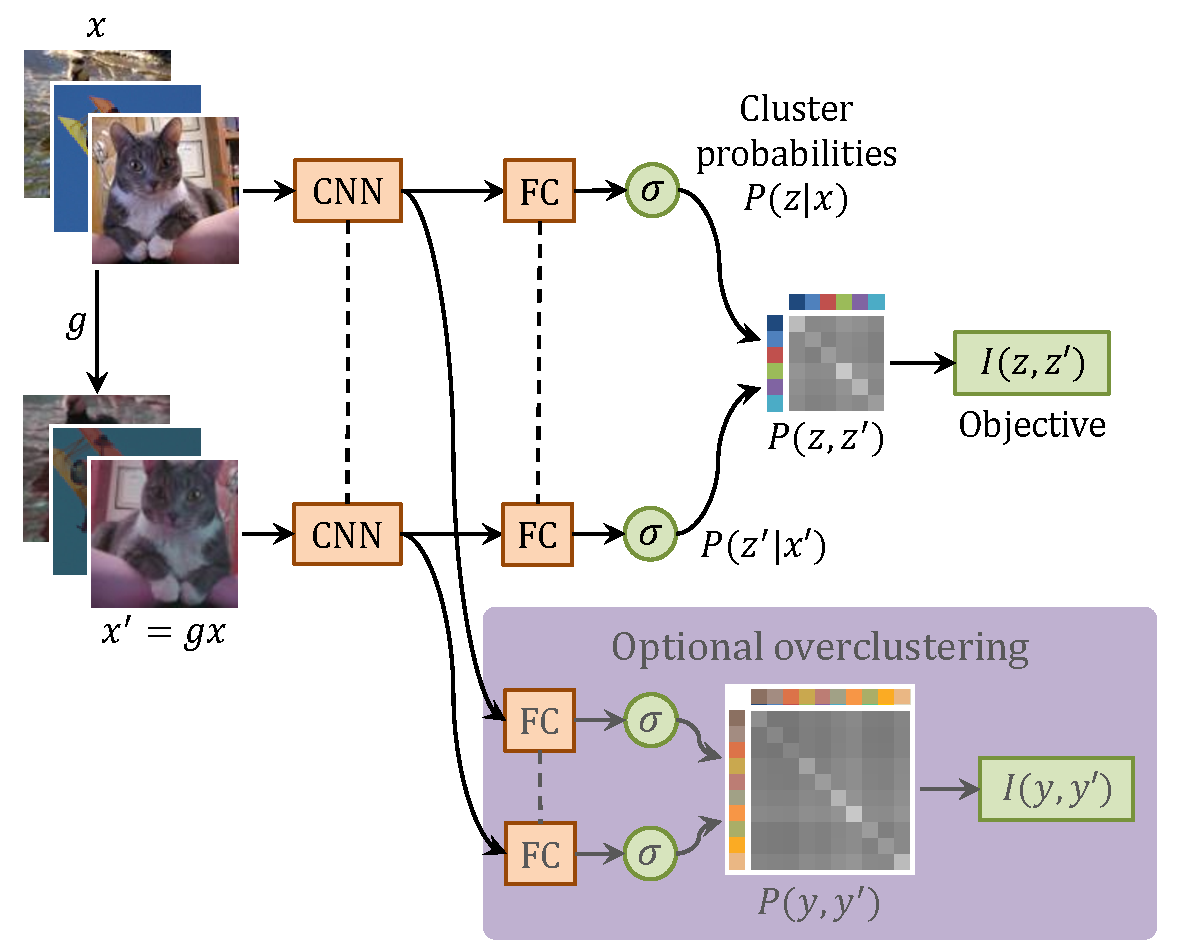
\includegraphics[width=0.95\columnwidth]{paper_imgs/overview1.pdf}
\caption{\label{f:overview}\methodnameshort for image clustering. Dashed line denotes shared parameters, $g$ is a random transformation, and $I$ denotes mutual information~(\cref{e:loss_expanded}).}
\end{figure}


\begin{figure*}
%\captionsetup{justification=centering}
\setlength\tabcolsep{2.2pt} % default value: 6pt

\begin{tabular}{c c c c c c}
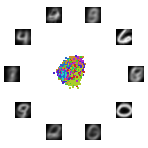
\includegraphics[height=0.16\textwidth]{experiments2_files/mnist_progression/726_run_1_colour_0_pointcloud_0.png} & 
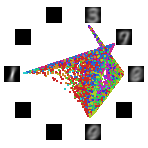
\includegraphics[height=0.16\textwidth]{experiments2_files/mnist_progression/726_run_1_colour_0_pointcloud_3.png} & 
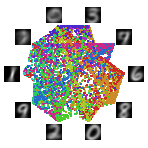
\includegraphics[height=0.16\textwidth]{experiments2_files/mnist_progression/726_run_1_colour_0_pointcloud_10.png} & 
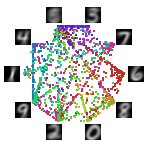
\includegraphics[height=0.16\textwidth]{experiments2_files/mnist_progression/726_run_1_colour_0_pointcloud_30.png} & 
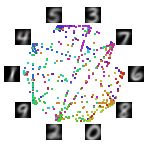
\includegraphics[height=0.16\textwidth]{experiments2_files/mnist_progression/726_run_1_colour_0_pointcloud_101.png} & 
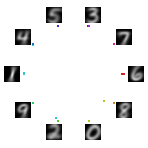
\includegraphics[height=0.16\textwidth]{experiments2_files/mnist_progression/726_run_1_colour_0_pointcloud_1000.png} 
\end{tabular}

\caption{\label{f:mnist_dots} Training with \methodnameshort on unlabelled MNIST in successive epochs from random initialisation (left). The network directly outputs cluster assignment probabilities for input images, and each is rendered as a coordinate by convex combination of 10 cluster vertices. There is no cherry-picking as the entire dataset is shown in every snapshot. Ground truth labelling (unseen by model) is given by colour. At each cluster the average image of its assignees is shown. With neither labels nor heuristics, the clusters discovered by \methodnameshort correspond perfectly to unique digits, with one-hot certain prediction (right).}
\end{figure*}


\paragraph{Co-clustering and mutual information.}

The use of information as a criterion to learn representations is not new. One of the earliest works to do so is by Becker and Hinton~\cite{becker1992self}.
More generally, learning from paired data has been explored in co-clustering~\cite{hartigan1972direct, dhillon2003information} and in other works~\cite{wang2010information} that build on the information bottleneck principle~\cite{friedman2001multivariate}.

Several recent papers have used information as a tool to train deep networks in particular.
IMSAT~\cite{hu2017learning} maximises mutual information between data and its representation and DeepINFOMAX~\cite{hjelm2018learning} maximizes information between spatially-preserved features and compact features.
However, IMSAT and DeepINFOMAX combine information with other criteria, whereas in our method information is the only criterion used.
Furthermore, both IMSAT and DeepINFOMAX compute mutual information over continuous random variables, which requires complex estimators~\cite{belghazi2018mine}, whereas \methodnameshort does so for discrete variables with simple and exact computations.
Finally, DeepINFOMAX considers the information $I(\bx, f(\bx))$ between the features $\bx$ and a deterministic function $f(\bx)$ of it, which is in principle the same as the entropy $H(\bx)$; in contrast, in \methodnameshort information does not trivially reduce to  entropy.

\paragraph{Semantic clustering versus intermediate representation learning.}
In semantic clustering, the learned function directly outputs discrete assignments for high level (i.e. semantic) clusters. Intermediate representation learners, on the other hand, produce continuous, distributed, high-dimensional representations that must be post-processed, for example by k-means, to obtain the discrete low-cardinality assignments required for unsupervised semantic clustering. The latter includes objectives such as generative autoencoder image reconstruction~\cite{vincent2010stacked},  triplets~\cite{schultz2004learning} and spatial-temporal order or context prediction~\cite{lee2017unsupervised,cruz2017deeppermnet,doersch2015unsupervised}, for example predicting patch proximity~\cite{isola2015learning}, solving jigsaw puzzles~\cite{noroozi2016unsupervised} and inpainting~\cite{pathak2016context}. Note it also includes a number of clustering methods (DeepCluster~\cite{caron2018deep}, exemplars~\cite{dosovitskiy2015discriminative}) where the clustering is only auxiliary; a clustering-style objective is used but does not produce groups with semantic correspondence. For example, DeepCluster~\cite{caron2018deep} is a state-of-the-art method for learning highly-transferable intermediate features using overclustering as a proxy task, but does not automatically find semantically meaningful clusters. As these methods use auxiliary objectives divorced from the semantic clustering objective, it is unsurprising that they perform worse than \methodnameshort~(\cref{s:experiments}), which directly optimises for it, training the network end-to-end with the final clusterer implicitly wrapped inside.




\paragraph{Optimising image-to-image distance.}

Many approaches to deep clustering, whether semantic or auxiliary, utilise a distance function between input images that approximates a given grouping criterion.
Agglomerative clustering~\cite{bautista2016cliquecnn} and partially ordered sets~\cite{bautista2017deep} of HOG features~\cite{dalal2005histograms} have been used to group images, and exemplars~\cite{dosovitskiy2015discriminative} define a group as a set of random transformations applied to a single image. Note the latter does not scale easily, in particular to image segmentation where a single $200\times 200$ image would call for 40k classes. DAC~\cite{chang2017deep}, JULE~\cite{yang2016joint}, DeepCluster~\cite{caron2018deep}, ADC~\cite{haeusser2018associative} and DEC~\cite{xie2016unsupervised} rely on the inherent visual consistency and disentangling properties~\cite{greff2015binding} of CNNs to produce cluster assignments, which are processed and reinforced in each iteration. 
The latter three are based on k-means style mechanisms to refine feature centroids, which is prone to degenerate solutions~\cite{caron2018deep} and thus needs explicit prevention mechanisms such as pre-training, cluster-reassignment or feature cleaning via PCA and whitening~\cite{xie2016unsupervised, caron2018deep}.

\begin{comment}
DAC is the only unsupervised clustering algorithm out of these that eschews k-means and agglomerative clustering for a different but similar clustering scheme, based on feature inner-products rather than distances.
DAC forms clusters gradually, in a self-paced manner, thus alleviating but not eliminating the risk of incurring degenerate solutions.
Furthermore, the nature of the optimisation, which reinforces bootstrapped class labels, creates a strong dependency on initialisation.

For unsupervised feature learning in general, i.e.\ where the training objective is not clustering, a large number of works explore using proxy learning tasks. 
There are two major directions:  generative tasks such as autoencoder image reconstruction~\cite{vincent2010stacked}, and spatial-temporal order or context prediction~\cite{lee2017unsupervised,cruz2017deeppermnet,doersch2015unsupervised}. The latter includes predicting patch proximity~\cite{isola2015learning}, solving jigsaw puzzles~\cite{noroozi2016unsupervised} and inpainting~\cite{pathak2016context}. 
In many cases they benefit from principled formulations that protect against degeneracy.
However, unlike the aforementioned clustering methods, the features learned by these methods need to be post-processed, for example using k-means, to cluster the data. 

\end{comment}

\paragraph{Invariance as a training objective.}

Optimising for function outputs to be persistent through spatio-temporal or non-material distortion is an idea shared by \methodnameshort with several works, including exemplars~\cite{dosovitskiy2015discriminative}, IMSAT~\cite{hu2017learning}, proximity prediction~\cite{isola2015learning}, the denoising objective of Tagger~\cite{greff2016tagger}, temporal slowness constraints~\cite{zou2012deep}, and optimising for features to be invariant to local image transformations~\cite{sohn2012learning,hui2013direct}.
More broadly, the problem of modelling data transformation has received significant attention in deep learning, one example being the transforming autoencoder~\cite{hinton2011transforming}.


% \section{Related work}\label{s:related}

% \paragraph{Co-clustering and mutual information.}

% The idea of learning a data representation by seeking the common parts of related observations is not new. 
% An early work is Becker and Hinton~\cite{becker1992self}, which maximises agreement between representations of 2D images to learn depth, using an objective corresponding to maximising mutual information between the input and the average of the data representations. 
% Co-learning has also been explored in the context of clustering by co-clustering methods, dating back to the pioneering work of Hartigan~\cite{hartigan72direct}. 
% Many information-theoretic variant of such approaches have been proposed, as discussed by~\cite{wang10information}, which are generally related to the information bottleneck principle~(\cite{friedman2001multivariate}). 

% A few works have employed mutual information in the context of unsupervised deep learning. IMSAT~\cite{hu2017learning} maximises mutual information between input data and their predicted discrete representations whilst encouraging the representations of augmented data points to be close to those of the original data points. 
% DeepINFOMAX~\cite{hjelm2018learning} maximises mutual information between spatially preserved features and compact features. There are some major differences with \methodnameshort. 
% Firstly, mutual information is used as an aid in these methods, as it increases the statistical predictivity between two random variables. 
% This contrasts with our method, where mutual information constitutes the loss applied directly to cluster assignments, meaning it is used as a clustering objective. 
% Secondly, both IMSAT and DeepINFOMAX compute mutual information over continuous random variables, which calls for an integral and is not computationally tractable, so estimators~\cite{belghazi2018mine} are used. 
% Since \methodnameshort maximises mutual information between cluster assignments and the number of clusters is discrete, computation is exact and straightforward. 
% Finally, DeepINFOMAX employs mutual information between function inputs and outputs, i.e. $I(x, f(x))$, but the conditional entropy component of mutual information $H(f(x) | x)$ is 0 when $f$ is deterministic, making the maximisation less meaningful. 
% In contrast \methodnameshort maximises mutual information between cluster assignments of separate images, i.e. $I(z, z')$ where $z$ and $z'$ are not functions of one other, making $H(z | z')$ a non-zero quantity that contributes to the optimisation as it can be minimised.

% \paragraph{Optimising image-to-image distance for clustering.}
% Many works for on unsupervised deep clustering involve establishing a scheme for estimating the semantic distance between input images, before training a function to learn this scheme. 
% CliqueCNN~\cite{bautista2016cliquecnn} trains a network to discriminate between cliques that are determined by applying agglomerative clustering on image features such as HOG~\cite{dalal2005histograms}. 
% In Exemplar CNNs~\cite{dosovitskiy2016discriminative}, each image and a its set of random transformations is considered a class, and a function is trained to discriminate between these surrogate classes. Like \methodnameshort, this method uses random transformations as a proxy for obtaining images with low semantic distance in the absence of label information. 
% Requiring one class per input image has a large memory footprint which makes Exemplar CNNs infeasible for segmentation (where patches are clustered instead of images, so a single 200x200 image would call for 40k classes). 

% \begin{figure}[t]
\centering
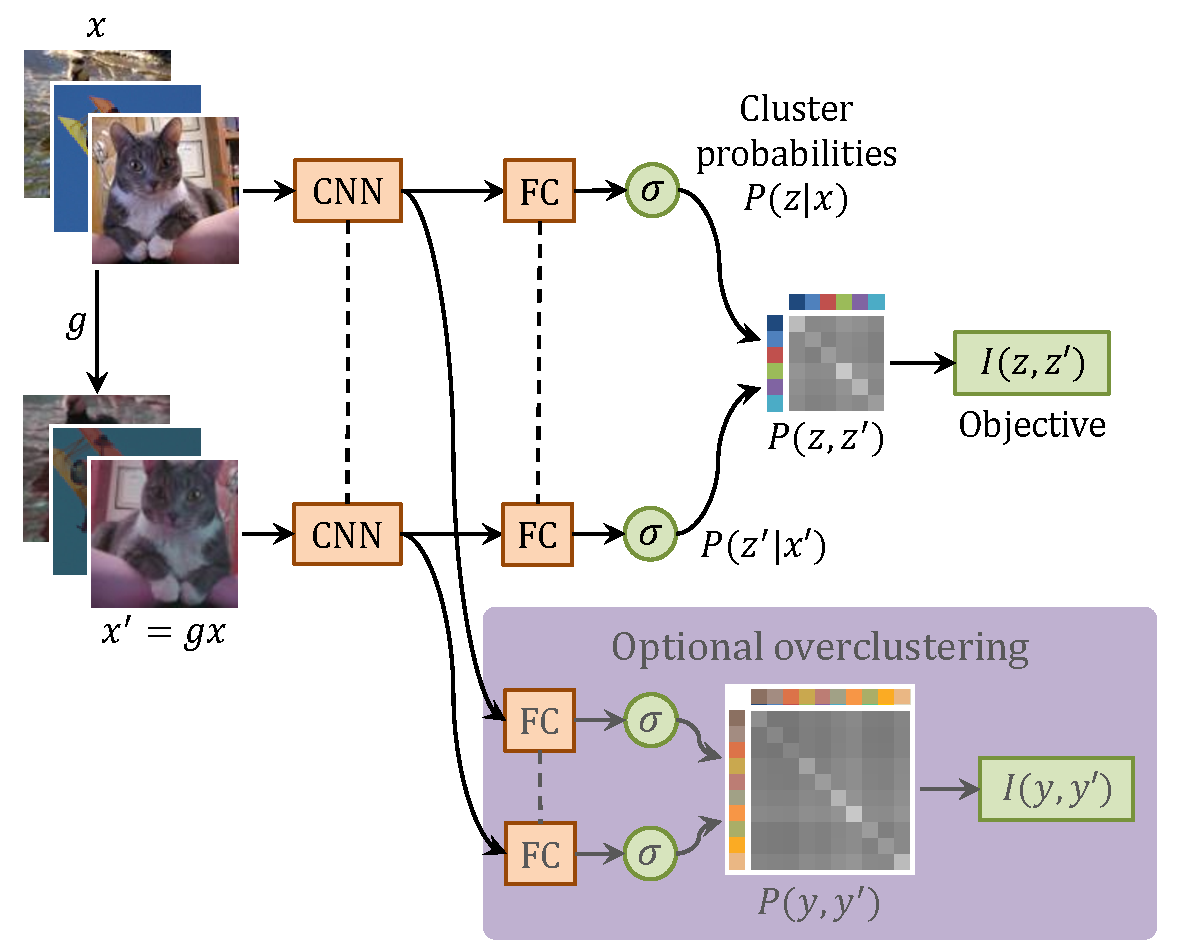
\includegraphics[width=0.95\columnwidth]{paper_imgs/overview1.pdf}
\caption{\label{f:overview}\methodnameshort for image clustering. Dashed line denotes shared parameters, $g$ is a random transformation, and $I$ denotes mutual information~(\cref{e:loss_expanded}).}
\end{figure}


% DAC~\cite{chang2017deep}, JULE~\cite{yang2016joint}, DeepCluster~\cite{caron2018deep}, Associative Deep Clustering~\cite{haeusser18associative} and DEC~\cite{xie2016unsupervised} all rely on the inherent visual consistency and disentangling properties~\cite{greff2015binding} of CNNs to produce meaningful cluster assignments, which are processed and reinforced in each iteration. 
% The latter three are based on using k-means to refine deep feature vectors, a mechanism which is prone to degenerate solutions~\cite{caron2018deep} and thus needs explicit prevention mechanisms such as pre-training, cluster-reassignment or feature cleaning via PCA and whitening ~\cite{xie2016unsupervised, caron2018deep}. 

% DAC is the only unsupervised clustering algorithm out of these that eschews k-means whilst training a network to directly produce cluster assignments, as \methodnameshort does. 
% A network is trained to produce cluster assignment probability distributions for each sample that are used as high level feature descriptors, and the dot product of different descriptors is treated as a proxy for inter-sample semantic distance (instead of Euclidian distance, which is used in the k-means based clusterers). 
% Training proceeds by maximising the dot product of close sample pairs, thus encouraging them to be assigned to the same cluster, whilst minimising the dot product for far pairs. 
% The nature of the optimisation means there is a strong dependency on initialisation and lack of protection against degenerate solutions such as clusters disappearing. 

% \paragraph{Proxy tasks for unsupervised feature learning.}
% For unsupervised feature learning in general, i.e. where the training objective is not clustering, a large number of works explore using proxy learning tasks. 
% There are two major camps:  generative tasks such as autoencoder image reconstruction~\cite{vincent2010stacked}, and spatial-temporal order or context prediction~\cite{lee2017unsupervised,cruz2017deeppermnet,doersch2015unsupervised}. The latter includes predicting patch proximity~\cite{isola2015learning}, solving jigsaw puzzles~(\cite{noroozi2016unsupervised}) and inpainting~(\cite{pathak2016context}). 
% In many cases they benefit from principled formulations that protect against degeneracy.
% However, unlike the aforementioned clustering methods, learned representations from these tasks constitute fine-grained continuous features rather than coarse cluster assignments, and thus must be post-processed, either by unsupervised clustering such as k-means or with label information via SVMs or fine-tuning, in order to produce semantic clusters.

% \paragraph{Invariance as a training objective.}
% Training for function outputs to be persistent through spatio-temporal distortion, noise distortion, or random transforms is an idea shared by \methodnameshort and several mentioned works, including Exemplar CNNs~\cite{dosovitskiy2016discriminative}, IMSAT~\cite{hu2017learning} and proximity prediction~\cite{isola2015learning}.
% It is also seen in Tagger~\cite{greff2016tagger}, which trains a function to denoise its input using several clusters to distribute the representation,~\cite{zou2012deep} which enforces a temporal slowness constraint on learned features, and~\cite{sohn2012learning,hui2013direct} which train for features invariant to local image transformations.



\begin{figure*}
\centering
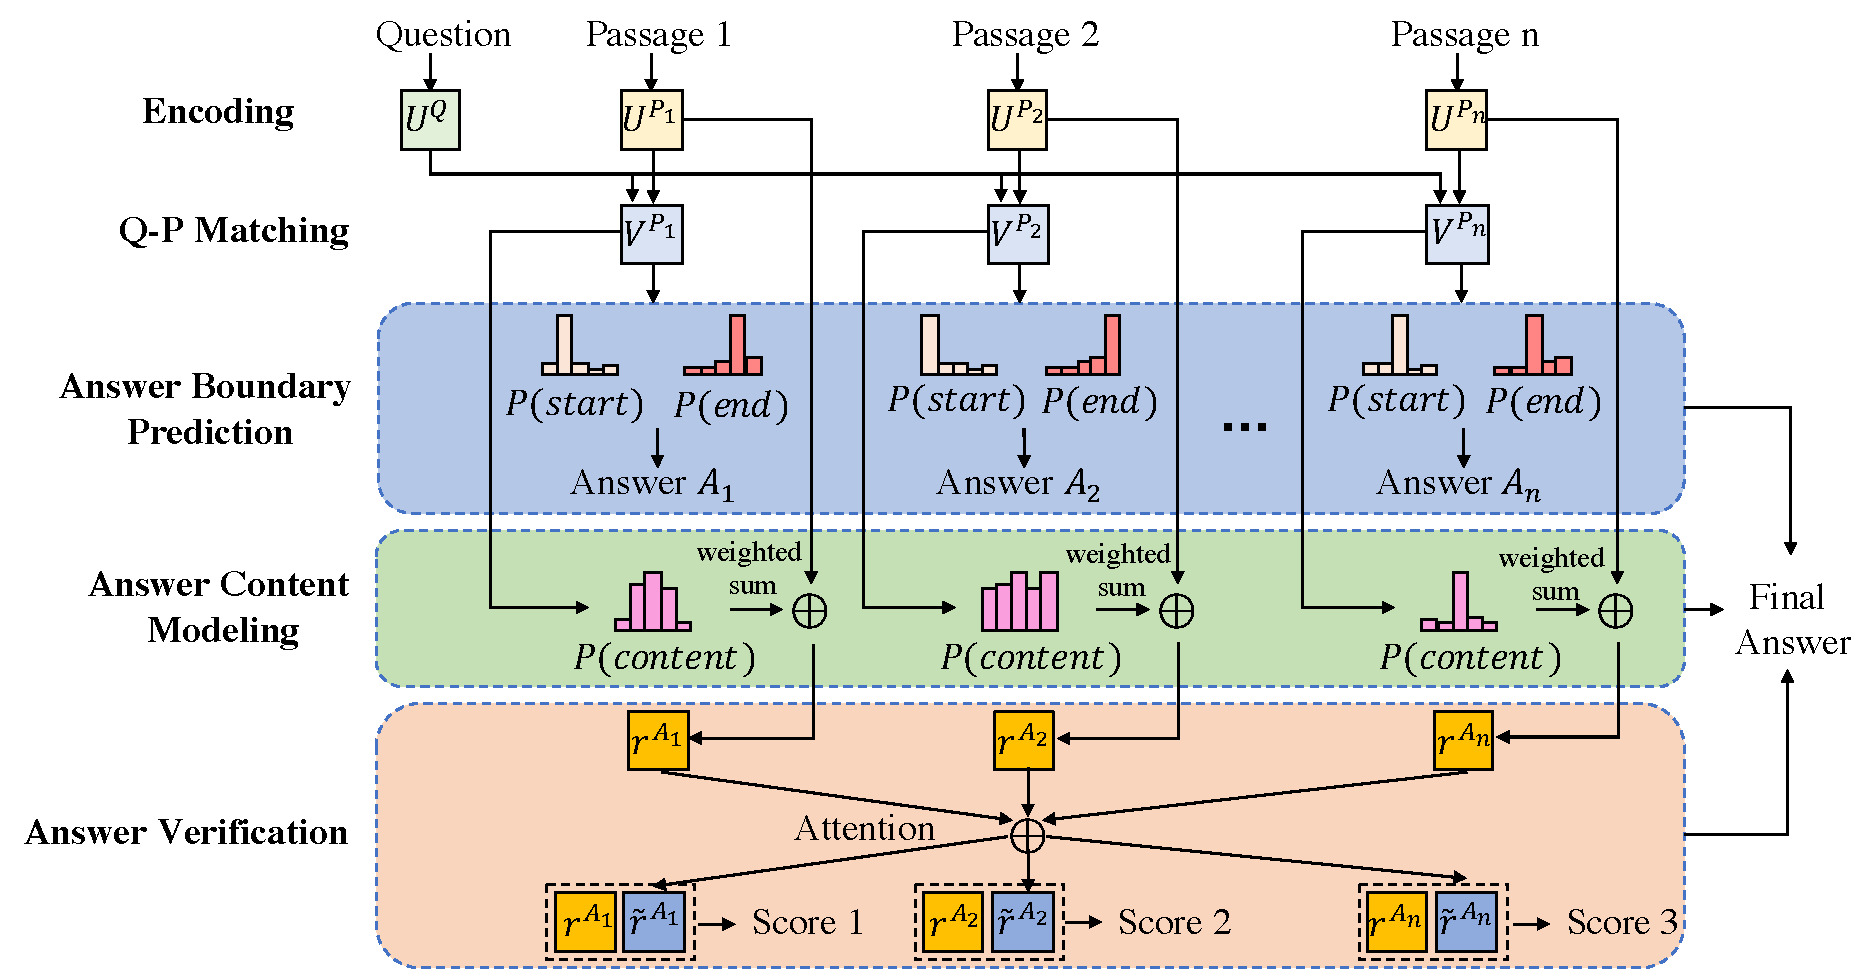
\includegraphics[width=0.85\textwidth]{architecture}
\caption{The overall architecture of our proposed network. The network
contains layers of symmetric convolution (encoder) and deconvolution (decoder).
Skip shortcuts are connected every a few (in our experiments, two) layers from
convolutional feature maps to their mirrored deconvolutional feature maps.
The response from a convolutional layer is directly propagated to the corresponding
mirrored deconvolutional layer, both forwardly and backwardly.}
\label{fig1}
\end{figure*}

\section{Very deep convolutional auto-encoder for image restoration}
\label{sec:main}

The proposed framework mainly contains a chain of convolutional layers and symmetric
deconvolutional layers, as shown in Figure \ref{fig1}. Skip connections are connected
symmetrically from convolutional layers to deconvolutional layers. We term our method
``RED-Net''---very deep Residual Encoder-Decoder Networks.


\subsection{Architecture}

The framework is fully convolutional (and deconvolutional.  Deconvolution is essentially unsampling convolution). Rectification layers are added
after each convolution and deconvolution. For low-level image restoration problems, we
use neither pooling nor unpooling in the network as usually pooling discards useful image
details that are essential for these tasks. It is worth mentioning that since the convolutional
and deconvolutional layers are symmetric, the network is essentially pixel-wise prediction,
thus the size of input image can be arbitrary. The input and output of the network are images
of the same size $w\times h\times c$, where $w$, $h$ and $c$ are width, height and number of channels.

Our main idea is that the convolutional layers act as a feature extractor, which preserve the
primary components of objects in the image and meanwhile eliminating the corruptions.
After forwarding through the convolutional layers, the corrupted input  image is converted into
a ``clean" one. The subtle details of the image contents may be lost during this process.
The deconvolutional layers are then combined to recover the details of image contents.
The output of the deconvolutional layers is the recovered clean version of the input image.
Moreover, we add skip connections  from a convolutional layer to its corresponding
mirrored deconvolutional layer. The passed convolutional feature maps are summed to the
deconvolutional feature maps element-wise, and passed to the next layer after rectification.
Deriving from the above architecture, we have used two networksvin our experiments, which are of 20 layers
 and 30 layers
respectively, for image denoising, image super-resolution, JPEG deblocking and image inpainting.



\subsection{Deconvolution decoder}

Architectures combining layers of convolution and deconvolution~\cite{DBLP:conf/iccv/NohHH15,
hong2015decoupled} have been proposed for semantic segmentation recently. In contrast to
convolutional layers, in which multiple input activations within a filter window are fused
to output a single activation, deconvolutional layers associate a single input activation with
multiple outputs. Deconvolution is usually used as {\em learnable up-sampling layers}.

 In our network,
the convolutional layers successively down-sample the input image content into a  small
size abstraction. Deconvolutional layers then up-sample the abstraction back into its original resolution.

Besides the use of skip connections, a main difference between our model and
~\cite{DBLP:conf/iccv/NohHH15,hong2015decoupled} is that our network is fully convolutional and
deconvolutional, i.e., without pooling and un-pooling. The reason is that for low-level image restoration,
the aim is to eliminate low level corruption while preserving image details instead of learning
image abstractions. Different from high-level applications such as segmentation or recognition,
pooling typically eliminates the abundant image details and can deteriorate restoration performance.



One can simply replace deconvolution with convolution, which results in an architecture that is
very similar to recently proposed very deep fully convolutional neural networks
~\cite{DBLP:conf/cvpr/LongSD15,DBLP:journals/pami/DongLHT16}. However, there exist essential
differences between a fully convolution model and our model. Take image denoising as an example.
We compare the 5-layer and 10-layer fully convolutional network with our network
(combining convolution and deconvolution, but without skip connection). For fully convolutional
networks, we use padding or up-sampling the input to make the input and output be of the same size.
For our network, the first 5 layers are convolutional and the second 5 layers are deconvolutional.
All the other parameters for training are identical, i.e., trained with SGD and learning rate of
$10^{-6}$, noise level $\sigma=70$. The Peak Signal-to-Noise Ratio (PSNR) on the validation set
is reported, which shows that using deconvolution works better than the fully convolutional
counterpart, as shown in Figure \ref{fig2}.


Furthermore, in Figure \ref{fig3}, we visualize some results that are outputs of layer 2, 5, 8 and 10
from the 10-layer fully convolutional network and ours. In the fully convolution case, the noise
is eliminated step by step, i.e., the noise level is reduced after each layer. During this process,
the details of the image content may be lost. Nevertheless, in our network, convolution  preserves
the primary image content. Then deconvolution is used to compensate the details.


\begin{figure}[htb!]
\centering
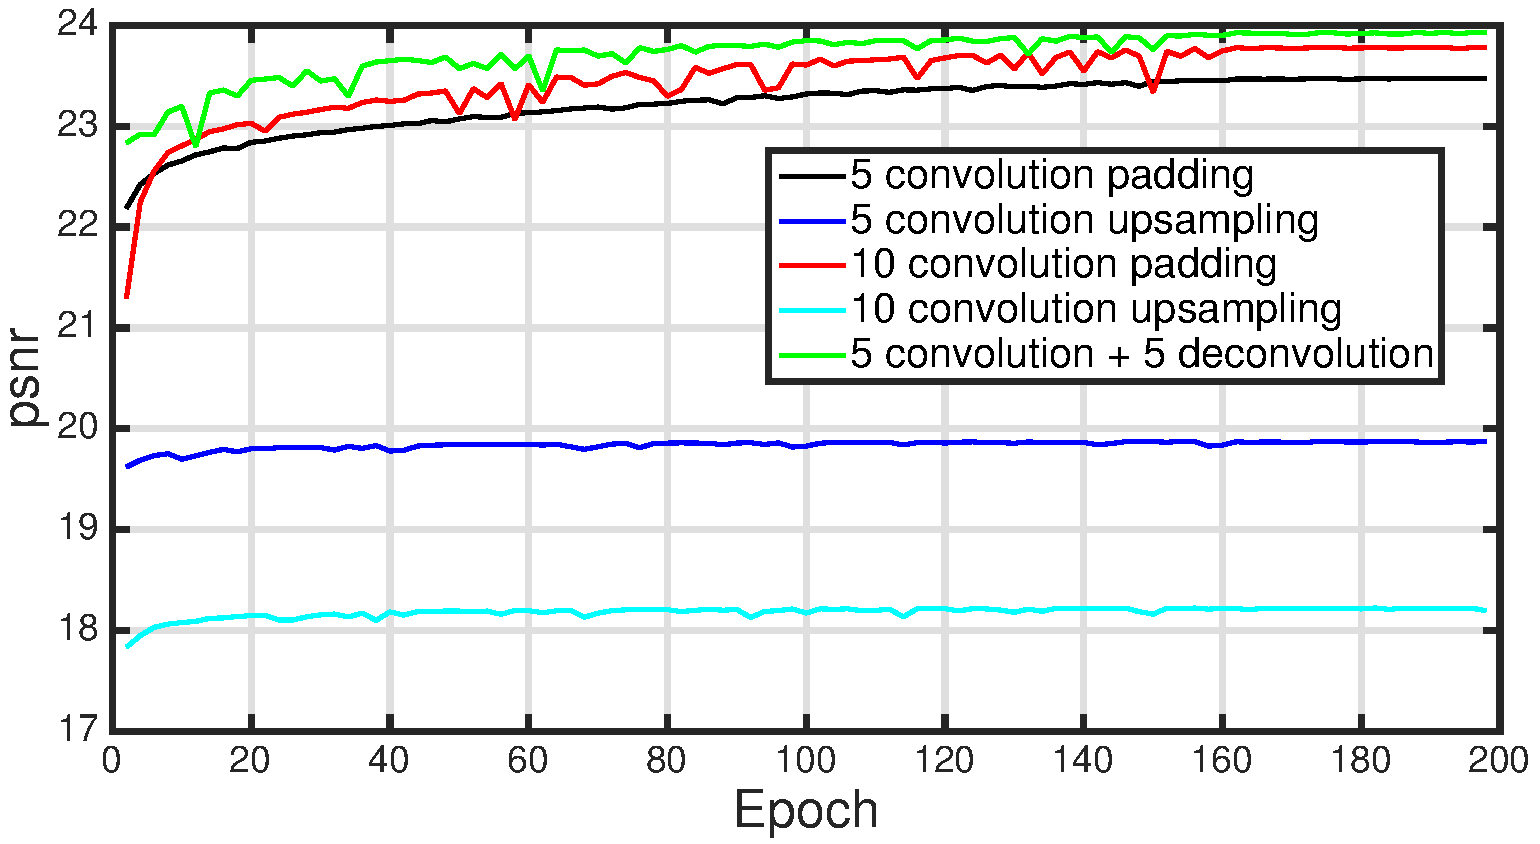
\includegraphics[width=0.48\textwidth]{conv-vs-decv}
\caption{ PSNR  values  on the validation set during training. Our model  exhibits better PSNR
than the compared ones upon convergence.}
\label{fig2}
\end{figure}



\begin{figure}[htb!]
\centering
\subfigure[]{ 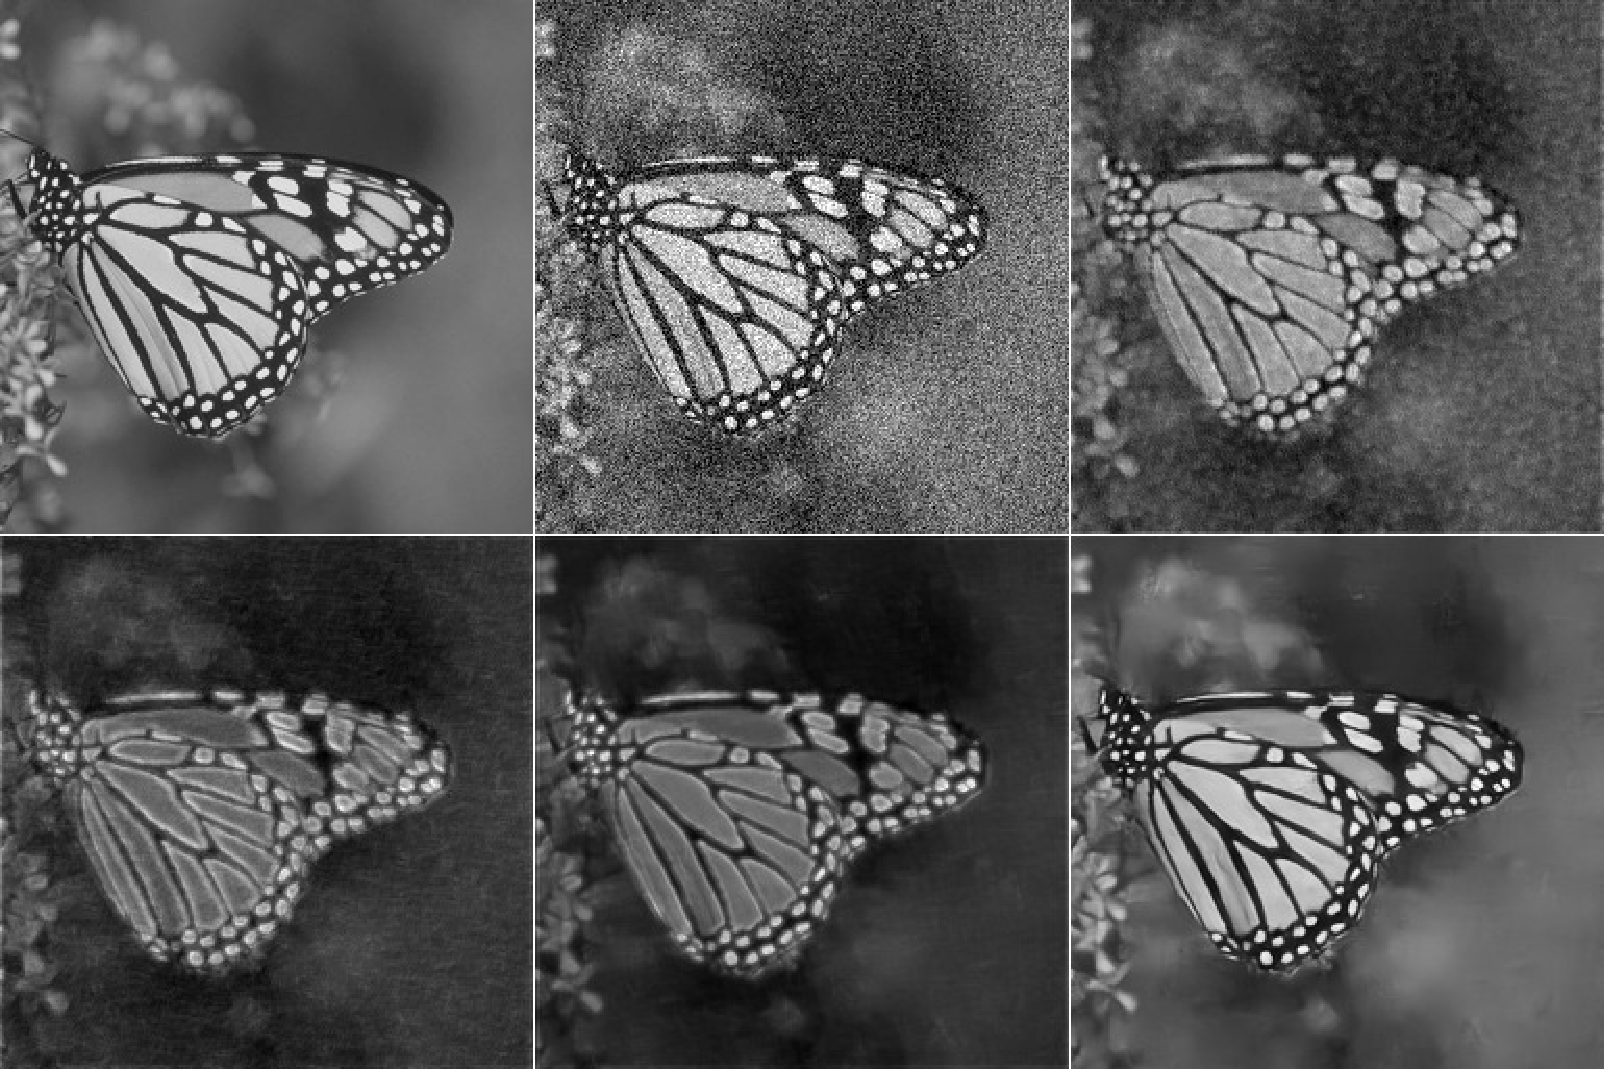
\includegraphics[width=0.48\textwidth]{show-denoising-conv} }
\subfigure[]{ 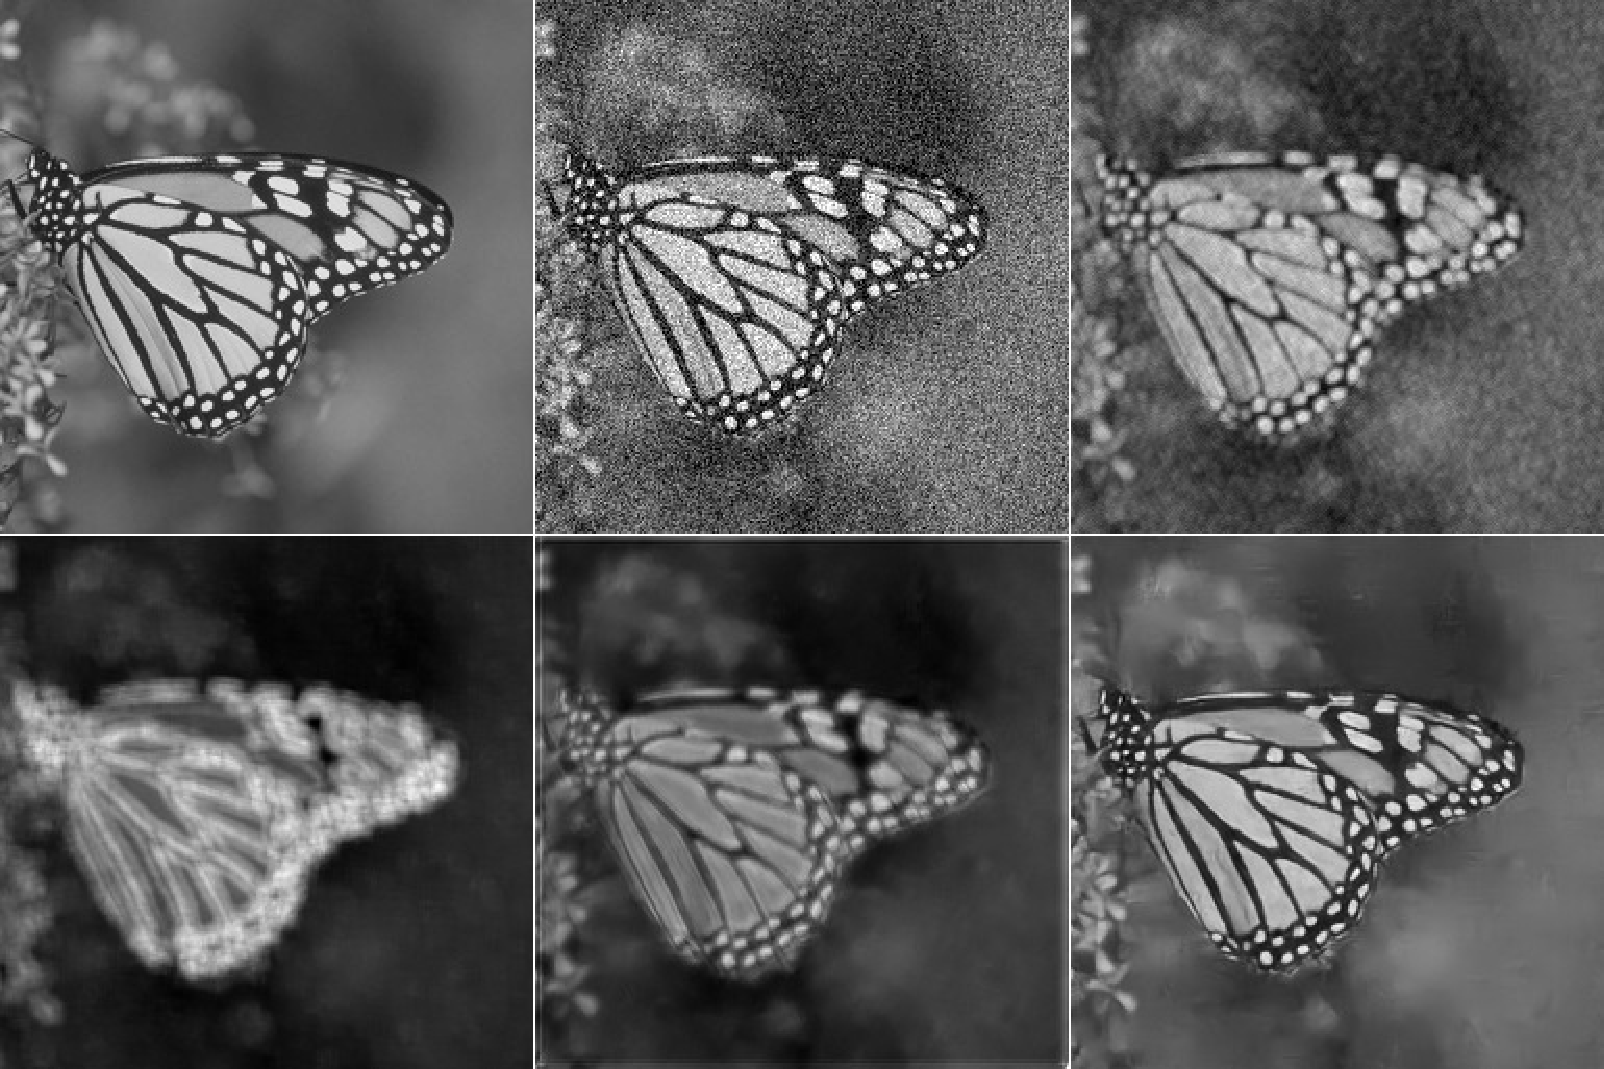
\includegraphics[width=0.48\textwidth]{show-denoising-decv} }
\caption{ (a) Visualization of the 10-layer fully convolutional network. The images from
top-left to bottom-right are: clean image, noisy image, output of conv-2, output of conv-5,
output of conv-8 and output of conv-10, where ``conv-$i$" stands for the $i$-th convolutional layer;
(b) Visualization of the 10-layer convolutional and deconvolutional network. The images from
top-left to bottom-right are: clean image, noisy image, output of conv-2, output of conv-5,
output of deconv-3 and output of deconv-5, where ``deconv-$i$" stands for the $i$-th deconvolutional layer.}
\label{fig3}
\end{figure}




\subsection{Skip connections}

An intuitive question is that, is a network with deconvolution able to recover image details from
the image abstraction only? We find that in shallow networks with only a few layers
of convolution layers, deconvolution is able to recover the details. However, when the
network goes deeper or using operations such as max pooling, even with deconvolution layers, it does not work
that well, possibly because too much details are already lost in the convolution and pooling.


The second question is that, when our network goes deeper, does it achieve performance gain?
We observe that deeper networks in image restoration tasks tend to easily suffer from
performance degradation. The reason may be two folds. First of all, with more layers of
convolution, a significant amount of image details could be lost or corrupted. Given only the image abstraction,
recovering its details is an under-determined problem. Secondly, in terms of optimization,
deep networks often suffer from gradients vanishing and become much harder to train---a problem
that is well addressed in the literature of neural networks.


To address the above two problems, inspired by highway networks \cite{DBLP:journals/corr/SrivastavaGS15}
and deep residual networks \cite{DBLP:journals/corr/HeZRS15}, we add skip connections between
two corresponding convolutional and deconvolutional layers as shown in Figure \ref{fig1}.
A building block is shown in Figure \ref{fig4}. There are two reasons for using such connections.
First, when the network goes deeper, as mentioned above, image details can be lost, making deconvolution
weaker in recovering them. However, the feature maps passed by skip connections carry much image detail,
which helps deconvolution to recover an improved clean version of the image. Second, the skip connections also achieve
benefits on back-propagating the gradient to bottom layers, which makes training deeper network much
easier as observed in \cite{DBLP:journals/corr/SrivastavaGS15} and \cite{DBLP:journals/corr/HeZRS15}.

Note that our skip layer connections are very different from the ones proposed in
\cite{DBLP:journals/corr/SrivastavaGS15} and \cite{DBLP:journals/corr/HeZRS15}, where the only concern
is on the optimization side. In our case, we want to pass information of the convolutional feature maps
to the corresponding deconvolutional layers. The very deep highway networks
\cite{DBLP:journals/corr/SrivastavaGS15} are essentially feedforward long short-term memory (LSTMs)
with forget gates, and the CNN layers of deep residual network \cite{DBLP:journals/corr/HeZRS15}
are feedforward LSTMs without gates. Note that our networks are in general not in the format of
standard feedforward LSTMs.

\begin{figure}[htb!]
\centering
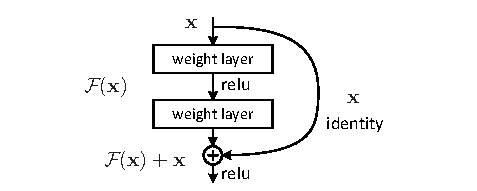
\includegraphics[width=0.48\textwidth]{block}
\caption{An example of a building block in the proposed framework. The rectangle in solid and
dotted lines denote convolution and deconvolution respectively. $\oplus$ denotes element-wise sum of feature maps.}
\label{fig4}
\end{figure}

Instead of directly learning the mappings from the input $X$ to the output $Y$, we would like the network
to fit the residual~\cite{DBLP:journals/corr/HeZRS15} of the problem, which is denoted as $\mathcal{F}(X)=Y-X$.
Such a learning strategy is applied to inner blocks of the encoding-decoding network to make training more
effective. Skip connections are passed every two convolutional layers to their mirrored deconvolutional
layers. Other configurations are possible and our experiments show that this configuration already works
very well. Using such shortcuts makes the network easier to be trained and gains restoration performance
by increasing the network depth.




\subsection{Training}

In general, there are three types of layers in our network: convolution, deconvolution
and element-wise sum. Each layer is followed by a Rectified Linear Unit (ReLU)
~\cite{DBLP:conf/icml/NairH10}. Let $X$ be the input, the convolutional and
deconvolutional layers are expressed as:
\begin{equation}
F(X) = \max(0,W_k * X + B_k),
\end{equation}
where $W_k$ and $B_k$ represent the filters and biases, and $*$ denotes either
convolution or deconvolution operation for the convenience of formulation.
For element-wise sum layer, the output is the element-wise sum of two inputs
of the same size, followed by the ReLU activation:
\begin{equation}
F(X_1,X_2) = \max(0, X_1 + X_2)
\end{equation}

Learning the end-to-end mapping from corrupted images to clean images needs to
estimate the weights $\Theta$ represented by the convolutional and deconvolutional
kernels. Specifically, given a collection of $N$ training sample pairs $\{X^i,Y^i\}$,
where $X^i$ is a noisy image and $Y^i$ is the clean version as the groundtruth.
We minimize the following Mean Squared Error (MSE):
\begin{equation}
  \mathcal{L}(\Theta) = \frac{1}{N}\sum_{i=1}^{N}\|\mathcal{F}(X^i;\Theta)-Y^i\|_F^2.
\label{eq1}
\end{equation}

Traditionally, a  network can learn the mapping from the corrupted image to the clean version
directly. However, our network learns for the additive corruption from the input since there
is a skip connection between the input and the output of the network.
%
%
%
We found that optimizing for the corruption converges better than
optimizing for the clean image. In the extreme case, if the input is a clean image, it would be easier
to push the network to be zero mapping (learning the corruption) than to fit an identity
mapping (learning the clean image) with a stack of nonlinear layers.

We implement and train our network using Caffe~\cite{jia2014caffe}. Empirically, we find
that using Adam~\cite{DBLP:journals/corr/KingmaB14} with base learning rate of $10^{-4}$ for
training converges faster than traditional stochastic gradient descent (SGD). The base
learning rate for all layers are the same, different from ~\cite{DBLP:journals/pami/DongLHT16,
DBLP:conf/nips/JainS08}, in which a smaller learning rate is set for the last layer.
This  is not necessary in our network. Specifically, gradients with respect to the
parameters of $i$th layer is firstly computed as:
\begin{equation}
g = \nabla_{\theta_i}\mathcal{L}(\theta_i).
\end{equation}
Then, the two momentum vectors are computed as:
\begin{equation}
m = \beta_1m + (1 - \beta_1)g,\quad v = \beta_2v + (1-\beta_2)g^2.
\end{equation}
The update rule is:
\begin{equation}
\alpha = \alpha\sqrt{1-\beta_2^t}/(1-\beta_1^t), \quad \theta_i=\theta_i-\alpha m/(\sqrt{v}+\epsilon).
\end{equation}
$\beta_1$, $\beta_2$ and $\epsilon$ are set as the recommended values in~\cite{DBLP:journals/corr/KingmaB14}.

300 images from the Berkeley Segmentation Dataset (BSD)~\cite{MartinFTM01} are used to
generate image patches as the training set for each image restoration task.
%
%
%




\subsection{Testing}

Although trained on local patches, our network can perform restoration on images of arbitrary sizes.
Given a testing image, one can simply go forward through the network, which is already able to
 outperform existing methods. To achieve even better results, we propose
to process a corrupted image on multiple orientations. Different from segmentation, the
filter kernels in our network only eliminate the corruptions, which is usually not sensitive
to the orientation of image contents in low level restoration tasks. Therefore, we can rotate
and mirror flip the kernels and perform forward multiple times, and then average the output to
achieve an ensemble of multiple tests. We see that this can lead to slightly better performance.

\section{Experiments}
\label{sect:experiments}

% \begin{figure*}
%   \centering
%   \setlength{\tabcolsep}{0pt}
%   \setlength\figurewidth{0.05\textwidth}
%   \newcommand{\example}[1]{\raisebox{-.4\height}{\includegraphics[width=\figurewidth]{./figures/domains_examples/#1}}}
%   \begin{sc}
%   \begin{tabular}{r@{\hskip 1cm} ccccccccccc}
%     MNIST \cite{LeCun98} &
%     \example{mnist_0.png} &
%     \example{mnist_1.png} &
%     \example{mnist_2.png} &
%     \example{mnist_3.png} &
%     \example{mnist_4.png} &
%     \example{mnist_5.png} &
%     \example{mnist_6.png} &
%     \example{mnist_7.png} &
%     \example{mnist_8.png} &
%     \example{mnist_9.png} &
%     \example{mnist_10.png}\\
%     MNIST ($ | \Delta | $, BG) &
%     \example{mnisti_0.png} &
%     \example{mnisti_1.png} &
%     \example{mnisti_2.png} &
%     \example{mnisti_3.png} &
%     \example{mnisti_4.png} &
%     \example{mnisti_5.png} &
%     \example{mnisti_6.png} &
%     \example{mnisti_7.png} &
%     \example{mnisti_8.png} &
%     \example{mnisti_9.png} &
%     \example{mnisti_10.png}\\
%     Syn Numbers &
%     \example{syn_0.png} &
%     \example{syn_1.png} &
%     \example{syn_2.png} &
%     \example{syn_3.png} &
%     \example{syn_4.png} &
%     \example{syn_5.png} &
%     \example{syn_6.png} &
%     \example{syn_7.png} &
%     \example{syn_8.png} &
%     \example{syn_9.png} &
%     \example{syn_10.png}\\
%     SVHN \cite{Netzer11} &
%     \example{svhn_0.png} &
%     \example{svhn_1.png} &
%     \example{svhn_2.png} &
%     \example{svhn_3.png} &
%     \example{svhn_4.png} &
%     \example{svhn_5.png} &
%     \example{svhn_6.png} &
%     \example{svhn_7.png} &
%     \example{svhn_8.png} &
%     \example{svhn_9.png} &
%     \example{svhn_10.png}\\
%     Syn Signs &
%     \example{synsgn_11.png} &
%     \example{synsgn_1.png} &
%     \example{synsgn_2.png} &
%     \example{synsgn_3.png} &
%     \example{synsgn_4.png} &
%     \example{synsgn_5.png} &
%     \example{synsgn_12.png} &
%     \example{synsgn_7.png} &
%     \example{synsgn_8.png} &
%     \example{synsgn_9.png} &
%     \example{synsgn_10.png}\\
%     GTSRB \cite{Stallkamp12} &
%     \example{gtsrb_0.png} &
%     \example{gtsrb_1.png} &
%     \example{gtsrb_2.png} &
%     \example{gtsrb_3.png} &
%     \example{gtsrb_4.png} &
%     \example{gtsrb_5.png} &
%     \example{gtsrb_6.png} &
%     \example{gtsrb_7.png} &
%     \example{gtsrb_8.png} &
%     \example{gtsrb_9.png} &
%     \example{gtsrb_10.png}\\
%     % CIFAR-10 \cite{Krizhevsky09} &
%     % \example{cifar10_0.png} &
%     % \example{cifar10_1.png} &
%     % \example{cifar10_2.png} &
%     % \example{cifar10_3.png} &
%     % \example{cifar10_4.png} &
%     % \example{cifar10_5.png} &
%     % \example{cifar10_11.png} &
%     % \example{cifar10_7.png} &
%     % \example{cifar10_8.png} &
%     % \example{cifar10_9.png} &
%     % \example{cifar10_10.png}\\
%     % STL-10 \cite{Coates11} &
%     % \example{stl10_12.png} &
%     % \example{stl10_1.png} &
%     % \example{stl10_2.png} &
%     % \example{stl10_3.png} &
%     % \example{stl10_4.png} &
%     % \example{stl10_5.png} &
%     % \example{stl10_6.png} &
%     % \example{stl10_13.png} &
%     % \example{stl10_8.png} &
%     % \example{stl10_9.png} &
%     % \example{stl10_10.png}\\
%   \end{tabular}
%   \end{sc}
%   \vskip 2.5mm
%   \caption{\todo[What to do with this figure? Add Office? Remove?]Random samples from the datasets used in the experiments. See \sect{exper_quant} for details.}
%   \label{fig:exper_domains_examples}
% \end{figure*}

\begin{figure*}
  \centering
  \setlength{\tabcolsep}{0pt}
  \setlength\figurewidth{0.05\textwidth}
  \newcommand{\example}[1]{\raisebox{-.4\height}{\includegraphics[width=\figurewidth]{./figures/domains_examples/#1}}}
  \begin{sc}
  \begin{small}
  \begin{tabular}{r@{\hskip 0.5cm} ccc c@{\hskip 0.4cm} ccc c@{\hskip 0.4cm} ccc c@{\hskip 0.4cm} ccc}
    &
    \multicolumn{3}{c}{MNIST} & &
    \multicolumn{3}{c}{Syn Numbers} & &
    \multicolumn{3}{c}{SVHN} & &
    \multicolumn{3}{c}{Syn Signs}\\
    
    Source &
    \example{mnist_0.png} &
    \example{mnist_1.png} &
    \example{mnist_3.png} & &
    
    \example{syn_0.png} &
    \example{syn_1.png} &
    \example{syn_2.png} & &
    
    \example{svhn_3.png} &
    \example{svhn_4.png} &
    \example{svhn_5.png} & &
    
    \example{synsgn_3.png} &
    \example{synsgn_4.png} &
    \example{synsgn_5.png}\\
    
    Target &
    \example{mnisti_0.png} &
    \example{mnisti_1.png} &
    \example{mnisti_2.png} & &
    
    \example{svhn_0.png} &
    \example{svhn_1.png} &
    \example{svhn_2.png} & &
    
    \example{mnist_4.png} &
    \example{mnist_5.png} &
    \example{mnist_6.png} & &
    
    \example{gtsrb_2.png} &
    \example{gtsrb_3.png} &
    \example{gtsrb_4.png}\\
    
    &
    \multicolumn{3}{c}{\rule{0pt}{0.35cm} MNIST-M} & &
    \multicolumn{3}{c}{SVHN} & &
    \multicolumn{3}{c}{MNIST} & &
    \multicolumn{3}{c}{GTSRB}\\
  \end{tabular}
  \end{small}
  \end{sc}
  \caption{Examples of domain pairs used in the experiments. See \sect{exper_quant} for details.}
  \label{fig:exper_domains_examples}
\end{figure*}


\begin{table*}[t]
  \vskip 0.15in
  \begin{center}
    \begin{small}
      \begin{sc}
        \renewcommand{\arraystretch}{1.5}
        \begin{tabular}{l r | c c c c}
          \hline
          \multirow{2}{*}{Method} & {\scriptsize Source} & MNIST & Syn Numbers & SVHN & Syn Signs \\
          & {\scriptsize Target} & MNIST-M & SVHN & MNIST & GTSRB \\
          \hline
          \multicolumn{2}{l |}{Source only} & 
          $ .5749 $                      & $ .8665 $                      & $ .5919 $                      & $ .7400 $                      \\
          \multicolumn{2}{l |}{SA \cite{Fernando13}} & 
          $ .6078 \; (7.9\%) $           & $ .8672 \; (1.3\%) $           & $ .6157 \; (5.9\%) $           & $ .7635 \; (9.1\%) $           \\
          \multicolumn{2}{l |}{Proposed approach} & 
          $ \mathbf{.8149} \; (57.9\%) $ & $ \mathbf{.9048} \; (66.1\%) $ & $ \mathbf{.7107} \; (29.3\%) $ & $ \mathbf{.8866} \; (56.7\%) $ \\
          \multicolumn{2}{l |}{Train on target} & 
          $ .9891 $                      & $ .9244 $                      & $ .9951 $                      & $ .9987 $                      \\
          \hline
        \end{tabular}
      \end{sc}
    \end{small}
  \end{center}
    \caption{Classification accuracies for digit image classifications for different source and target domains. {\sc MNIST-M} corresponds to difference-blended digits over non-uniform background. The first row corresponds to the lower performance bound (i.e.\ if no adaptation is performed). The last row corresponds to training on the target domain data with known class labels (upper bound on the DA performance). For each of the two DA methods (ours and \cite{Fernando13}) we show how much of the gap between the lower and the upper bounds was covered (in brackets). For all five cases, our approach outperforms \cite{Fernando13} considerably, and covers a big portion of the gap.\vspace{-0mm} }
  \label{tab:results}
  \vskip -0.1in
\end{table*}

\begin{table*}[t]
  \vskip 0.15in
  \begin{center}
    \begin{small}
      \begin{sc}
        \renewcommand{\arraystretch}{1.5}
        \begin{tabular}{l r | c c c}
          \hline
          \multirow{2}{*}{Method} & {\scriptsize Source} & Amazon & DSLR & Webcam \\
          & {\scriptsize Target} & Webcam & Webcam & DSLR \\
          \hline
          \multicolumn{2}{l |}{GFK(PLS, PCA) \cite{Gong12}} & 
          $ .464 \pm .005 $ & $ .613 \pm .004 $ & $ .663 \pm .004 $\\ 
          \multicolumn{2}{l |}{SA \cite{Fernando13}} & 
          $ .450 $ & $ .648 $ & $ .699 $\\ 
          \multicolumn{2}{l |}{DA-NBNN \cite{Tommasi13}} & 
          $ .528 \pm .037 $ & $ .766 \pm .017 $ & $ .762 \pm .025 $\\ 
          \multicolumn{2}{l |}{DLID \cite{Chopra13}} & 
          $ .519 $ & $ .782 $ & $ .899 $\\
          \multicolumn{2}{l |}{DeCAF$_6$ Source Only \cite{Donahue14}} &
          $ .522 \pm .017 $ & $ .915 \pm .015 $ & --\\ 
          \multicolumn{2}{l |}{DaNN \cite{Ghifary14}} & 
          $ .536 \pm .002 $ & $ .712 \pm .000 $ & $ .835 \pm .000 $\\ 
          \multicolumn{2}{l |}{DDC \cite{Tzeng14}} & 
          $ .594 \pm .008 $ & $ .925 \pm .003 $ & $ .917 \pm .008 $\\ 
          \multicolumn{2}{l |}{Proposed Approach} & 
          $ \mathbf{ .673 \pm .017 } $ & $ \mathbf{ .940 \pm .008 } $ & $ \mathbf{ .937 \pm .010 } $\\
          \hline
        \end{tabular}
      \end{sc}
    \end{small}
  \end{center}
    \caption{Accuracy evaluation of different DA approaches on the standard {\sc Office} \cite{Saenko10} dataset. Our method (last row) outperforms competitors setting the new state-of-the-art.}
  \label{tab:results_office}
\end{table*}

% Other rows refer to the following algorithms (from top to bottom): Geodesic Flow Kernel \cite{Gong12}, Subspace Alignment \cite{Fernando13}, Naive Bayes Nearest Neighbor \cite{Tommasi13},  deep learning approach from \cite{Chopra13}, DeCAF$_6$-features described in \cite{Donahue14}, Domain Adaptive NNs \cite{Ghifary14}, Deep Domain Confusion \cite{Tzeng14}.

\def\X{{\mathbf X}}
\def\y{{\mathbf y}}

% \vspace{2mm}\noindent {\bf Datasets.}
% \label{sect:exper_datasets}

% In order to test our method in the setting of traffic signs classification we obtained~100,000 synthetic images ({\sc Syn~Signs}) simulating various photoshooting conditions. This dataset was used in conjunction with {\it The German Traffic Sign Recognition Benchmark} ({\sc GTSRB}) \cite{Stallkamp12}.

% Finally, we perform domain adaption for the {\sc CIFAR-10} and the {\sc STL-10} downsampled to the size of $ 32 \times 32 $. This pair is considerably different from the previously mentioned datasets as the intra-class variability here is higher.

We perform extensive evaluation of the proposed approach on a number of popular image datasets and their modifications. These include large-scale datasets of small images popular with deep learning methods, and the {\sc Office} datasets \cite{Saenko10}, which are a {\em de facto} standard for domain adaptation in computer vision, but have much fewer images.

\vspace{2mm}\noindent {\bf Baselines.} For the bulk of experiments the following baselines are evaluated. The \textbf{source-only} model is trained without consideration for target-domain data (no domain classifier branch included into the network). The \textbf{train-on-target} model is trained on the target domain with class labels revealed. This model serves as an upper bound on DA methods, assuming that target data are abundant and the shift between the domains is considerable. 

In addition, we compare our approach against the recently proposed unsupervised DA method based on \textbf{subspace alignment (SA)} \cite{Fernando13}, which is simple to setup and test on new datasets, but has also been shown to perform very well in experimental comparisons with other ``shallow'' DA methods. To boost the performance of this baseline, we pick its most important free parameter (the number of principal components) from the range $ \{ 2, \ldots, 60 \} $, so that the test performance on the target domain is maximized. To apply SA in our setting, we train a source-only model and then consider the activations of the last hidden layer in the label predictor (before the final linear classifier) as descriptors/features, and learn the mapping between the source and the target domains \cite{Fernando13}.

Since the SA baseline requires to train a new classifier after adapting the features, and in order to put all the compared settings on an equal footing, we retrain the last layer of the label predictor using a standard linear SVM~\cite{liblinear} for all four considered methods (including ours; the performance on the target domain remains approximately the same after the retraining). 

For the {\sc Office} dataset \cite{Saenko10}, we directly compare the performance of our full network (feature extractor and label predictor) against recent DA approaches using previously published results.

\vspace{2mm}\noindent {\bf CNN architectures.} In general, we compose feature extractor from two or three convolutional layers, picking their exact configurations from previous works. We give the exact architectures in \ref{sect:appendix_archs}.

For the domain adaptator we stick to the three fully connected layers ($x\rightarrow1024\rightarrow1024\rightarrow2$), except for {\sc MNIST} where we used a simpler ($x\rightarrow100\rightarrow2$) architecture to speed up the experiments.

For loss functions, we set $ L_y $ and $ L_d $ to be the logistic regression loss and the binomial cross-entropy respectively.

\vspace{2mm}\noindent {\bf CNN training procedure.}
The model is trained on $128$-sized batches. Images are preprocessed by the mean subtraction. A half of each batch is populated by the samples from the source domain (with known labels), the rest is comprised of the target domain (with unknown labels).

In order to suppress noisy signal from the domain classifier at the early stages of the training procedure instead of fixing the adaptation factor $ \lambda $, we gradually change it from $0$ to $1$ using the following schedule:
\begin{equation}
  \lambda_p = \frac{2}{1 + \exp(-\gamma \cdot p)} - 1,
\end{equation}
where $\gamma$ was set to $10$ in all experiments (the schedule was not optimized/tweaked). Further details on the CNN training can be found in \ref{sect:appendix_training}.

\vspace{2mm}\noindent {\bf Visualizations.}
We use t-SNE \cite{Maaten13} projection to visualize feature distributions at different points of the network, while color-coding the domains (\fig{exper_adapt_vis}). We observe strong correspondence between the success of the adaptation in terms of the classification accuracy for the target domain, and the overlap between the domain distributions in such visualizations.
 
\vspace{2mm}\noindent {\bf Choosing meta-parameters.} 
In general, good unsupervised DA methods should provide ways to set meta-parameters (such as $\lambda$, the learning rate, the momentum rate, the network architecture for our method) in an unsupervised way, i.e.\ without referring to labeled data in the target domain. %Here we would like to give few recommendations concerning this matter. First, as it was pointed out in \sect{theory} the domain classifier should not be significantly more complex than the label predictor. 
In our method, one can assess the performance of the whole system (and the effect of changing hyper-parameters) by observing the test error on the source domain {\em and} the domain classifier error. In general, we observed a good correspondence between the success of adaptation and these errors (adaptation is more successful when the source domain test error is low, while the domain classifier error is high).
In addition, the layer, where the the domain adaptator is attached can be picked by computing difference between means as suggested in \cite{Tzeng14}. 

% \begin{figure*}
%   \centering
%   {\sc MNIST $ \rightarrow $ MNIST ($ | \Delta | $, bg)}: top feature extractor layer
%   \setcounter{subfigure}{0}
%   \subfigure[Non-adapted]{%%
%     \scalebox{0.8}{%% Creator: Matplotlib, PGF backend
%%
%% To include the figure in your LaTeX document, write
%%   \input{<filename>.pgf}
%%
%% Make sure the required packages are loaded in your preamble
%%   \usepackage{pgf}
%%
%% Figures using additional raster images can only be included by \input if
%% they are in the same directory as the main LaTeX file. For loading figures
%% from other directories you can use the `import` package
%%   \usepackage{import}
%% and then include the figures with
%%   \import{<path to file>}{<filename>.pgf}
%%
%% Matplotlib used the following preamble
%%   \usepackage[utf8x]{inputenc}
%%   \usepackage[T1]{fontenc}
%%
\begingroup%
\makeatletter%
\begin{pgfpicture}%
\pgfpathrectangle{\pgfpointorigin}{\pgfqpoint{3.338520in}{2.040000in}}%
\pgfusepath{use as bounding box}%
\begin{pgfscope}%
\pgfsetbuttcap%
\pgfsetroundjoin%
\definecolor{currentfill}{rgb}{1.000000,1.000000,1.000000}%
\pgfsetfillcolor{currentfill}%
\pgfsetlinewidth{0.000000pt}%
\definecolor{currentstroke}{rgb}{1.000000,1.000000,1.000000}%
\pgfsetstrokecolor{currentstroke}%
\pgfsetdash{}{0pt}%
\pgfpathmoveto{\pgfqpoint{0.000000in}{-0.000000in}}%
\pgfpathlineto{\pgfqpoint{3.338520in}{-0.000000in}}%
\pgfpathlineto{\pgfqpoint{3.338520in}{2.040000in}}%
\pgfpathlineto{\pgfqpoint{0.000000in}{2.040000in}}%
\pgfpathclose%
\pgfusepath{fill}%
\end{pgfscope}%
\begin{pgfscope}%
\pgftext[at=\pgfqpoint{0.510000in}{0.348333in},left,bottom]{\pgfimage[interpolate=true,width=2.553333in,height=1.500000in]{./figures/adaptation_vis/pool2_mnist2inv_before-img0.png}}%
\end{pgfscope}%
\begin{pgfscope}%
\pgftext[at=\pgfqpoint{0.805000in}{0.383333in},left,bottom]{\pgfimage[interpolate=true,width=2.201667in,height=1.371667in]{./figures/adaptation_vis/pool2_mnist2inv_before-img1.png}}%
\end{pgfscope}%
\end{pgfpicture}%
\makeatother%
\endgroup%
}}%%
%   \subfigure[Adapted]{%%
%     \scalebox{0.8}{%% Creator: Matplotlib, PGF backend
%%
%% To include the figure in your LaTeX document, write
%%   \input{<filename>.pgf}
%%
%% Make sure the required packages are loaded in your preamble
%%   \usepackage{pgf}
%%
%% Figures using additional raster images can only be included by \input if
%% they are in the same directory as the main LaTeX file. For loading figures
%% from other directories you can use the `import` package
%%   \usepackage{import}
%% and then include the figures with
%%   \import{<path to file>}{<filename>.pgf}
%%
%% Matplotlib used the following preamble
%%   \usepackage[utf8x]{inputenc}
%%   \usepackage[T1]{fontenc}
%%
\begingroup%
\makeatletter%
\begin{pgfpicture}%
\pgfpathrectangle{\pgfpointorigin}{\pgfqpoint{3.340000in}{2.040000in}}%
\pgfusepath{use as bounding box}%
\begin{pgfscope}%
\pgfsetbuttcap%
\pgfsetroundjoin%
\definecolor{currentfill}{rgb}{1.000000,1.000000,1.000000}%
\pgfsetfillcolor{currentfill}%
\pgfsetlinewidth{0.000000pt}%
\definecolor{currentstroke}{rgb}{1.000000,1.000000,1.000000}%
\pgfsetstrokecolor{currentstroke}%
\pgfsetdash{}{0pt}%
\pgfpathmoveto{\pgfqpoint{0.000000in}{-0.000000in}}%
\pgfpathlineto{\pgfqpoint{3.340000in}{-0.000000in}}%
\pgfpathlineto{\pgfqpoint{3.340000in}{2.040000in}}%
\pgfpathlineto{\pgfqpoint{0.000000in}{2.040000in}}%
\pgfpathclose%
\pgfusepath{fill}%
\end{pgfscope}%
\begin{pgfscope}%
\pgftext[at=\pgfqpoint{0.518333in}{0.321667in},left,bottom]{\pgfimage[interpolate=true,width=2.565000in,height=1.550000in]{./figures/adaptation_vis/pool2_mnist2inv_after-img0.png}}%
\end{pgfscope}%
\begin{pgfscope}%
\pgftext[at=\pgfqpoint{0.518333in}{0.321667in},left,bottom]{\pgfimage[interpolate=true,width=2.565000in,height=1.553333in]{./figures/adaptation_vis/pool2_mnist2inv_after-img1.png}}%
\end{pgfscope}%
\end{pgfpicture}%
\makeatother%
\endgroup%
}}\\
%   \vspace{5mm}
%   {\sc Syn Numbers $ \rightarrow $ SVHN}: last hidden layer of the label predictor
%   \setcounter{subfigure}{0}
%   \subfigure[Non-adapted]{%%
%     \scalebox{0.8}{%% Creator: Matplotlib, PGF backend
%%
%% To include the figure in your LaTeX document, write
%%   \input{<filename>.pgf}
%%
%% Make sure the required packages are loaded in your preamble
%%   \usepackage{pgf}
%%
%% Figures using additional raster images can only be included by \input if
%% they are in the same directory as the main LaTeX file. For loading figures
%% from other directories you can use the `import` package
%%   \usepackage{import}
%% and then include the figures with
%%   \import{<path to file>}{<filename>.pgf}
%%
%% Matplotlib used the following preamble
%%   \usepackage[utf8x]{inputenc}
%%   \usepackage[T1]{fontenc}
%%
\begingroup%
\makeatletter%
\begin{pgfpicture}%
\pgfpathrectangle{\pgfpointorigin}{\pgfqpoint{3.340000in}{2.040000in}}%
\pgfusepath{use as bounding box}%
\begin{pgfscope}%
\pgfsetbuttcap%
\pgfsetroundjoin%
\definecolor{currentfill}{rgb}{1.000000,1.000000,1.000000}%
\pgfsetfillcolor{currentfill}%
\pgfsetlinewidth{0.000000pt}%
\definecolor{currentstroke}{rgb}{1.000000,1.000000,1.000000}%
\pgfsetstrokecolor{currentstroke}%
\pgfsetdash{}{0pt}%
\pgfpathmoveto{\pgfqpoint{0.000000in}{-0.000000in}}%
\pgfpathlineto{\pgfqpoint{3.340000in}{-0.000000in}}%
\pgfpathlineto{\pgfqpoint{3.340000in}{2.040000in}}%
\pgfpathlineto{\pgfqpoint{0.000000in}{2.040000in}}%
\pgfpathclose%
\pgfusepath{fill}%
\end{pgfscope}%
\begin{pgfscope}%
\pgftext[at=\pgfqpoint{0.491667in}{0.335000in},left,bottom]{\pgfimage[interpolate=true,width=2.618333in,height=1.531667in]{./figures/adaptation_vis/before-img0.png}}%
\end{pgfscope}%
\begin{pgfscope}%
\pgftext[at=\pgfqpoint{0.758333in}{0.331667in},left,bottom]{\pgfimage[interpolate=true,width=2.171667in,height=1.436667in]{./figures/adaptation_vis/before-img1.png}}%
\end{pgfscope}%
\begin{pgfscope}%
\pgfsetbuttcap%
\pgfsetroundjoin%
\definecolor{currentfill}{rgb}{0.000000,0.000000,1.000000}%
\pgfsetfillcolor{currentfill}%
\pgfsetfillopacity{0.300000}%
\pgfsetlinewidth{0.150562pt}%
\definecolor{currentstroke}{rgb}{0.000000,0.000000,0.000000}%
\pgfsetstrokecolor{currentstroke}%
\pgfsetstrokeopacity{0.300000}%
\pgfsetdash{}{0pt}%
\pgfpathmoveto{\pgfqpoint{2.521160in}{1.775861in}}%
\pgfpathcurveto{\pgfqpoint{2.525278in}{1.775861in}}{\pgfqpoint{2.529228in}{1.777497in}}{\pgfqpoint{2.532140in}{1.780409in}}%
\pgfpathcurveto{\pgfqpoint{2.535052in}{1.783321in}}{\pgfqpoint{2.536688in}{1.787271in}}{\pgfqpoint{2.536688in}{1.791389in}}%
\pgfpathcurveto{\pgfqpoint{2.536688in}{1.795507in}}{\pgfqpoint{2.535052in}{1.799457in}}{\pgfqpoint{2.532140in}{1.802369in}}%
\pgfpathcurveto{\pgfqpoint{2.529228in}{1.805281in}}{\pgfqpoint{2.525278in}{1.806917in}}{\pgfqpoint{2.521160in}{1.806917in}}%
\pgfpathcurveto{\pgfqpoint{2.517042in}{1.806917in}}{\pgfqpoint{2.513092in}{1.805281in}}{\pgfqpoint{2.510180in}{1.802369in}}%
\pgfpathcurveto{\pgfqpoint{2.507268in}{1.799457in}}{\pgfqpoint{2.505631in}{1.795507in}}{\pgfqpoint{2.505631in}{1.791389in}}%
\pgfpathcurveto{\pgfqpoint{2.505631in}{1.787271in}}{\pgfqpoint{2.507268in}{1.783321in}}{\pgfqpoint{2.510180in}{1.780409in}}%
\pgfpathcurveto{\pgfqpoint{2.513092in}{1.777497in}}{\pgfqpoint{2.517042in}{1.775861in}}{\pgfqpoint{2.521160in}{1.775861in}}%
\pgfpathclose%
\pgfusepath{stroke,fill}%
\end{pgfscope}%
\begin{pgfscope}%
\pgfsetbuttcap%
\pgfsetroundjoin%
\definecolor{currentfill}{rgb}{0.000000,0.000000,1.000000}%
\pgfsetfillcolor{currentfill}%
\pgfsetfillopacity{0.300000}%
\pgfsetlinewidth{0.150562pt}%
\definecolor{currentstroke}{rgb}{0.000000,0.000000,0.000000}%
\pgfsetstrokecolor{currentstroke}%
\pgfsetstrokeopacity{0.300000}%
\pgfsetdash{}{0pt}%
\pgfpathmoveto{\pgfqpoint{2.598938in}{1.785583in}}%
\pgfpathcurveto{\pgfqpoint{2.603056in}{1.785583in}}{\pgfqpoint{2.607006in}{1.787219in}}{\pgfqpoint{2.609918in}{1.790131in}}%
\pgfpathcurveto{\pgfqpoint{2.612830in}{1.793043in}}{\pgfqpoint{2.614466in}{1.796993in}}{\pgfqpoint{2.614466in}{1.801111in}}%
\pgfpathcurveto{\pgfqpoint{2.614466in}{1.805229in}}{\pgfqpoint{2.612830in}{1.809179in}}{\pgfqpoint{2.609918in}{1.812091in}}%
\pgfpathcurveto{\pgfqpoint{2.607006in}{1.815003in}}{\pgfqpoint{2.603056in}{1.816639in}}{\pgfqpoint{2.598938in}{1.816639in}}%
\pgfpathcurveto{\pgfqpoint{2.594819in}{1.816639in}}{\pgfqpoint{2.590869in}{1.815003in}}{\pgfqpoint{2.587957in}{1.812091in}}%
\pgfpathcurveto{\pgfqpoint{2.585045in}{1.809179in}}{\pgfqpoint{2.583409in}{1.805229in}}{\pgfqpoint{2.583409in}{1.801111in}}%
\pgfpathcurveto{\pgfqpoint{2.583409in}{1.796993in}}{\pgfqpoint{2.585045in}{1.793043in}}{\pgfqpoint{2.587957in}{1.790131in}}%
\pgfpathcurveto{\pgfqpoint{2.590869in}{1.787219in}}{\pgfqpoint{2.594819in}{1.785583in}}{\pgfqpoint{2.598938in}{1.785583in}}%
\pgfpathclose%
\pgfusepath{stroke,fill}%
\end{pgfscope}%
\begin{pgfscope}%
\pgfsetbuttcap%
\pgfsetroundjoin%
\definecolor{currentfill}{rgb}{0.000000,0.000000,1.000000}%
\pgfsetfillcolor{currentfill}%
\pgfsetfillopacity{0.300000}%
\pgfsetlinewidth{0.150562pt}%
\definecolor{currentstroke}{rgb}{0.000000,0.000000,0.000000}%
\pgfsetstrokecolor{currentstroke}%
\pgfsetstrokeopacity{0.300000}%
\pgfsetdash{}{0pt}%
\pgfpathmoveto{\pgfqpoint{2.676715in}{1.771000in}}%
\pgfpathcurveto{\pgfqpoint{2.680833in}{1.771000in}}{\pgfqpoint{2.684783in}{1.772636in}}{\pgfqpoint{2.687695in}{1.775548in}}%
\pgfpathcurveto{\pgfqpoint{2.690607in}{1.778460in}}{\pgfqpoint{2.692244in}{1.782410in}}{\pgfqpoint{2.692244in}{1.786528in}}%
\pgfpathcurveto{\pgfqpoint{2.692244in}{1.790646in}}{\pgfqpoint{2.690607in}{1.794596in}}{\pgfqpoint{2.687695in}{1.797508in}}%
\pgfpathcurveto{\pgfqpoint{2.684783in}{1.800420in}}{\pgfqpoint{2.680833in}{1.802056in}}{\pgfqpoint{2.676715in}{1.802056in}}%
\pgfpathcurveto{\pgfqpoint{2.672597in}{1.802056in}}{\pgfqpoint{2.668647in}{1.800420in}}{\pgfqpoint{2.665735in}{1.797508in}}%
\pgfpathcurveto{\pgfqpoint{2.662823in}{1.794596in}}{\pgfqpoint{2.661187in}{1.790646in}}{\pgfqpoint{2.661187in}{1.786528in}}%
\pgfpathcurveto{\pgfqpoint{2.661187in}{1.782410in}}{\pgfqpoint{2.662823in}{1.778460in}}{\pgfqpoint{2.665735in}{1.775548in}}%
\pgfpathcurveto{\pgfqpoint{2.668647in}{1.772636in}}{\pgfqpoint{2.672597in}{1.771000in}}{\pgfqpoint{2.676715in}{1.771000in}}%
\pgfpathclose%
\pgfusepath{stroke,fill}%
\end{pgfscope}%
\begin{pgfscope}%
\pgftext[x=2.798938in,y=1.762222in,left,base]{{\rmfamily\fontsize{8.000000}{9.600000}\selectfont Source}}%
\end{pgfscope}%
\begin{pgfscope}%
\pgfsetbuttcap%
\pgfsetroundjoin%
\definecolor{currentfill}{rgb}{1.000000,0.000000,0.000000}%
\pgfsetfillcolor{currentfill}%
\pgfsetfillopacity{0.300000}%
\pgfsetlinewidth{0.150562pt}%
\definecolor{currentstroke}{rgb}{0.000000,0.000000,0.000000}%
\pgfsetstrokecolor{currentstroke}%
\pgfsetstrokeopacity{0.300000}%
\pgfsetdash{}{0pt}%
\pgfpathmoveto{\pgfqpoint{2.521160in}{1.620928in}}%
\pgfpathcurveto{\pgfqpoint{2.525278in}{1.620928in}}{\pgfqpoint{2.529228in}{1.622564in}}{\pgfqpoint{2.532140in}{1.625476in}}%
\pgfpathcurveto{\pgfqpoint{2.535052in}{1.628388in}}{\pgfqpoint{2.536688in}{1.632338in}}{\pgfqpoint{2.536688in}{1.636456in}}%
\pgfpathcurveto{\pgfqpoint{2.536688in}{1.640574in}}{\pgfqpoint{2.535052in}{1.644524in}}{\pgfqpoint{2.532140in}{1.647436in}}%
\pgfpathcurveto{\pgfqpoint{2.529228in}{1.650348in}}{\pgfqpoint{2.525278in}{1.651984in}}{\pgfqpoint{2.521160in}{1.651984in}}%
\pgfpathcurveto{\pgfqpoint{2.517042in}{1.651984in}}{\pgfqpoint{2.513092in}{1.650348in}}{\pgfqpoint{2.510180in}{1.647436in}}%
\pgfpathcurveto{\pgfqpoint{2.507268in}{1.644524in}}{\pgfqpoint{2.505631in}{1.640574in}}{\pgfqpoint{2.505631in}{1.636456in}}%
\pgfpathcurveto{\pgfqpoint{2.505631in}{1.632338in}}{\pgfqpoint{2.507268in}{1.628388in}}{\pgfqpoint{2.510180in}{1.625476in}}%
\pgfpathcurveto{\pgfqpoint{2.513092in}{1.622564in}}{\pgfqpoint{2.517042in}{1.620928in}}{\pgfqpoint{2.521160in}{1.620928in}}%
\pgfpathclose%
\pgfusepath{stroke,fill}%
\end{pgfscope}%
\begin{pgfscope}%
\pgfsetbuttcap%
\pgfsetroundjoin%
\definecolor{currentfill}{rgb}{1.000000,0.000000,0.000000}%
\pgfsetfillcolor{currentfill}%
\pgfsetfillopacity{0.300000}%
\pgfsetlinewidth{0.150562pt}%
\definecolor{currentstroke}{rgb}{0.000000,0.000000,0.000000}%
\pgfsetstrokecolor{currentstroke}%
\pgfsetstrokeopacity{0.300000}%
\pgfsetdash{}{0pt}%
\pgfpathmoveto{\pgfqpoint{2.598938in}{1.630650in}}%
\pgfpathcurveto{\pgfqpoint{2.603056in}{1.630650in}}{\pgfqpoint{2.607006in}{1.632286in}}{\pgfqpoint{2.609918in}{1.635198in}}%
\pgfpathcurveto{\pgfqpoint{2.612830in}{1.638110in}}{\pgfqpoint{2.614466in}{1.642060in}}{\pgfqpoint{2.614466in}{1.646178in}}%
\pgfpathcurveto{\pgfqpoint{2.614466in}{1.650296in}}{\pgfqpoint{2.612830in}{1.654246in}}{\pgfqpoint{2.609918in}{1.657158in}}%
\pgfpathcurveto{\pgfqpoint{2.607006in}{1.660070in}}{\pgfqpoint{2.603056in}{1.661706in}}{\pgfqpoint{2.598938in}{1.661706in}}%
\pgfpathcurveto{\pgfqpoint{2.594819in}{1.661706in}}{\pgfqpoint{2.590869in}{1.660070in}}{\pgfqpoint{2.587957in}{1.657158in}}%
\pgfpathcurveto{\pgfqpoint{2.585045in}{1.654246in}}{\pgfqpoint{2.583409in}{1.650296in}}{\pgfqpoint{2.583409in}{1.646178in}}%
\pgfpathcurveto{\pgfqpoint{2.583409in}{1.642060in}}{\pgfqpoint{2.585045in}{1.638110in}}{\pgfqpoint{2.587957in}{1.635198in}}%
\pgfpathcurveto{\pgfqpoint{2.590869in}{1.632286in}}{\pgfqpoint{2.594819in}{1.630650in}}{\pgfqpoint{2.598938in}{1.630650in}}%
\pgfpathclose%
\pgfusepath{stroke,fill}%
\end{pgfscope}%
\begin{pgfscope}%
\pgfsetbuttcap%
\pgfsetroundjoin%
\definecolor{currentfill}{rgb}{1.000000,0.000000,0.000000}%
\pgfsetfillcolor{currentfill}%
\pgfsetfillopacity{0.300000}%
\pgfsetlinewidth{0.150562pt}%
\definecolor{currentstroke}{rgb}{0.000000,0.000000,0.000000}%
\pgfsetstrokecolor{currentstroke}%
\pgfsetstrokeopacity{0.300000}%
\pgfsetdash{}{0pt}%
\pgfpathmoveto{\pgfqpoint{2.676715in}{1.616066in}}%
\pgfpathcurveto{\pgfqpoint{2.680833in}{1.616066in}}{\pgfqpoint{2.684783in}{1.617703in}}{\pgfqpoint{2.687695in}{1.620615in}}%
\pgfpathcurveto{\pgfqpoint{2.690607in}{1.623527in}}{\pgfqpoint{2.692244in}{1.627477in}}{\pgfqpoint{2.692244in}{1.631595in}}%
\pgfpathcurveto{\pgfqpoint{2.692244in}{1.635713in}}{\pgfqpoint{2.690607in}{1.639663in}}{\pgfqpoint{2.687695in}{1.642575in}}%
\pgfpathcurveto{\pgfqpoint{2.684783in}{1.645487in}}{\pgfqpoint{2.680833in}{1.647123in}}{\pgfqpoint{2.676715in}{1.647123in}}%
\pgfpathcurveto{\pgfqpoint{2.672597in}{1.647123in}}{\pgfqpoint{2.668647in}{1.645487in}}{\pgfqpoint{2.665735in}{1.642575in}}%
\pgfpathcurveto{\pgfqpoint{2.662823in}{1.639663in}}{\pgfqpoint{2.661187in}{1.635713in}}{\pgfqpoint{2.661187in}{1.631595in}}%
\pgfpathcurveto{\pgfqpoint{2.661187in}{1.627477in}}{\pgfqpoint{2.662823in}{1.623527in}}{\pgfqpoint{2.665735in}{1.620615in}}%
\pgfpathcurveto{\pgfqpoint{2.668647in}{1.617703in}}{\pgfqpoint{2.672597in}{1.616066in}}{\pgfqpoint{2.676715in}{1.616066in}}%
\pgfpathclose%
\pgfusepath{stroke,fill}%
\end{pgfscope}%
\begin{pgfscope}%
\pgftext[x=2.798938in,y=1.607289in,left,base]{{\rmfamily\fontsize{8.000000}{9.600000}\selectfont Target}}%
\end{pgfscope}%
\end{pgfpicture}%
\makeatother%
\endgroup%
}}%%
%   \subfigure[Adapted]{%%
%     \scalebox{0.8}{%% Creator: Matplotlib, PGF backend
%%
%% To include the figure in your LaTeX document, write
%%   \input{<filename>.pgf}
%%
%% Make sure the required packages are loaded in your preamble
%%   \usepackage{pgf}
%%
%% Figures using additional raster images can only be included by \input if
%% they are in the same directory as the main LaTeX file. For loading figures
%% from other directories you can use the `import` package
%%   \usepackage{import}
%% and then include the figures with
%%   \import{<path to file>}{<filename>.pgf}
%%
%% Matplotlib used the following preamble
%%   \usepackage[utf8x]{inputenc}
%%   \usepackage[T1]{fontenc}
%%
\begingroup%
\makeatletter%
\begin{pgfpicture}%
\pgfpathrectangle{\pgfpointorigin}{\pgfqpoint{3.340000in}{2.040000in}}%
\pgfusepath{use as bounding box}%
\begin{pgfscope}%
\pgfsetbuttcap%
\pgfsetroundjoin%
\definecolor{currentfill}{rgb}{1.000000,1.000000,1.000000}%
\pgfsetfillcolor{currentfill}%
\pgfsetlinewidth{0.000000pt}%
\definecolor{currentstroke}{rgb}{1.000000,1.000000,1.000000}%
\pgfsetstrokecolor{currentstroke}%
\pgfsetdash{}{0pt}%
\pgfpathmoveto{\pgfqpoint{0.000000in}{-0.000000in}}%
\pgfpathlineto{\pgfqpoint{3.340000in}{-0.000000in}}%
\pgfpathlineto{\pgfqpoint{3.340000in}{2.040000in}}%
\pgfpathlineto{\pgfqpoint{0.000000in}{2.040000in}}%
\pgfpathclose%
\pgfusepath{fill}%
\end{pgfscope}%
\begin{pgfscope}%
\pgftext[at=\pgfqpoint{0.501667in}{0.330000in},left,bottom]{\pgfimage[interpolate=true,width=2.600000in,height=1.540000in]{./figures/adaptation_vis/after-img0.png}}%
\end{pgfscope}%
\begin{pgfscope}%
\pgftext[at=\pgfqpoint{0.500000in}{0.320000in},left,bottom]{\pgfimage[interpolate=true,width=2.585000in,height=1.556667in]{./figures/adaptation_vis/after-img1.png}}%
\end{pgfscope}%
\begin{pgfscope}%
\pgfsetbuttcap%
\pgfsetroundjoin%
\definecolor{currentfill}{rgb}{0.000000,0.000000,1.000000}%
\pgfsetfillcolor{currentfill}%
\pgfsetfillopacity{0.300000}%
\pgfsetlinewidth{0.150562pt}%
\definecolor{currentstroke}{rgb}{0.000000,0.000000,0.000000}%
\pgfsetstrokecolor{currentstroke}%
\pgfsetstrokeopacity{0.300000}%
\pgfsetdash{}{0pt}%
\pgfpathmoveto{\pgfqpoint{2.521160in}{1.775861in}}%
\pgfpathcurveto{\pgfqpoint{2.525278in}{1.775861in}}{\pgfqpoint{2.529228in}{1.777497in}}{\pgfqpoint{2.532140in}{1.780409in}}%
\pgfpathcurveto{\pgfqpoint{2.535052in}{1.783321in}}{\pgfqpoint{2.536688in}{1.787271in}}{\pgfqpoint{2.536688in}{1.791389in}}%
\pgfpathcurveto{\pgfqpoint{2.536688in}{1.795507in}}{\pgfqpoint{2.535052in}{1.799457in}}{\pgfqpoint{2.532140in}{1.802369in}}%
\pgfpathcurveto{\pgfqpoint{2.529228in}{1.805281in}}{\pgfqpoint{2.525278in}{1.806917in}}{\pgfqpoint{2.521160in}{1.806917in}}%
\pgfpathcurveto{\pgfqpoint{2.517042in}{1.806917in}}{\pgfqpoint{2.513092in}{1.805281in}}{\pgfqpoint{2.510180in}{1.802369in}}%
\pgfpathcurveto{\pgfqpoint{2.507268in}{1.799457in}}{\pgfqpoint{2.505631in}{1.795507in}}{\pgfqpoint{2.505631in}{1.791389in}}%
\pgfpathcurveto{\pgfqpoint{2.505631in}{1.787271in}}{\pgfqpoint{2.507268in}{1.783321in}}{\pgfqpoint{2.510180in}{1.780409in}}%
\pgfpathcurveto{\pgfqpoint{2.513092in}{1.777497in}}{\pgfqpoint{2.517042in}{1.775861in}}{\pgfqpoint{2.521160in}{1.775861in}}%
\pgfpathclose%
\pgfusepath{stroke,fill}%
\end{pgfscope}%
\begin{pgfscope}%
\pgfsetbuttcap%
\pgfsetroundjoin%
\definecolor{currentfill}{rgb}{0.000000,0.000000,1.000000}%
\pgfsetfillcolor{currentfill}%
\pgfsetfillopacity{0.300000}%
\pgfsetlinewidth{0.150562pt}%
\definecolor{currentstroke}{rgb}{0.000000,0.000000,0.000000}%
\pgfsetstrokecolor{currentstroke}%
\pgfsetstrokeopacity{0.300000}%
\pgfsetdash{}{0pt}%
\pgfpathmoveto{\pgfqpoint{2.598938in}{1.785583in}}%
\pgfpathcurveto{\pgfqpoint{2.603056in}{1.785583in}}{\pgfqpoint{2.607006in}{1.787219in}}{\pgfqpoint{2.609918in}{1.790131in}}%
\pgfpathcurveto{\pgfqpoint{2.612830in}{1.793043in}}{\pgfqpoint{2.614466in}{1.796993in}}{\pgfqpoint{2.614466in}{1.801111in}}%
\pgfpathcurveto{\pgfqpoint{2.614466in}{1.805229in}}{\pgfqpoint{2.612830in}{1.809179in}}{\pgfqpoint{2.609918in}{1.812091in}}%
\pgfpathcurveto{\pgfqpoint{2.607006in}{1.815003in}}{\pgfqpoint{2.603056in}{1.816639in}}{\pgfqpoint{2.598938in}{1.816639in}}%
\pgfpathcurveto{\pgfqpoint{2.594819in}{1.816639in}}{\pgfqpoint{2.590869in}{1.815003in}}{\pgfqpoint{2.587957in}{1.812091in}}%
\pgfpathcurveto{\pgfqpoint{2.585045in}{1.809179in}}{\pgfqpoint{2.583409in}{1.805229in}}{\pgfqpoint{2.583409in}{1.801111in}}%
\pgfpathcurveto{\pgfqpoint{2.583409in}{1.796993in}}{\pgfqpoint{2.585045in}{1.793043in}}{\pgfqpoint{2.587957in}{1.790131in}}%
\pgfpathcurveto{\pgfqpoint{2.590869in}{1.787219in}}{\pgfqpoint{2.594819in}{1.785583in}}{\pgfqpoint{2.598938in}{1.785583in}}%
\pgfpathclose%
\pgfusepath{stroke,fill}%
\end{pgfscope}%
\begin{pgfscope}%
\pgfsetbuttcap%
\pgfsetroundjoin%
\definecolor{currentfill}{rgb}{0.000000,0.000000,1.000000}%
\pgfsetfillcolor{currentfill}%
\pgfsetfillopacity{0.300000}%
\pgfsetlinewidth{0.150562pt}%
\definecolor{currentstroke}{rgb}{0.000000,0.000000,0.000000}%
\pgfsetstrokecolor{currentstroke}%
\pgfsetstrokeopacity{0.300000}%
\pgfsetdash{}{0pt}%
\pgfpathmoveto{\pgfqpoint{2.676715in}{1.771000in}}%
\pgfpathcurveto{\pgfqpoint{2.680833in}{1.771000in}}{\pgfqpoint{2.684783in}{1.772636in}}{\pgfqpoint{2.687695in}{1.775548in}}%
\pgfpathcurveto{\pgfqpoint{2.690607in}{1.778460in}}{\pgfqpoint{2.692244in}{1.782410in}}{\pgfqpoint{2.692244in}{1.786528in}}%
\pgfpathcurveto{\pgfqpoint{2.692244in}{1.790646in}}{\pgfqpoint{2.690607in}{1.794596in}}{\pgfqpoint{2.687695in}{1.797508in}}%
\pgfpathcurveto{\pgfqpoint{2.684783in}{1.800420in}}{\pgfqpoint{2.680833in}{1.802056in}}{\pgfqpoint{2.676715in}{1.802056in}}%
\pgfpathcurveto{\pgfqpoint{2.672597in}{1.802056in}}{\pgfqpoint{2.668647in}{1.800420in}}{\pgfqpoint{2.665735in}{1.797508in}}%
\pgfpathcurveto{\pgfqpoint{2.662823in}{1.794596in}}{\pgfqpoint{2.661187in}{1.790646in}}{\pgfqpoint{2.661187in}{1.786528in}}%
\pgfpathcurveto{\pgfqpoint{2.661187in}{1.782410in}}{\pgfqpoint{2.662823in}{1.778460in}}{\pgfqpoint{2.665735in}{1.775548in}}%
\pgfpathcurveto{\pgfqpoint{2.668647in}{1.772636in}}{\pgfqpoint{2.672597in}{1.771000in}}{\pgfqpoint{2.676715in}{1.771000in}}%
\pgfpathclose%
\pgfusepath{stroke,fill}%
\end{pgfscope}%
\begin{pgfscope}%
\pgftext[x=2.798938in,y=1.762222in,left,base]{{\rmfamily\fontsize{8.000000}{9.600000}\selectfont Source}}%
\end{pgfscope}%
\begin{pgfscope}%
\pgfsetbuttcap%
\pgfsetroundjoin%
\definecolor{currentfill}{rgb}{1.000000,0.000000,0.000000}%
\pgfsetfillcolor{currentfill}%
\pgfsetfillopacity{0.300000}%
\pgfsetlinewidth{0.150562pt}%
\definecolor{currentstroke}{rgb}{0.000000,0.000000,0.000000}%
\pgfsetstrokecolor{currentstroke}%
\pgfsetstrokeopacity{0.300000}%
\pgfsetdash{}{0pt}%
\pgfpathmoveto{\pgfqpoint{2.521160in}{1.620928in}}%
\pgfpathcurveto{\pgfqpoint{2.525278in}{1.620928in}}{\pgfqpoint{2.529228in}{1.622564in}}{\pgfqpoint{2.532140in}{1.625476in}}%
\pgfpathcurveto{\pgfqpoint{2.535052in}{1.628388in}}{\pgfqpoint{2.536688in}{1.632338in}}{\pgfqpoint{2.536688in}{1.636456in}}%
\pgfpathcurveto{\pgfqpoint{2.536688in}{1.640574in}}{\pgfqpoint{2.535052in}{1.644524in}}{\pgfqpoint{2.532140in}{1.647436in}}%
\pgfpathcurveto{\pgfqpoint{2.529228in}{1.650348in}}{\pgfqpoint{2.525278in}{1.651984in}}{\pgfqpoint{2.521160in}{1.651984in}}%
\pgfpathcurveto{\pgfqpoint{2.517042in}{1.651984in}}{\pgfqpoint{2.513092in}{1.650348in}}{\pgfqpoint{2.510180in}{1.647436in}}%
\pgfpathcurveto{\pgfqpoint{2.507268in}{1.644524in}}{\pgfqpoint{2.505631in}{1.640574in}}{\pgfqpoint{2.505631in}{1.636456in}}%
\pgfpathcurveto{\pgfqpoint{2.505631in}{1.632338in}}{\pgfqpoint{2.507268in}{1.628388in}}{\pgfqpoint{2.510180in}{1.625476in}}%
\pgfpathcurveto{\pgfqpoint{2.513092in}{1.622564in}}{\pgfqpoint{2.517042in}{1.620928in}}{\pgfqpoint{2.521160in}{1.620928in}}%
\pgfpathclose%
\pgfusepath{stroke,fill}%
\end{pgfscope}%
\begin{pgfscope}%
\pgfsetbuttcap%
\pgfsetroundjoin%
\definecolor{currentfill}{rgb}{1.000000,0.000000,0.000000}%
\pgfsetfillcolor{currentfill}%
\pgfsetfillopacity{0.300000}%
\pgfsetlinewidth{0.150562pt}%
\definecolor{currentstroke}{rgb}{0.000000,0.000000,0.000000}%
\pgfsetstrokecolor{currentstroke}%
\pgfsetstrokeopacity{0.300000}%
\pgfsetdash{}{0pt}%
\pgfpathmoveto{\pgfqpoint{2.598938in}{1.630650in}}%
\pgfpathcurveto{\pgfqpoint{2.603056in}{1.630650in}}{\pgfqpoint{2.607006in}{1.632286in}}{\pgfqpoint{2.609918in}{1.635198in}}%
\pgfpathcurveto{\pgfqpoint{2.612830in}{1.638110in}}{\pgfqpoint{2.614466in}{1.642060in}}{\pgfqpoint{2.614466in}{1.646178in}}%
\pgfpathcurveto{\pgfqpoint{2.614466in}{1.650296in}}{\pgfqpoint{2.612830in}{1.654246in}}{\pgfqpoint{2.609918in}{1.657158in}}%
\pgfpathcurveto{\pgfqpoint{2.607006in}{1.660070in}}{\pgfqpoint{2.603056in}{1.661706in}}{\pgfqpoint{2.598938in}{1.661706in}}%
\pgfpathcurveto{\pgfqpoint{2.594819in}{1.661706in}}{\pgfqpoint{2.590869in}{1.660070in}}{\pgfqpoint{2.587957in}{1.657158in}}%
\pgfpathcurveto{\pgfqpoint{2.585045in}{1.654246in}}{\pgfqpoint{2.583409in}{1.650296in}}{\pgfqpoint{2.583409in}{1.646178in}}%
\pgfpathcurveto{\pgfqpoint{2.583409in}{1.642060in}}{\pgfqpoint{2.585045in}{1.638110in}}{\pgfqpoint{2.587957in}{1.635198in}}%
\pgfpathcurveto{\pgfqpoint{2.590869in}{1.632286in}}{\pgfqpoint{2.594819in}{1.630650in}}{\pgfqpoint{2.598938in}{1.630650in}}%
\pgfpathclose%
\pgfusepath{stroke,fill}%
\end{pgfscope}%
\begin{pgfscope}%
\pgfsetbuttcap%
\pgfsetroundjoin%
\definecolor{currentfill}{rgb}{1.000000,0.000000,0.000000}%
\pgfsetfillcolor{currentfill}%
\pgfsetfillopacity{0.300000}%
\pgfsetlinewidth{0.150562pt}%
\definecolor{currentstroke}{rgb}{0.000000,0.000000,0.000000}%
\pgfsetstrokecolor{currentstroke}%
\pgfsetstrokeopacity{0.300000}%
\pgfsetdash{}{0pt}%
\pgfpathmoveto{\pgfqpoint{2.676715in}{1.616066in}}%
\pgfpathcurveto{\pgfqpoint{2.680833in}{1.616066in}}{\pgfqpoint{2.684783in}{1.617703in}}{\pgfqpoint{2.687695in}{1.620615in}}%
\pgfpathcurveto{\pgfqpoint{2.690607in}{1.623527in}}{\pgfqpoint{2.692244in}{1.627477in}}{\pgfqpoint{2.692244in}{1.631595in}}%
\pgfpathcurveto{\pgfqpoint{2.692244in}{1.635713in}}{\pgfqpoint{2.690607in}{1.639663in}}{\pgfqpoint{2.687695in}{1.642575in}}%
\pgfpathcurveto{\pgfqpoint{2.684783in}{1.645487in}}{\pgfqpoint{2.680833in}{1.647123in}}{\pgfqpoint{2.676715in}{1.647123in}}%
\pgfpathcurveto{\pgfqpoint{2.672597in}{1.647123in}}{\pgfqpoint{2.668647in}{1.645487in}}{\pgfqpoint{2.665735in}{1.642575in}}%
\pgfpathcurveto{\pgfqpoint{2.662823in}{1.639663in}}{\pgfqpoint{2.661187in}{1.635713in}}{\pgfqpoint{2.661187in}{1.631595in}}%
\pgfpathcurveto{\pgfqpoint{2.661187in}{1.627477in}}{\pgfqpoint{2.662823in}{1.623527in}}{\pgfqpoint{2.665735in}{1.620615in}}%
\pgfpathcurveto{\pgfqpoint{2.668647in}{1.617703in}}{\pgfqpoint{2.672597in}{1.616066in}}{\pgfqpoint{2.676715in}{1.616066in}}%
\pgfpathclose%
\pgfusepath{stroke,fill}%
\end{pgfscope}%
\begin{pgfscope}%
\pgftext[x=2.798938in,y=1.607289in,left,base]{{\rmfamily\fontsize{8.000000}{9.600000}\selectfont Target}}%
\end{pgfscope}%
\end{pgfpicture}%
\makeatother%
\endgroup%
}}%%
%   \caption{The effect of adaptation on the distribution of the extracted features. The figure shows t-SNE \cite{Maaten13} visualizations of the CNN's activations {\bf (a)} in case when no adaptation was performed and {\bf (b)} in case when our adaptation procedure was incorporated into training. {\it Blue} points correspond to the source domain examples, while {\it red} ones correspond to the target domain. In all cases, the adaptation in our method makes the two distributions of features much closer.}
%   \label{fig:exper_adapt_vis}
% \end{figure*}

\begin{figure*}
  \addtolength{\subfigcapskip}{0.1cm}
  \centering
  \begin{minipage}{.5\textwidth}
  \centering
  \small{{\sc MNIST $ \rightarrow $ MNIST-M}: top feature extractor layer}
  \setcounter{subfigure}{0}
  \hspace*{\fill}%
  \subfigure[Non-adapted]{%%
    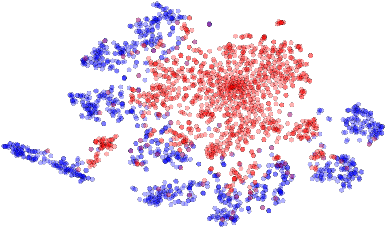
\includegraphics[width=0.45\textwidth]{./figures/adaptation_vis/pool2_mnist2inv_before.pdf}}\hfill%
  \subfigure[Adapted]{%%
    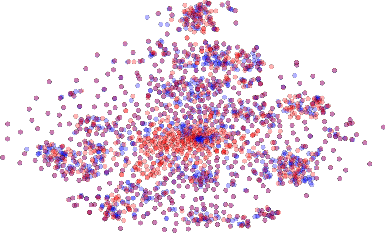
\includegraphics[width=0.45\textwidth]{./figures/adaptation_vis/pool2_mnist2inv_after.pdf}}%%
  \hspace*{\fill}%
  \end{minipage}%
  \begin{minipage}{.5\textwidth}
  \centering
  \small{{\sc Syn Numbers $ \rightarrow $ SVHN}: last hidden layer of the label predictor}
  \setcounter{subfigure}{0}
  \hspace*{\fill}%
  \subfigure[Non-adapted]{%%
    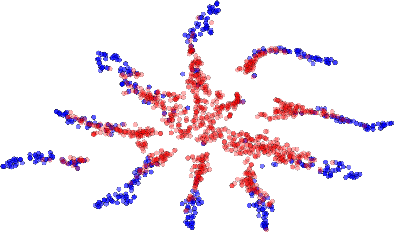
\includegraphics[width=0.45\textwidth]{./figures/adaptation_vis/before.pdf}}\hfill%
  \subfigure[Adapted]{%%
    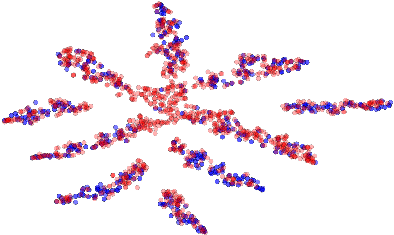
\includegraphics[width=0.45\textwidth]{./figures/adaptation_vis/after.pdf}}%%
  \hspace*{\fill}%
  \end{minipage}
  \caption{The effect of adaptation on the distribution of the extracted features (best viewed in color). The figure shows t-SNE \cite{Maaten13} visualizations of the CNN's activations {\bf (a)} in case when no adaptation was performed and {\bf (b)} in case when our adaptation procedure was incorporated into training. {\it Blue} points correspond to the source domain examples, while {\it red} ones correspond to the target domain. In all cases, the adaptation in our method makes the two distributions of features much closer.}
  \label{fig:exper_adapt_vis}
\end{figure*}

\subsection{Results}
\label{sect:exper_quant}

We now discuss the experimental settings and the results. In each case, we train on the source dataset and test on a different target domain dataset, with considerable shifts between domains (see \fig{exper_domains_examples}). The results are summarized in \tab{results} and \tab{results_office}. 

\vspace{2mm}\noindent {\bf MNIST $ \rightarrow $ MNIST-M.}
Our first experiment deals with the MNIST dataset~\cite{LeCun98} (source). In order to obtain the target domain ({\sc MNIST-M}) we blend digits from the original set over patches randomly extracted from color photos from BSDS500 \cite{Arbelaez11}. This operation is formally defined for two images $ I^{1}, I^{2} $ as $ I_{ijk}^{out} = | I_{ijk}^{1} - I_{ijk}^{2} | $, where $ i, j $ are the coordinates of a pixel and $ k $ is a channel index. In other words, an output sample is produced by taking a patch from a photo and inverting its pixels at positions corresponding to the pixels of a digit. For a human the classification task becomes only slightly harder compared to the original dataset (the digits are still clearly distinguishable) whereas for a CNN trained on MNIST this domain is quite distinct, as the background and the strokes are no longer constant. Consequently, the source-only model performs poorly. Our approach succeeded at aligning feature distributions (\fig{exper_adapt_vis}), which led to successful adaptation results (considering that the adaptation is unsupervised). At the same time, the improvement over source-only model achieved by subspace alignment (SA) \cite{Fernando13} is quite modest, thus highlighting the difficulty of the adaptation task. 

\vspace{2mm}\noindent {\bf Synthetic numbers $ \rightarrow $ SVHN.}
To address a common scenario of training on synthetic data and testing on  real data, we use Street-View House Number dataset {\sc SVHN} \cite{Netzer11} as the target domain and synthetic digits as the source. The latter ({\sc Syn ~Numbers}) consists of ~500,000 images generated by ourselves from Windows fonts by varying the text (that includes different one-, two-, and three-digit numbers), positioning, orientation, background and stroke colors, and the amount of blur. The degrees of variation were chosen manually to simulate SVHN, however the two datasets are still rather distinct, the biggest difference being the structured clutter in the background of SVHN images. 

The proposed backpropagation-based technique works well covering two thirds of the gap between training with source data only and training on target domain data with known target labels. In contrast, SA~\cite{Fernando13} does not result in any significant improvement in the classification accuracy, thus highlighting that the adaptation task is even more challenging than in the case of the MNIST experiment.

\vspace{2mm}\noindent {\bf MNIST $ \leftrightarrow $ SVHN.}
In this experiment, we further increase the gap between distributions, and test on {\sc MNIST} and {\sc SVHN}, which are significantly different in appearance. Training on SVHN even without adaptation is challenging --- classification error stays high during the first 150 epochs. In order to avoid ending up in a poor local minimum we, therefore, do not use learning rate annealing here. Obviously, the two directions ({\sc MNIST} $ \rightarrow $ {\sc SVHN} and {\sc SVHN} $ \rightarrow $ {\sc MNIST}) are not equally difficult. As {\sc SVHN} is more diverse, a model trained on SVHN is expected to be more generic and to perform reasonably on the MNIST dataset. This, indeed, turns out to be the case and is supported by the appearance of the feature distributions. We observe a quite strong separation between the domains when we feed them into the CNN trained solely on { \sc MNIST}, whereas for the {\sc SVHN}-trained network the features are much more intermixed. This difference probably explains why our method succeeded in improving the performance by adaptation in the {\sc SVHN} $ \rightarrow $ {\sc MNIST} scenario (see \tab{results}) but not in the opposite direction (SA is not able to perform adaptation in this case either). Unsupervised adaptation from MNIST to SVHN gives a failure example for our approach (we are unaware of any unsupervised DA methods capable of performing such adaptation).

\vspace{2mm}\noindent {\bf Synthetic Signs $ \rightarrow $ GTSRB.}
Overall, this setting is similar to the {\sc Syn Numbers} $ \rightarrow $ {\sc SVHN} experiment, except the distribution of the features is more complex due to the significantly larger number of classes (43 instead of 10). For the source domain we obtained~100,000 synthetic images (which we call {\sc Syn~Signs}) simulating various photoshooting conditions. Once again, our method achieves a sensible increase in performance once again proving its suitability for the synthetic-to-real data adaptation.

\begin{figure}
  \centering
  \setlength\figureheight{2.7cm}
  \setlength\figurewidth{6.8cm}
  % This file was created by matlab2tikz v0.5.0 running on MATLAB 8.3.
%Copyright (c) 2008--2014, Nico Schlömer <nico.schloemer@gmail.com>
%All rights reserved.
%Minimal pgfplots version: 1.3
%
%The latest updates can be retrieved from
%  http://www.mathworks.com/matlabcentral/fileexchange/22022-matlab2tikz
%where you can also make suggestions and rate matlab2tikz.
%
\begin{tikzpicture}[font=\scriptsize]

\begin{axis}[%
width=0.95092\figurewidth,
height=\figureheight,
at={(0\figurewidth,0\figureheight)},
scale only axis,
xmin=10000,
xmax=50000,
xlabel={Batches seen},
ymin=0,
ymax=1,
ylabel={Validation error},
axis x line*=bottom,
axis y line*=left,
legend style={at={($ (1,1) + (-0.1cm,-0.1cm) $)},anchor=north east,align=left,legend cell align=left,draw=black},
xmajorgrids,
ymajorgrids,
grid style={dashed}
]
\addplot [color=blue,solid,line width=1.0pt]
  table[row sep=crcr]{%
10500	0.199757996632997\\
11000	0.19162984006734\\
11500	0.190788089225589\\
12000	0.192918771043771\\
12500	0.196390993265993\\
13000	0.185527146464646\\
13500	0.190472432659933\\
14000	0.185606060606061\\
14500	0.183422769360269\\
15000	0.189051978114478\\
15500	0.191524621212121\\
16000	0.186079545454545\\
16500	0.179424452861953\\
17000	0.187684132996633\\
17500	0.187868265993266\\
18000	0.180923821548822\\
18500	0.187315867003367\\
19000	0.178661616161616\\
19500	0.18102904040404\\
20000	0.180555555555556\\
20500	0.176662457912458\\
21000	0.183791035353535\\
21500	0.179214015151515\\
22000	0.178898358585859\\
22500	0.178898358585859\\
23000	0.174479166666667\\
23500	0.174742213804714\\
24000	0.171059553872054\\
24500	0.177951388888889\\
25000	0.174794823232323\\
25500	0.174084595959596\\
26000	0.174636994949495\\
26500	0.169034090909091\\
27000	0.171191077441077\\
27500	0.170875420875421\\
28000	0.171506734006734\\
28500	0.170217803030303\\
29000	0.169244528619529\\
29500	0.169875841750842\\
30000	0.168744739057239\\
30500	0.17048085016835\\
31000	0.169454966329966\\
31500	0.167771464646465\\
32000	0.168849957912458\\
32500	0.168323863636364\\
33000	0.168718434343434\\
33500	0.165667087542088\\
34000	0.167376893939394\\
34500	0.169007786195286\\
35000	0.167140151515152\\
35500	0.165667087542088\\
36000	0.167850378787879\\
36500	0.169823232323232\\
37000	0.170691287878788\\
37500	0.16640361952862\\
38000	0.167981902356902\\
38500	0.169875841750842\\
39000	0.166771885521886\\
39500	0.169376052188552\\
40000	0.168087121212121\\
40500	0.165509259259259\\
41000	0.167718855218855\\
41500	0.168060816498317\\
42000	0.166035353535354\\
42500	0.166692971380471\\
43000	0.166429924242424\\
43500	0.167034932659933\\
44000	0.170349326599327\\
44500	0.169744318181818\\
45000	0.168218644781145\\
45500	0.166429924242424\\
46000	0.166324705387205\\
46500	0.168771043771044\\
47000	0.168034511784512\\
47500	0.168718434343434\\
48000	0.171059553872054\\
48500	0.170638678451178\\
49000	0.16819234006734\\
49500	0.168981481481481\\
50000	0.167902988215488\\
};
\addlegendentry{Real data only};

\addplot [color=cyan,solid,line width=1.0pt]
  table[row sep=crcr]{%
10500	0.9625\\
11000	0.79765625\\
11500	0.715625\\
12000	0.6140625\\
12500	0.52109375\\
13000	0.459375\\
13500	0.4484375\\
14000	0.421875\\
14500	0.39453125\\
15000	0.4109375\\
15500	0.34296875\\
16000	0.36875\\
16500	0.3359375\\
17000	0.36171875\\
17500	0.3171875\\
18000	0.3484375\\
18500	0.32421875\\
19000	0.315625\\
19500	0.346875\\
20000	0.31875\\
20500	0.35390625\\
21000	0.3265625\\
21500	0.33359375\\
22000	0.3171875\\
22500	0.28515625\\
23000	0.30546875\\
23500	0.309375\\
24000	0.2796875\\
24500	0.30859375\\
25000	0.30703125\\
25500	0.3078125\\
26000	0.28671875\\
26500	0.2875\\
27000	0.31484375\\
27500	0.2859375\\
28000	0.29375\\
28500	0.31328125\\
29000	0.3078125\\
29500	0.2859375\\
30000	0.2890625\\
30500	0.284375\\
31000	0.2953125\\
31500	0.26953125\\
32000	0.29921875\\
32500	0.30078125\\
33000	0.2640625\\
33500	0.309375\\
34000	0.2734375\\
34500	0.290625\\
35000	0.26796875\\
35500	0.3015625\\
36000	0.26796875\\
36500	0.2921875\\
37000	0.265625\\
37500	0.2765625\\
38000	0.2859375\\
38500	0.32109375\\
39000	0.28046875\\
39500	0.275\\
40000	0.24921875\\
40500	0.29140625\\
41000	0.26640625\\
41500	0.265625\\
42000	0.259375\\
42500	0.2765625\\
43000	0.26796875\\
43500	0.2765625\\
44000	0.27265625\\
44500	0.25546875\\
45000	0.26484375\\
45500	0.271875\\
46000	0.2703125\\
46500	0.26171875\\
47000	0.246875\\
47500	0.25078125\\
48000	0.29609375\\
48500	0.2640625\\
49000	0.26875\\
49500	0.26015625\\
50000	0.2578125\\
};
\addlegendentry{Synthetic data only};

\addplot [color=red,solid,line width=1.0pt]
  table[row sep=crcr]{%
10500	0.943892045454545\\
11000	0.943892045454545\\
11500	0.943892045454545\\
12000	0.943892045454545\\
12500	0.848300715488216\\
13000	0.658722643097643\\
13500	0.590593434343434\\
14000	0.475484006734007\\
14500	0.313946759259259\\
15000	0.235690235690236\\
15500	0.17879313973064\\
16000	0.152383207070707\\
16500	0.12912984006734\\
17000	0.114478114478114\\
17500	0.116214225589226\\
18000	0.1015625\\
18500	0.10066813973064\\
19000	0.101983375420875\\
19500	0.0914351851851852\\
20000	0.0895675505050505\\
20500	0.0894360269360269\\
21000	0.0827283249158249\\
21500	0.0798611111111111\\
22000	0.0859638047138047\\
22500	0.0799137205387205\\
23000	0.0778619528619529\\
23500	0.0737584175084175\\
24000	0.0742582070707071\\
24500	0.0776778198653199\\
25000	0.0771517255892256\\
25500	0.0725747053872054\\
26000	0.0739425505050505\\
26500	0.0734953703703704\\
27000	0.0730744949494949\\
27500	0.0688920454545455\\
28000	0.0702072811447811\\
28500	0.072337962962963\\
29000	0.0670244107744108\\
29500	0.0733638468013468\\
30000	0.0667613636363636\\
30500	0.0692340067340067\\
31000	0.0652093855218855\\
31500	0.0664720117845118\\
32000	0.0655776515151515\\
32500	0.0671296296296296\\
33000	0.0656039562289562\\
33500	0.0646043771043771\\
34000	0.0668665824915825\\
34500	0.0638678451178451\\
35000	0.065077861952862\\
35500	0.0649989478114478\\
36000	0.0672348484848485\\
36500	0.0668665824915825\\
37000	0.0626052188552189\\
37500	0.0652093855218855\\
38000	0.0626315235690236\\
38500	0.0627893518518518\\
39000	0.0613162878787879\\
39500	0.063236531986532\\
40000	0.0629208754208754\\
40500	0.0639467592592593\\
41000	0.0612899831649832\\
41500	0.0653409090909091\\
42000	0.0608691077441077\\
42500	0.0613425925925926\\
43000	0.0630260942760943\\
43500	0.060106271043771\\
44000	0.0638678451178451\\
44500	0.0602377946127946\\
45000	0.0577388468013468\\
45500	0.062684132996633\\
46000	0.0608164983164983\\
46500	0.0603167087542088\\
47000	0.0577651515151515\\
47500	0.0583175505050505\\
48000	0.0591329966329966\\
48500	0.0607112794612795\\
49000	0.0585805976430976\\
49500	0.0583175505050505\\
50000	0.0590540824915825\\
};
\addlegendentry{Both};

\end{axis}
\end{tikzpicture}%
  \caption{Semi-supervised domain adaptation for the traffic signs. As labeled target domain data are shown to the method, it achieves significantly lower error than the model trained on target domain data only or on source domain data only. \vspace{-4mm}}
  \label{fig:exper_semi_test}
\end{figure}

As an additional experiment, we also evaluate the proposed algorithm for semi-supervised domain adaptation, i.e.\ when one is additionally provided with a small amount of labeled target data. For that purpose we split {\sc GTSRB} into the train set (1280 random samples with labels) and the validation set (the rest of the dataset). The validation part is used solely for the evaluation and does not participate in the adaptation. The training procedure changes slightly as the label predictor is now exposed to the target data. \fig{exper_semi_test} shows the change of the validation error throughout the training. While the graph clearly suggests that our method can be used in the semi-supervised setting, thorough verification of semi-supervised setting is left for future work.


\vspace{2mm}\noindent {\bf Office dataset.} 
We finally evaluate our method on {\sc Office} dataset, which is a collection of three distinct domains: {\sc Amazon}, {\sc DSLR}, and {\sc Webcam}. Unlike previously discussed datasets, {\sc Office} is rather small-scale with only 2817 labeled images spread across 31 different categories in the largest domain. The amount of available data is crucial for a successful training of a deep model, hence we opted for the fine-tuning of the CNN pre-trained on the ImageNet \cite{Jia14} as it is done in some recent DA works \cite{Donahue14,Tzeng14,Hoffman14}. We make our approach more comparable with \cite{Tzeng14} by using exactly the same network architecture replacing domain mean-based regularization with the domain classifier.

Following most previous works, we evaluate our method using 5 random splits for each of the 3 transfer tasks commonly used for evaluation. Our training protocol is close to \cite{Tzeng14,Saenko10,Gong12} as we use the same number of labeled source-domain images per category. Unlike those works and similarly to e.g.\ DLID~\cite{Chopra13} we use the whole unlabeled target domain (as the premise of our method is the abundance of unlabeled data in the target domain). Under this transductive setting, our method is able to improve previously-reported state-of-the-art accuracy for unsupervised adaptation very considerably (\tab{results_office}), especially in the most challenging {\sc Amazon} $ \rightarrow $ {\sc Webcam} scenario (the two domains with the largest domain shift).

\section{Conclusion}
\label{conclusions}
The supervised paradigm for training machine reading and comprehension models
provides a promising avenue for making progress on the path to building full
natural language understanding systems. We have demonstrated a methodology for
obtaining a large number of document-query-answer triples and shown that
recurrent and attention based neural networks provide an effective modelling
framework for this task.
Our analysis indicates that the Attentive and Impatient Readers are able to
propagate and integrate semantic information over long distances. In particular
we believe that the incorporation of an attention mechanism is the key
contributor to these results.


The attention mechanism
that we have employed is just one instantiation of a very general idea which
can be further exploited. However, the incorporation of world knowledge and
multi-document queries will also require the development of attention and
embedding mechanisms whose complexity to query does not scale linearly with the
data set size.
There are still many queries requiring complex inference and long range reference resolution that our models are not yet able to answer. As such our data provides a scalable challenge that should support NLP research into the future. Further, significantly bigger training data sets can be acquired using the techniques we have described, undoubtedly allowing us to train more expressive and accurate models.


{\noindent\textbf{Acknowledgments.} We are grateful to ERC StG IDIU-638009 and EPSRC AIMS CDT for support.}
{\small\bibliographystyle{ieee_fullname}\bibliography{main}}
%\clearpage
%%%%%%%%%%%%%%%%%%%%%%%%%%%%%%%%%%%%%%%%%%%%%%%%%%%%%%%%%%%%%%%
%%%%%%%%%%%%%%%%%%%% APPENDIX %%%%%%%%%%%%%%%%%%%%%%%%%%%%%%
%%%%%%%%%%%%%%%%%%%%%%%%%%%%%%%%%%%%%%%%%%%%%%%%%%%%%%%%%%%%%%

\appendix

%\section*{Appendix}

\section{Additional Details on Multi-Scale Processing}
\label{app:detailsMultiscale}

The integration of multi-scale parallel pathways in architectures that use solely unary kernel strides, such as the proposed, was described in Sec.~\ref{subsec:multiscaleCnn}. The required up-sampling of the low-resolution features was performed with simple repetition in our experiments. This was found sufficient, with the following hidden layers learning to combine the multi-scale features. In the case of architectures with strides greater than unary, the last convolutional layers of the two pathways, $L1$ and $L2$, have receptive fields $\boldsymbol{\varphi}_{L1}$ and $\boldsymbol{\varphi}_{L2}$ with strides $\boldsymbol{\tau}_{L1}$ and $\boldsymbol{\tau}_{L2}$ respectively. To preserve spatial correspondence of the multi-scale features and enable the network for dense inference, the dimensions of the input segments should be chosen such that the FMs in $L2$ can be brought to the dimensions of the FMs in $L1$ after sequential resampling by $\uparrow \boldsymbol{\tau}_{L2}$, $\uparrow F_D$, $\downarrow \boldsymbol{\tau}_{L1}$ or equivalent combinations. Here $\uparrow$ and $\downarrow$ represent up- and down-sampling by the given factor. Because they are more reliant on these operations, utilization of more elaborate, learnt upsampling schemes (\cite{Long2014, Ronneberger2015, Noh2015}) should be beneficial in such networks.


\section{Additional Details on Network Configurations}
\label{app:detailsConfig}

\textbf{3D Networks:} The main description of our system is presented in Sec.~\ref{sec:segmentationSystem}. All models discussed in this work outside Sec.~\ref{subsec:val3dContext} are fully 3D CNNs. Their architectures are presented in Table \ref{subtab:netsConfig3d}. They all use the PReLu non-linearity (\cite{he2015delving}). They are trained using the RMSProp optimizer (\cite{rmsProp}) and Nesterov momentum (\cite{sutskever2013importance}) with value $m=0.6$. $L1 = 10^{-6}$ and $L2 = 10^{-4}$ regularisation is applied. We train the networks with dense-training on batches of 10 segments, each of size $25^3$. Exceptions are the experiments in Sec~\ref{subsec:valDenseTraining}, where the batch sizes were adjusted along with the segment sizes, to achieve similar memory footprint and training time per batch. The weights of our shallow, 5-layers networks are initialized by sampling from a normal distribution $\mathcal{N}(0,0.01)$ and their initial learning rate is set to $a=10^{-4}$. Deeper models (and the \quot{Shallow+} model in Sec~\ref{subsec:valDeeper}) use the weight initialisation scheme of \cite{he2015delving}. The scheme increases the signal's variance in our settings, which leads to RMSProm decreasing the effective learning rate. To counter this, we accompany it with an increased initial learning rate $a = 10^{-3}$. Throughout training, the learning rate of all models is halved whenever convergence plateaus. Dropout with 50\% rate is employed on the two last hidden layers of 11-layers deep models.

\textbf{2D Networks:} Table \ref{subtab:netsConfig2d} presents representative examples of 2D configurations that were employed for the experiments discussed in Sec.~\ref{subsec:val3dContext}. Width, depth and batch size were adjusted so that total required memory was similar to the 3D version of DeepMedic. Wider or deeper variants than the ones presented did not show greater performance. A possible reason is that this number of filters is enough for the extraction of the limited 2D information and that the field of view of the deep multi-scale variant is already sufficient for the application. The presented 2D models were regularized with $L1 = 10^{-8}$ and $L2 = 10^{-6}$ since they have less parameters than the 3D variants. All but Dm2dPatch were trained with momentum $m=0.6$ and initial learning rate $a = 10^{-3}$, while the rest with $m=0.9$ and $a = 10^{-2}$ as this setting increased performance. The rest of the hyper parameters are the same as for the 3D DeepMedic.

\setcounter{table}{0}    
\renewcommand\thetable{B.\arabic{table}}

\begin{table}[!h]
\centering
\scriptsize
\caption{Network architectures investigated in Sec.~\ref{sec:vaOfNetArch} and final validation accuracy achieved in the corresponding experiments. (a) 3D and (b) 2D architectures. Columns from left to right: model's name, number of parallel identical pathways and number of feature maps at each of their convolutional layers, number of feature maps at each hidden layer that follows the concatenation of the pathways, dimensions of input segment to the normal and low resolution pathways, batch size and, finally, average DSC achieved on the validation fold. Further configuration details provided in \ref{app:detailsConfig}.}
\label{tab:netsConfig}
\begin{subtable}{1.0\linewidth}
\caption{3D Network Architectures}
\label{subtab:netsConfig3d}
\begin{tabular}{@{}m{1.5cm}m{3.7cm}m{1.2cm}m{1.2cm}m{1.2cm}m{0.8cm}m{1.3cm}}
\toprule	
	               & \#Pathways: FMs/Layer       & FMs/Hidd. & Seg.Norm. & Seg.Low &B.S. & DSC(\%)    \\ \midrule
Shallow(+)         & 1: 30,40,40,50                  & -          & 25x25x25   & -        &10  & 60.2(61.7) \\
Deep(+)            & 1: 30,30,40,40,40,40,50,50      & -          & 25x25x25   & -        &10  & 00.0(64.9)  \\
BigDeep+           & 1: 60,60,80,80,80,80,100,100    & 150,150    & 25x25x25   & -        &10  & 65.2       \\
DeepMedic          & 2: 30,30,40,40,40,40,50,50      & 150,150    & 25x25x25   & 19x19x19 &10  & 66.6       \\ \bottomrule
\end{tabular}
\end{subtable}%
\vspace{10pt}
\begin{subtable}{1.0\linewidth}
\caption{2D Network Architectures}
\label{subtab:netsConfig2d}
\begin{threeparttable}
\begin{tabular}{@{}m{1.5cm}m{3.7cm}m{1.2cm}m{1.2cm}m{1.2cm}m{0.8cm}m{1.3cm}}
\toprule	
	            & \#Pathways: FMs/Layer       & FMs/Hidd. & Seg.Norm. & Seg.Low &B.S. & DSC(\%)    \\ \midrule
%Dm\_3dSeg       & 2: 30,30,40,40,40,40,50,50      & 150,150    & 25x25x17   & 19x19x17   &10 & 62.1       \\
%Dm\_2dPatch 50\% & 2: 30,30,40,40,40,40,50,50      & 150,150    & 17x17x1    & 17x17x1   &540 & 53.7       \\
Dm2dPatch*    	& 2: 30,30,40,40,40,40,50,50      & 150,150    & 17x17x1    & 17x17x1    &540 & 58.8       \\
Dm2dSeg        & 2: 30,30,40,40,40,40,50,50      & 150,150    & 25x25x1    & 19x19x1    &250 & 60.9       \\
Wider2dSeg     & 2: 60,60,80,80,80,80,100,100    & 200,200    & 25x25x1    & 19x19x1    &100 & 61.3       \\
Deeper2dSeg    & 2: 16 layers, linearly 30 to 50 & 150,150    & 41x41x1    & 35x35x1    &100 & 61.5       \\
Large2dSeg  	& 2: 12 layers, linearly 45 to 80 & 200,200    & 33x33x1    & 27x27x1    &100 & 61.3    \\ \bottomrule
\end{tabular}
\begin{tablenotes}
            \item[*] Sampling was manually calibrated to achieve similar class balance as models that are trained on image segments. Model underperformed otherwise.
\end{tablenotes}
\end{threeparttable}
\end{subtable}
\end{table}

\section{Distribution of Tumor Classes Captured in Training}
\label{app:distrTumorClassesTrain}
\setcounter{table}{0}    
\renewcommand\thetable{C.\arabic{table}} 

\hyperref[table:trainingSamplesPercBrats2015Training]{Table C.1}

\begin{table}[!h]
\centering
\scriptsize
\caption{Real distribution of the classes in the training data of BRATS 2015, along with the distribution captured by our proposed training scheme, when segments of size $25^3$ are extracted centred on the tumor and healthy tissue with equal probability. Relative distribution of the foreground classes is closely preserved and the imbalance in comparison to the healthy tissue is automatically alleviated.}
\label{table:trainingSamplesPercBrats2015Training}
\begin{tabular}{@{}lccccc@{}}
\toprule
\multicolumn{1}{c}{} & Healthy		& Necrosis 	& Edema 		& Non-Enh. 	& Enh.Core 	\\ \midrule
Real		 			& 92.42			& 0.43		& 4.87		& 1.02		& 1.27		\\
Captured				& 58.65			& 2.48		& 24.98		& 6.40		& 7.48		\\
\bottomrule
\end{tabular}
\end{table}


%\section{Experiments}
\label{sect:experiments}

% \begin{figure*}
%   \centering
%   \setlength{\tabcolsep}{0pt}
%   \setlength\figurewidth{0.05\textwidth}
%   \newcommand{\example}[1]{\raisebox{-.4\height}{\includegraphics[width=\figurewidth]{./figures/domains_examples/#1}}}
%   \begin{sc}
%   \begin{tabular}{r@{\hskip 1cm} ccccccccccc}
%     MNIST \cite{LeCun98} &
%     \example{mnist_0.png} &
%     \example{mnist_1.png} &
%     \example{mnist_2.png} &
%     \example{mnist_3.png} &
%     \example{mnist_4.png} &
%     \example{mnist_5.png} &
%     \example{mnist_6.png} &
%     \example{mnist_7.png} &
%     \example{mnist_8.png} &
%     \example{mnist_9.png} &
%     \example{mnist_10.png}\\
%     MNIST ($ | \Delta | $, BG) &
%     \example{mnisti_0.png} &
%     \example{mnisti_1.png} &
%     \example{mnisti_2.png} &
%     \example{mnisti_3.png} &
%     \example{mnisti_4.png} &
%     \example{mnisti_5.png} &
%     \example{mnisti_6.png} &
%     \example{mnisti_7.png} &
%     \example{mnisti_8.png} &
%     \example{mnisti_9.png} &
%     \example{mnisti_10.png}\\
%     Syn Numbers &
%     \example{syn_0.png} &
%     \example{syn_1.png} &
%     \example{syn_2.png} &
%     \example{syn_3.png} &
%     \example{syn_4.png} &
%     \example{syn_5.png} &
%     \example{syn_6.png} &
%     \example{syn_7.png} &
%     \example{syn_8.png} &
%     \example{syn_9.png} &
%     \example{syn_10.png}\\
%     SVHN \cite{Netzer11} &
%     \example{svhn_0.png} &
%     \example{svhn_1.png} &
%     \example{svhn_2.png} &
%     \example{svhn_3.png} &
%     \example{svhn_4.png} &
%     \example{svhn_5.png} &
%     \example{svhn_6.png} &
%     \example{svhn_7.png} &
%     \example{svhn_8.png} &
%     \example{svhn_9.png} &
%     \example{svhn_10.png}\\
%     Syn Signs &
%     \example{synsgn_11.png} &
%     \example{synsgn_1.png} &
%     \example{synsgn_2.png} &
%     \example{synsgn_3.png} &
%     \example{synsgn_4.png} &
%     \example{synsgn_5.png} &
%     \example{synsgn_12.png} &
%     \example{synsgn_7.png} &
%     \example{synsgn_8.png} &
%     \example{synsgn_9.png} &
%     \example{synsgn_10.png}\\
%     GTSRB \cite{Stallkamp12} &
%     \example{gtsrb_0.png} &
%     \example{gtsrb_1.png} &
%     \example{gtsrb_2.png} &
%     \example{gtsrb_3.png} &
%     \example{gtsrb_4.png} &
%     \example{gtsrb_5.png} &
%     \example{gtsrb_6.png} &
%     \example{gtsrb_7.png} &
%     \example{gtsrb_8.png} &
%     \example{gtsrb_9.png} &
%     \example{gtsrb_10.png}\\
%     % CIFAR-10 \cite{Krizhevsky09} &
%     % \example{cifar10_0.png} &
%     % \example{cifar10_1.png} &
%     % \example{cifar10_2.png} &
%     % \example{cifar10_3.png} &
%     % \example{cifar10_4.png} &
%     % \example{cifar10_5.png} &
%     % \example{cifar10_11.png} &
%     % \example{cifar10_7.png} &
%     % \example{cifar10_8.png} &
%     % \example{cifar10_9.png} &
%     % \example{cifar10_10.png}\\
%     % STL-10 \cite{Coates11} &
%     % \example{stl10_12.png} &
%     % \example{stl10_1.png} &
%     % \example{stl10_2.png} &
%     % \example{stl10_3.png} &
%     % \example{stl10_4.png} &
%     % \example{stl10_5.png} &
%     % \example{stl10_6.png} &
%     % \example{stl10_13.png} &
%     % \example{stl10_8.png} &
%     % \example{stl10_9.png} &
%     % \example{stl10_10.png}\\
%   \end{tabular}
%   \end{sc}
%   \vskip 2.5mm
%   \caption{\todo[What to do with this figure? Add Office? Remove?]Random samples from the datasets used in the experiments. See \sect{exper_quant} for details.}
%   \label{fig:exper_domains_examples}
% \end{figure*}

\begin{figure*}
  \centering
  \setlength{\tabcolsep}{0pt}
  \setlength\figurewidth{0.05\textwidth}
  \newcommand{\example}[1]{\raisebox{-.4\height}{\includegraphics[width=\figurewidth]{./figures/domains_examples/#1}}}
  \begin{sc}
  \begin{small}
  \begin{tabular}{r@{\hskip 0.5cm} ccc c@{\hskip 0.4cm} ccc c@{\hskip 0.4cm} ccc c@{\hskip 0.4cm} ccc}
    &
    \multicolumn{3}{c}{MNIST} & &
    \multicolumn{3}{c}{Syn Numbers} & &
    \multicolumn{3}{c}{SVHN} & &
    \multicolumn{3}{c}{Syn Signs}\\
    
    Source &
    \example{mnist_0.png} &
    \example{mnist_1.png} &
    \example{mnist_3.png} & &
    
    \example{syn_0.png} &
    \example{syn_1.png} &
    \example{syn_2.png} & &
    
    \example{svhn_3.png} &
    \example{svhn_4.png} &
    \example{svhn_5.png} & &
    
    \example{synsgn_3.png} &
    \example{synsgn_4.png} &
    \example{synsgn_5.png}\\
    
    Target &
    \example{mnisti_0.png} &
    \example{mnisti_1.png} &
    \example{mnisti_2.png} & &
    
    \example{svhn_0.png} &
    \example{svhn_1.png} &
    \example{svhn_2.png} & &
    
    \example{mnist_4.png} &
    \example{mnist_5.png} &
    \example{mnist_6.png} & &
    
    \example{gtsrb_2.png} &
    \example{gtsrb_3.png} &
    \example{gtsrb_4.png}\\
    
    &
    \multicolumn{3}{c}{\rule{0pt}{0.35cm} MNIST-M} & &
    \multicolumn{3}{c}{SVHN} & &
    \multicolumn{3}{c}{MNIST} & &
    \multicolumn{3}{c}{GTSRB}\\
  \end{tabular}
  \end{small}
  \end{sc}
  \caption{Examples of domain pairs used in the experiments. See \sect{exper_quant} for details.}
  \label{fig:exper_domains_examples}
\end{figure*}


\begin{table*}[t]
  \vskip 0.15in
  \begin{center}
    \begin{small}
      \begin{sc}
        \renewcommand{\arraystretch}{1.5}
        \begin{tabular}{l r | c c c c}
          \hline
          \multirow{2}{*}{Method} & {\scriptsize Source} & MNIST & Syn Numbers & SVHN & Syn Signs \\
          & {\scriptsize Target} & MNIST-M & SVHN & MNIST & GTSRB \\
          \hline
          \multicolumn{2}{l |}{Source only} & 
          $ .5749 $                      & $ .8665 $                      & $ .5919 $                      & $ .7400 $                      \\
          \multicolumn{2}{l |}{SA \cite{Fernando13}} & 
          $ .6078 \; (7.9\%) $           & $ .8672 \; (1.3\%) $           & $ .6157 \; (5.9\%) $           & $ .7635 \; (9.1\%) $           \\
          \multicolumn{2}{l |}{Proposed approach} & 
          $ \mathbf{.8149} \; (57.9\%) $ & $ \mathbf{.9048} \; (66.1\%) $ & $ \mathbf{.7107} \; (29.3\%) $ & $ \mathbf{.8866} \; (56.7\%) $ \\
          \multicolumn{2}{l |}{Train on target} & 
          $ .9891 $                      & $ .9244 $                      & $ .9951 $                      & $ .9987 $                      \\
          \hline
        \end{tabular}
      \end{sc}
    \end{small}
  \end{center}
    \caption{Classification accuracies for digit image classifications for different source and target domains. {\sc MNIST-M} corresponds to difference-blended digits over non-uniform background. The first row corresponds to the lower performance bound (i.e.\ if no adaptation is performed). The last row corresponds to training on the target domain data with known class labels (upper bound on the DA performance). For each of the two DA methods (ours and \cite{Fernando13}) we show how much of the gap between the lower and the upper bounds was covered (in brackets). For all five cases, our approach outperforms \cite{Fernando13} considerably, and covers a big portion of the gap.\vspace{-0mm} }
  \label{tab:results}
  \vskip -0.1in
\end{table*}

\begin{table*}[t]
  \vskip 0.15in
  \begin{center}
    \begin{small}
      \begin{sc}
        \renewcommand{\arraystretch}{1.5}
        \begin{tabular}{l r | c c c}
          \hline
          \multirow{2}{*}{Method} & {\scriptsize Source} & Amazon & DSLR & Webcam \\
          & {\scriptsize Target} & Webcam & Webcam & DSLR \\
          \hline
          \multicolumn{2}{l |}{GFK(PLS, PCA) \cite{Gong12}} & 
          $ .464 \pm .005 $ & $ .613 \pm .004 $ & $ .663 \pm .004 $\\ 
          \multicolumn{2}{l |}{SA \cite{Fernando13}} & 
          $ .450 $ & $ .648 $ & $ .699 $\\ 
          \multicolumn{2}{l |}{DA-NBNN \cite{Tommasi13}} & 
          $ .528 \pm .037 $ & $ .766 \pm .017 $ & $ .762 \pm .025 $\\ 
          \multicolumn{2}{l |}{DLID \cite{Chopra13}} & 
          $ .519 $ & $ .782 $ & $ .899 $\\
          \multicolumn{2}{l |}{DeCAF$_6$ Source Only \cite{Donahue14}} &
          $ .522 \pm .017 $ & $ .915 \pm .015 $ & --\\ 
          \multicolumn{2}{l |}{DaNN \cite{Ghifary14}} & 
          $ .536 \pm .002 $ & $ .712 \pm .000 $ & $ .835 \pm .000 $\\ 
          \multicolumn{2}{l |}{DDC \cite{Tzeng14}} & 
          $ .594 \pm .008 $ & $ .925 \pm .003 $ & $ .917 \pm .008 $\\ 
          \multicolumn{2}{l |}{Proposed Approach} & 
          $ \mathbf{ .673 \pm .017 } $ & $ \mathbf{ .940 \pm .008 } $ & $ \mathbf{ .937 \pm .010 } $\\
          \hline
        \end{tabular}
      \end{sc}
    \end{small}
  \end{center}
    \caption{Accuracy evaluation of different DA approaches on the standard {\sc Office} \cite{Saenko10} dataset. Our method (last row) outperforms competitors setting the new state-of-the-art.}
  \label{tab:results_office}
\end{table*}

% Other rows refer to the following algorithms (from top to bottom): Geodesic Flow Kernel \cite{Gong12}, Subspace Alignment \cite{Fernando13}, Naive Bayes Nearest Neighbor \cite{Tommasi13},  deep learning approach from \cite{Chopra13}, DeCAF$_6$-features described in \cite{Donahue14}, Domain Adaptive NNs \cite{Ghifary14}, Deep Domain Confusion \cite{Tzeng14}.

\def\X{{\mathbf X}}
\def\y{{\mathbf y}}

% \vspace{2mm}\noindent {\bf Datasets.}
% \label{sect:exper_datasets}

% In order to test our method in the setting of traffic signs classification we obtained~100,000 synthetic images ({\sc Syn~Signs}) simulating various photoshooting conditions. This dataset was used in conjunction with {\it The German Traffic Sign Recognition Benchmark} ({\sc GTSRB}) \cite{Stallkamp12}.

% Finally, we perform domain adaption for the {\sc CIFAR-10} and the {\sc STL-10} downsampled to the size of $ 32 \times 32 $. This pair is considerably different from the previously mentioned datasets as the intra-class variability here is higher.

We perform extensive evaluation of the proposed approach on a number of popular image datasets and their modifications. These include large-scale datasets of small images popular with deep learning methods, and the {\sc Office} datasets \cite{Saenko10}, which are a {\em de facto} standard for domain adaptation in computer vision, but have much fewer images.

\vspace{2mm}\noindent {\bf Baselines.} For the bulk of experiments the following baselines are evaluated. The \textbf{source-only} model is trained without consideration for target-domain data (no domain classifier branch included into the network). The \textbf{train-on-target} model is trained on the target domain with class labels revealed. This model serves as an upper bound on DA methods, assuming that target data are abundant and the shift between the domains is considerable. 

In addition, we compare our approach against the recently proposed unsupervised DA method based on \textbf{subspace alignment (SA)} \cite{Fernando13}, which is simple to setup and test on new datasets, but has also been shown to perform very well in experimental comparisons with other ``shallow'' DA methods. To boost the performance of this baseline, we pick its most important free parameter (the number of principal components) from the range $ \{ 2, \ldots, 60 \} $, so that the test performance on the target domain is maximized. To apply SA in our setting, we train a source-only model and then consider the activations of the last hidden layer in the label predictor (before the final linear classifier) as descriptors/features, and learn the mapping between the source and the target domains \cite{Fernando13}.

Since the SA baseline requires to train a new classifier after adapting the features, and in order to put all the compared settings on an equal footing, we retrain the last layer of the label predictor using a standard linear SVM~\cite{liblinear} for all four considered methods (including ours; the performance on the target domain remains approximately the same after the retraining). 

For the {\sc Office} dataset \cite{Saenko10}, we directly compare the performance of our full network (feature extractor and label predictor) against recent DA approaches using previously published results.

\vspace{2mm}\noindent {\bf CNN architectures.} In general, we compose feature extractor from two or three convolutional layers, picking their exact configurations from previous works. We give the exact architectures in \ref{sect:appendix_archs}.

For the domain adaptator we stick to the three fully connected layers ($x\rightarrow1024\rightarrow1024\rightarrow2$), except for {\sc MNIST} where we used a simpler ($x\rightarrow100\rightarrow2$) architecture to speed up the experiments.

For loss functions, we set $ L_y $ and $ L_d $ to be the logistic regression loss and the binomial cross-entropy respectively.

\vspace{2mm}\noindent {\bf CNN training procedure.}
The model is trained on $128$-sized batches. Images are preprocessed by the mean subtraction. A half of each batch is populated by the samples from the source domain (with known labels), the rest is comprised of the target domain (with unknown labels).

In order to suppress noisy signal from the domain classifier at the early stages of the training procedure instead of fixing the adaptation factor $ \lambda $, we gradually change it from $0$ to $1$ using the following schedule:
\begin{equation}
  \lambda_p = \frac{2}{1 + \exp(-\gamma \cdot p)} - 1,
\end{equation}
where $\gamma$ was set to $10$ in all experiments (the schedule was not optimized/tweaked). Further details on the CNN training can be found in \ref{sect:appendix_training}.

\vspace{2mm}\noindent {\bf Visualizations.}
We use t-SNE \cite{Maaten13} projection to visualize feature distributions at different points of the network, while color-coding the domains (\fig{exper_adapt_vis}). We observe strong correspondence between the success of the adaptation in terms of the classification accuracy for the target domain, and the overlap between the domain distributions in such visualizations.
 
\vspace{2mm}\noindent {\bf Choosing meta-parameters.} 
In general, good unsupervised DA methods should provide ways to set meta-parameters (such as $\lambda$, the learning rate, the momentum rate, the network architecture for our method) in an unsupervised way, i.e.\ without referring to labeled data in the target domain. %Here we would like to give few recommendations concerning this matter. First, as it was pointed out in \sect{theory} the domain classifier should not be significantly more complex than the label predictor. 
In our method, one can assess the performance of the whole system (and the effect of changing hyper-parameters) by observing the test error on the source domain {\em and} the domain classifier error. In general, we observed a good correspondence between the success of adaptation and these errors (adaptation is more successful when the source domain test error is low, while the domain classifier error is high).
In addition, the layer, where the the domain adaptator is attached can be picked by computing difference between means as suggested in \cite{Tzeng14}. 

% \begin{figure*}
%   \centering
%   {\sc MNIST $ \rightarrow $ MNIST ($ | \Delta | $, bg)}: top feature extractor layer
%   \setcounter{subfigure}{0}
%   \subfigure[Non-adapted]{%%
%     \scalebox{0.8}{%% Creator: Matplotlib, PGF backend
%%
%% To include the figure in your LaTeX document, write
%%   \input{<filename>.pgf}
%%
%% Make sure the required packages are loaded in your preamble
%%   \usepackage{pgf}
%%
%% Figures using additional raster images can only be included by \input if
%% they are in the same directory as the main LaTeX file. For loading figures
%% from other directories you can use the `import` package
%%   \usepackage{import}
%% and then include the figures with
%%   \import{<path to file>}{<filename>.pgf}
%%
%% Matplotlib used the following preamble
%%   \usepackage[utf8x]{inputenc}
%%   \usepackage[T1]{fontenc}
%%
\begingroup%
\makeatletter%
\begin{pgfpicture}%
\pgfpathrectangle{\pgfpointorigin}{\pgfqpoint{3.338520in}{2.040000in}}%
\pgfusepath{use as bounding box}%
\begin{pgfscope}%
\pgfsetbuttcap%
\pgfsetroundjoin%
\definecolor{currentfill}{rgb}{1.000000,1.000000,1.000000}%
\pgfsetfillcolor{currentfill}%
\pgfsetlinewidth{0.000000pt}%
\definecolor{currentstroke}{rgb}{1.000000,1.000000,1.000000}%
\pgfsetstrokecolor{currentstroke}%
\pgfsetdash{}{0pt}%
\pgfpathmoveto{\pgfqpoint{0.000000in}{-0.000000in}}%
\pgfpathlineto{\pgfqpoint{3.338520in}{-0.000000in}}%
\pgfpathlineto{\pgfqpoint{3.338520in}{2.040000in}}%
\pgfpathlineto{\pgfqpoint{0.000000in}{2.040000in}}%
\pgfpathclose%
\pgfusepath{fill}%
\end{pgfscope}%
\begin{pgfscope}%
\pgftext[at=\pgfqpoint{0.510000in}{0.348333in},left,bottom]{\pgfimage[interpolate=true,width=2.553333in,height=1.500000in]{./figures/adaptation_vis/pool2_mnist2inv_before-img0.png}}%
\end{pgfscope}%
\begin{pgfscope}%
\pgftext[at=\pgfqpoint{0.805000in}{0.383333in},left,bottom]{\pgfimage[interpolate=true,width=2.201667in,height=1.371667in]{./figures/adaptation_vis/pool2_mnist2inv_before-img1.png}}%
\end{pgfscope}%
\end{pgfpicture}%
\makeatother%
\endgroup%
}}%%
%   \subfigure[Adapted]{%%
%     \scalebox{0.8}{%% Creator: Matplotlib, PGF backend
%%
%% To include the figure in your LaTeX document, write
%%   \input{<filename>.pgf}
%%
%% Make sure the required packages are loaded in your preamble
%%   \usepackage{pgf}
%%
%% Figures using additional raster images can only be included by \input if
%% they are in the same directory as the main LaTeX file. For loading figures
%% from other directories you can use the `import` package
%%   \usepackage{import}
%% and then include the figures with
%%   \import{<path to file>}{<filename>.pgf}
%%
%% Matplotlib used the following preamble
%%   \usepackage[utf8x]{inputenc}
%%   \usepackage[T1]{fontenc}
%%
\begingroup%
\makeatletter%
\begin{pgfpicture}%
\pgfpathrectangle{\pgfpointorigin}{\pgfqpoint{3.340000in}{2.040000in}}%
\pgfusepath{use as bounding box}%
\begin{pgfscope}%
\pgfsetbuttcap%
\pgfsetroundjoin%
\definecolor{currentfill}{rgb}{1.000000,1.000000,1.000000}%
\pgfsetfillcolor{currentfill}%
\pgfsetlinewidth{0.000000pt}%
\definecolor{currentstroke}{rgb}{1.000000,1.000000,1.000000}%
\pgfsetstrokecolor{currentstroke}%
\pgfsetdash{}{0pt}%
\pgfpathmoveto{\pgfqpoint{0.000000in}{-0.000000in}}%
\pgfpathlineto{\pgfqpoint{3.340000in}{-0.000000in}}%
\pgfpathlineto{\pgfqpoint{3.340000in}{2.040000in}}%
\pgfpathlineto{\pgfqpoint{0.000000in}{2.040000in}}%
\pgfpathclose%
\pgfusepath{fill}%
\end{pgfscope}%
\begin{pgfscope}%
\pgftext[at=\pgfqpoint{0.518333in}{0.321667in},left,bottom]{\pgfimage[interpolate=true,width=2.565000in,height=1.550000in]{./figures/adaptation_vis/pool2_mnist2inv_after-img0.png}}%
\end{pgfscope}%
\begin{pgfscope}%
\pgftext[at=\pgfqpoint{0.518333in}{0.321667in},left,bottom]{\pgfimage[interpolate=true,width=2.565000in,height=1.553333in]{./figures/adaptation_vis/pool2_mnist2inv_after-img1.png}}%
\end{pgfscope}%
\end{pgfpicture}%
\makeatother%
\endgroup%
}}\\
%   \vspace{5mm}
%   {\sc Syn Numbers $ \rightarrow $ SVHN}: last hidden layer of the label predictor
%   \setcounter{subfigure}{0}
%   \subfigure[Non-adapted]{%%
%     \scalebox{0.8}{%% Creator: Matplotlib, PGF backend
%%
%% To include the figure in your LaTeX document, write
%%   \input{<filename>.pgf}
%%
%% Make sure the required packages are loaded in your preamble
%%   \usepackage{pgf}
%%
%% Figures using additional raster images can only be included by \input if
%% they are in the same directory as the main LaTeX file. For loading figures
%% from other directories you can use the `import` package
%%   \usepackage{import}
%% and then include the figures with
%%   \import{<path to file>}{<filename>.pgf}
%%
%% Matplotlib used the following preamble
%%   \usepackage[utf8x]{inputenc}
%%   \usepackage[T1]{fontenc}
%%
\begingroup%
\makeatletter%
\begin{pgfpicture}%
\pgfpathrectangle{\pgfpointorigin}{\pgfqpoint{3.340000in}{2.040000in}}%
\pgfusepath{use as bounding box}%
\begin{pgfscope}%
\pgfsetbuttcap%
\pgfsetroundjoin%
\definecolor{currentfill}{rgb}{1.000000,1.000000,1.000000}%
\pgfsetfillcolor{currentfill}%
\pgfsetlinewidth{0.000000pt}%
\definecolor{currentstroke}{rgb}{1.000000,1.000000,1.000000}%
\pgfsetstrokecolor{currentstroke}%
\pgfsetdash{}{0pt}%
\pgfpathmoveto{\pgfqpoint{0.000000in}{-0.000000in}}%
\pgfpathlineto{\pgfqpoint{3.340000in}{-0.000000in}}%
\pgfpathlineto{\pgfqpoint{3.340000in}{2.040000in}}%
\pgfpathlineto{\pgfqpoint{0.000000in}{2.040000in}}%
\pgfpathclose%
\pgfusepath{fill}%
\end{pgfscope}%
\begin{pgfscope}%
\pgftext[at=\pgfqpoint{0.491667in}{0.335000in},left,bottom]{\pgfimage[interpolate=true,width=2.618333in,height=1.531667in]{./figures/adaptation_vis/before-img0.png}}%
\end{pgfscope}%
\begin{pgfscope}%
\pgftext[at=\pgfqpoint{0.758333in}{0.331667in},left,bottom]{\pgfimage[interpolate=true,width=2.171667in,height=1.436667in]{./figures/adaptation_vis/before-img1.png}}%
\end{pgfscope}%
\begin{pgfscope}%
\pgfsetbuttcap%
\pgfsetroundjoin%
\definecolor{currentfill}{rgb}{0.000000,0.000000,1.000000}%
\pgfsetfillcolor{currentfill}%
\pgfsetfillopacity{0.300000}%
\pgfsetlinewidth{0.150562pt}%
\definecolor{currentstroke}{rgb}{0.000000,0.000000,0.000000}%
\pgfsetstrokecolor{currentstroke}%
\pgfsetstrokeopacity{0.300000}%
\pgfsetdash{}{0pt}%
\pgfpathmoveto{\pgfqpoint{2.521160in}{1.775861in}}%
\pgfpathcurveto{\pgfqpoint{2.525278in}{1.775861in}}{\pgfqpoint{2.529228in}{1.777497in}}{\pgfqpoint{2.532140in}{1.780409in}}%
\pgfpathcurveto{\pgfqpoint{2.535052in}{1.783321in}}{\pgfqpoint{2.536688in}{1.787271in}}{\pgfqpoint{2.536688in}{1.791389in}}%
\pgfpathcurveto{\pgfqpoint{2.536688in}{1.795507in}}{\pgfqpoint{2.535052in}{1.799457in}}{\pgfqpoint{2.532140in}{1.802369in}}%
\pgfpathcurveto{\pgfqpoint{2.529228in}{1.805281in}}{\pgfqpoint{2.525278in}{1.806917in}}{\pgfqpoint{2.521160in}{1.806917in}}%
\pgfpathcurveto{\pgfqpoint{2.517042in}{1.806917in}}{\pgfqpoint{2.513092in}{1.805281in}}{\pgfqpoint{2.510180in}{1.802369in}}%
\pgfpathcurveto{\pgfqpoint{2.507268in}{1.799457in}}{\pgfqpoint{2.505631in}{1.795507in}}{\pgfqpoint{2.505631in}{1.791389in}}%
\pgfpathcurveto{\pgfqpoint{2.505631in}{1.787271in}}{\pgfqpoint{2.507268in}{1.783321in}}{\pgfqpoint{2.510180in}{1.780409in}}%
\pgfpathcurveto{\pgfqpoint{2.513092in}{1.777497in}}{\pgfqpoint{2.517042in}{1.775861in}}{\pgfqpoint{2.521160in}{1.775861in}}%
\pgfpathclose%
\pgfusepath{stroke,fill}%
\end{pgfscope}%
\begin{pgfscope}%
\pgfsetbuttcap%
\pgfsetroundjoin%
\definecolor{currentfill}{rgb}{0.000000,0.000000,1.000000}%
\pgfsetfillcolor{currentfill}%
\pgfsetfillopacity{0.300000}%
\pgfsetlinewidth{0.150562pt}%
\definecolor{currentstroke}{rgb}{0.000000,0.000000,0.000000}%
\pgfsetstrokecolor{currentstroke}%
\pgfsetstrokeopacity{0.300000}%
\pgfsetdash{}{0pt}%
\pgfpathmoveto{\pgfqpoint{2.598938in}{1.785583in}}%
\pgfpathcurveto{\pgfqpoint{2.603056in}{1.785583in}}{\pgfqpoint{2.607006in}{1.787219in}}{\pgfqpoint{2.609918in}{1.790131in}}%
\pgfpathcurveto{\pgfqpoint{2.612830in}{1.793043in}}{\pgfqpoint{2.614466in}{1.796993in}}{\pgfqpoint{2.614466in}{1.801111in}}%
\pgfpathcurveto{\pgfqpoint{2.614466in}{1.805229in}}{\pgfqpoint{2.612830in}{1.809179in}}{\pgfqpoint{2.609918in}{1.812091in}}%
\pgfpathcurveto{\pgfqpoint{2.607006in}{1.815003in}}{\pgfqpoint{2.603056in}{1.816639in}}{\pgfqpoint{2.598938in}{1.816639in}}%
\pgfpathcurveto{\pgfqpoint{2.594819in}{1.816639in}}{\pgfqpoint{2.590869in}{1.815003in}}{\pgfqpoint{2.587957in}{1.812091in}}%
\pgfpathcurveto{\pgfqpoint{2.585045in}{1.809179in}}{\pgfqpoint{2.583409in}{1.805229in}}{\pgfqpoint{2.583409in}{1.801111in}}%
\pgfpathcurveto{\pgfqpoint{2.583409in}{1.796993in}}{\pgfqpoint{2.585045in}{1.793043in}}{\pgfqpoint{2.587957in}{1.790131in}}%
\pgfpathcurveto{\pgfqpoint{2.590869in}{1.787219in}}{\pgfqpoint{2.594819in}{1.785583in}}{\pgfqpoint{2.598938in}{1.785583in}}%
\pgfpathclose%
\pgfusepath{stroke,fill}%
\end{pgfscope}%
\begin{pgfscope}%
\pgfsetbuttcap%
\pgfsetroundjoin%
\definecolor{currentfill}{rgb}{0.000000,0.000000,1.000000}%
\pgfsetfillcolor{currentfill}%
\pgfsetfillopacity{0.300000}%
\pgfsetlinewidth{0.150562pt}%
\definecolor{currentstroke}{rgb}{0.000000,0.000000,0.000000}%
\pgfsetstrokecolor{currentstroke}%
\pgfsetstrokeopacity{0.300000}%
\pgfsetdash{}{0pt}%
\pgfpathmoveto{\pgfqpoint{2.676715in}{1.771000in}}%
\pgfpathcurveto{\pgfqpoint{2.680833in}{1.771000in}}{\pgfqpoint{2.684783in}{1.772636in}}{\pgfqpoint{2.687695in}{1.775548in}}%
\pgfpathcurveto{\pgfqpoint{2.690607in}{1.778460in}}{\pgfqpoint{2.692244in}{1.782410in}}{\pgfqpoint{2.692244in}{1.786528in}}%
\pgfpathcurveto{\pgfqpoint{2.692244in}{1.790646in}}{\pgfqpoint{2.690607in}{1.794596in}}{\pgfqpoint{2.687695in}{1.797508in}}%
\pgfpathcurveto{\pgfqpoint{2.684783in}{1.800420in}}{\pgfqpoint{2.680833in}{1.802056in}}{\pgfqpoint{2.676715in}{1.802056in}}%
\pgfpathcurveto{\pgfqpoint{2.672597in}{1.802056in}}{\pgfqpoint{2.668647in}{1.800420in}}{\pgfqpoint{2.665735in}{1.797508in}}%
\pgfpathcurveto{\pgfqpoint{2.662823in}{1.794596in}}{\pgfqpoint{2.661187in}{1.790646in}}{\pgfqpoint{2.661187in}{1.786528in}}%
\pgfpathcurveto{\pgfqpoint{2.661187in}{1.782410in}}{\pgfqpoint{2.662823in}{1.778460in}}{\pgfqpoint{2.665735in}{1.775548in}}%
\pgfpathcurveto{\pgfqpoint{2.668647in}{1.772636in}}{\pgfqpoint{2.672597in}{1.771000in}}{\pgfqpoint{2.676715in}{1.771000in}}%
\pgfpathclose%
\pgfusepath{stroke,fill}%
\end{pgfscope}%
\begin{pgfscope}%
\pgftext[x=2.798938in,y=1.762222in,left,base]{{\rmfamily\fontsize{8.000000}{9.600000}\selectfont Source}}%
\end{pgfscope}%
\begin{pgfscope}%
\pgfsetbuttcap%
\pgfsetroundjoin%
\definecolor{currentfill}{rgb}{1.000000,0.000000,0.000000}%
\pgfsetfillcolor{currentfill}%
\pgfsetfillopacity{0.300000}%
\pgfsetlinewidth{0.150562pt}%
\definecolor{currentstroke}{rgb}{0.000000,0.000000,0.000000}%
\pgfsetstrokecolor{currentstroke}%
\pgfsetstrokeopacity{0.300000}%
\pgfsetdash{}{0pt}%
\pgfpathmoveto{\pgfqpoint{2.521160in}{1.620928in}}%
\pgfpathcurveto{\pgfqpoint{2.525278in}{1.620928in}}{\pgfqpoint{2.529228in}{1.622564in}}{\pgfqpoint{2.532140in}{1.625476in}}%
\pgfpathcurveto{\pgfqpoint{2.535052in}{1.628388in}}{\pgfqpoint{2.536688in}{1.632338in}}{\pgfqpoint{2.536688in}{1.636456in}}%
\pgfpathcurveto{\pgfqpoint{2.536688in}{1.640574in}}{\pgfqpoint{2.535052in}{1.644524in}}{\pgfqpoint{2.532140in}{1.647436in}}%
\pgfpathcurveto{\pgfqpoint{2.529228in}{1.650348in}}{\pgfqpoint{2.525278in}{1.651984in}}{\pgfqpoint{2.521160in}{1.651984in}}%
\pgfpathcurveto{\pgfqpoint{2.517042in}{1.651984in}}{\pgfqpoint{2.513092in}{1.650348in}}{\pgfqpoint{2.510180in}{1.647436in}}%
\pgfpathcurveto{\pgfqpoint{2.507268in}{1.644524in}}{\pgfqpoint{2.505631in}{1.640574in}}{\pgfqpoint{2.505631in}{1.636456in}}%
\pgfpathcurveto{\pgfqpoint{2.505631in}{1.632338in}}{\pgfqpoint{2.507268in}{1.628388in}}{\pgfqpoint{2.510180in}{1.625476in}}%
\pgfpathcurveto{\pgfqpoint{2.513092in}{1.622564in}}{\pgfqpoint{2.517042in}{1.620928in}}{\pgfqpoint{2.521160in}{1.620928in}}%
\pgfpathclose%
\pgfusepath{stroke,fill}%
\end{pgfscope}%
\begin{pgfscope}%
\pgfsetbuttcap%
\pgfsetroundjoin%
\definecolor{currentfill}{rgb}{1.000000,0.000000,0.000000}%
\pgfsetfillcolor{currentfill}%
\pgfsetfillopacity{0.300000}%
\pgfsetlinewidth{0.150562pt}%
\definecolor{currentstroke}{rgb}{0.000000,0.000000,0.000000}%
\pgfsetstrokecolor{currentstroke}%
\pgfsetstrokeopacity{0.300000}%
\pgfsetdash{}{0pt}%
\pgfpathmoveto{\pgfqpoint{2.598938in}{1.630650in}}%
\pgfpathcurveto{\pgfqpoint{2.603056in}{1.630650in}}{\pgfqpoint{2.607006in}{1.632286in}}{\pgfqpoint{2.609918in}{1.635198in}}%
\pgfpathcurveto{\pgfqpoint{2.612830in}{1.638110in}}{\pgfqpoint{2.614466in}{1.642060in}}{\pgfqpoint{2.614466in}{1.646178in}}%
\pgfpathcurveto{\pgfqpoint{2.614466in}{1.650296in}}{\pgfqpoint{2.612830in}{1.654246in}}{\pgfqpoint{2.609918in}{1.657158in}}%
\pgfpathcurveto{\pgfqpoint{2.607006in}{1.660070in}}{\pgfqpoint{2.603056in}{1.661706in}}{\pgfqpoint{2.598938in}{1.661706in}}%
\pgfpathcurveto{\pgfqpoint{2.594819in}{1.661706in}}{\pgfqpoint{2.590869in}{1.660070in}}{\pgfqpoint{2.587957in}{1.657158in}}%
\pgfpathcurveto{\pgfqpoint{2.585045in}{1.654246in}}{\pgfqpoint{2.583409in}{1.650296in}}{\pgfqpoint{2.583409in}{1.646178in}}%
\pgfpathcurveto{\pgfqpoint{2.583409in}{1.642060in}}{\pgfqpoint{2.585045in}{1.638110in}}{\pgfqpoint{2.587957in}{1.635198in}}%
\pgfpathcurveto{\pgfqpoint{2.590869in}{1.632286in}}{\pgfqpoint{2.594819in}{1.630650in}}{\pgfqpoint{2.598938in}{1.630650in}}%
\pgfpathclose%
\pgfusepath{stroke,fill}%
\end{pgfscope}%
\begin{pgfscope}%
\pgfsetbuttcap%
\pgfsetroundjoin%
\definecolor{currentfill}{rgb}{1.000000,0.000000,0.000000}%
\pgfsetfillcolor{currentfill}%
\pgfsetfillopacity{0.300000}%
\pgfsetlinewidth{0.150562pt}%
\definecolor{currentstroke}{rgb}{0.000000,0.000000,0.000000}%
\pgfsetstrokecolor{currentstroke}%
\pgfsetstrokeopacity{0.300000}%
\pgfsetdash{}{0pt}%
\pgfpathmoveto{\pgfqpoint{2.676715in}{1.616066in}}%
\pgfpathcurveto{\pgfqpoint{2.680833in}{1.616066in}}{\pgfqpoint{2.684783in}{1.617703in}}{\pgfqpoint{2.687695in}{1.620615in}}%
\pgfpathcurveto{\pgfqpoint{2.690607in}{1.623527in}}{\pgfqpoint{2.692244in}{1.627477in}}{\pgfqpoint{2.692244in}{1.631595in}}%
\pgfpathcurveto{\pgfqpoint{2.692244in}{1.635713in}}{\pgfqpoint{2.690607in}{1.639663in}}{\pgfqpoint{2.687695in}{1.642575in}}%
\pgfpathcurveto{\pgfqpoint{2.684783in}{1.645487in}}{\pgfqpoint{2.680833in}{1.647123in}}{\pgfqpoint{2.676715in}{1.647123in}}%
\pgfpathcurveto{\pgfqpoint{2.672597in}{1.647123in}}{\pgfqpoint{2.668647in}{1.645487in}}{\pgfqpoint{2.665735in}{1.642575in}}%
\pgfpathcurveto{\pgfqpoint{2.662823in}{1.639663in}}{\pgfqpoint{2.661187in}{1.635713in}}{\pgfqpoint{2.661187in}{1.631595in}}%
\pgfpathcurveto{\pgfqpoint{2.661187in}{1.627477in}}{\pgfqpoint{2.662823in}{1.623527in}}{\pgfqpoint{2.665735in}{1.620615in}}%
\pgfpathcurveto{\pgfqpoint{2.668647in}{1.617703in}}{\pgfqpoint{2.672597in}{1.616066in}}{\pgfqpoint{2.676715in}{1.616066in}}%
\pgfpathclose%
\pgfusepath{stroke,fill}%
\end{pgfscope}%
\begin{pgfscope}%
\pgftext[x=2.798938in,y=1.607289in,left,base]{{\rmfamily\fontsize{8.000000}{9.600000}\selectfont Target}}%
\end{pgfscope}%
\end{pgfpicture}%
\makeatother%
\endgroup%
}}%%
%   \subfigure[Adapted]{%%
%     \scalebox{0.8}{%% Creator: Matplotlib, PGF backend
%%
%% To include the figure in your LaTeX document, write
%%   \input{<filename>.pgf}
%%
%% Make sure the required packages are loaded in your preamble
%%   \usepackage{pgf}
%%
%% Figures using additional raster images can only be included by \input if
%% they are in the same directory as the main LaTeX file. For loading figures
%% from other directories you can use the `import` package
%%   \usepackage{import}
%% and then include the figures with
%%   \import{<path to file>}{<filename>.pgf}
%%
%% Matplotlib used the following preamble
%%   \usepackage[utf8x]{inputenc}
%%   \usepackage[T1]{fontenc}
%%
\begingroup%
\makeatletter%
\begin{pgfpicture}%
\pgfpathrectangle{\pgfpointorigin}{\pgfqpoint{3.340000in}{2.040000in}}%
\pgfusepath{use as bounding box}%
\begin{pgfscope}%
\pgfsetbuttcap%
\pgfsetroundjoin%
\definecolor{currentfill}{rgb}{1.000000,1.000000,1.000000}%
\pgfsetfillcolor{currentfill}%
\pgfsetlinewidth{0.000000pt}%
\definecolor{currentstroke}{rgb}{1.000000,1.000000,1.000000}%
\pgfsetstrokecolor{currentstroke}%
\pgfsetdash{}{0pt}%
\pgfpathmoveto{\pgfqpoint{0.000000in}{-0.000000in}}%
\pgfpathlineto{\pgfqpoint{3.340000in}{-0.000000in}}%
\pgfpathlineto{\pgfqpoint{3.340000in}{2.040000in}}%
\pgfpathlineto{\pgfqpoint{0.000000in}{2.040000in}}%
\pgfpathclose%
\pgfusepath{fill}%
\end{pgfscope}%
\begin{pgfscope}%
\pgftext[at=\pgfqpoint{0.501667in}{0.330000in},left,bottom]{\pgfimage[interpolate=true,width=2.600000in,height=1.540000in]{./figures/adaptation_vis/after-img0.png}}%
\end{pgfscope}%
\begin{pgfscope}%
\pgftext[at=\pgfqpoint{0.500000in}{0.320000in},left,bottom]{\pgfimage[interpolate=true,width=2.585000in,height=1.556667in]{./figures/adaptation_vis/after-img1.png}}%
\end{pgfscope}%
\begin{pgfscope}%
\pgfsetbuttcap%
\pgfsetroundjoin%
\definecolor{currentfill}{rgb}{0.000000,0.000000,1.000000}%
\pgfsetfillcolor{currentfill}%
\pgfsetfillopacity{0.300000}%
\pgfsetlinewidth{0.150562pt}%
\definecolor{currentstroke}{rgb}{0.000000,0.000000,0.000000}%
\pgfsetstrokecolor{currentstroke}%
\pgfsetstrokeopacity{0.300000}%
\pgfsetdash{}{0pt}%
\pgfpathmoveto{\pgfqpoint{2.521160in}{1.775861in}}%
\pgfpathcurveto{\pgfqpoint{2.525278in}{1.775861in}}{\pgfqpoint{2.529228in}{1.777497in}}{\pgfqpoint{2.532140in}{1.780409in}}%
\pgfpathcurveto{\pgfqpoint{2.535052in}{1.783321in}}{\pgfqpoint{2.536688in}{1.787271in}}{\pgfqpoint{2.536688in}{1.791389in}}%
\pgfpathcurveto{\pgfqpoint{2.536688in}{1.795507in}}{\pgfqpoint{2.535052in}{1.799457in}}{\pgfqpoint{2.532140in}{1.802369in}}%
\pgfpathcurveto{\pgfqpoint{2.529228in}{1.805281in}}{\pgfqpoint{2.525278in}{1.806917in}}{\pgfqpoint{2.521160in}{1.806917in}}%
\pgfpathcurveto{\pgfqpoint{2.517042in}{1.806917in}}{\pgfqpoint{2.513092in}{1.805281in}}{\pgfqpoint{2.510180in}{1.802369in}}%
\pgfpathcurveto{\pgfqpoint{2.507268in}{1.799457in}}{\pgfqpoint{2.505631in}{1.795507in}}{\pgfqpoint{2.505631in}{1.791389in}}%
\pgfpathcurveto{\pgfqpoint{2.505631in}{1.787271in}}{\pgfqpoint{2.507268in}{1.783321in}}{\pgfqpoint{2.510180in}{1.780409in}}%
\pgfpathcurveto{\pgfqpoint{2.513092in}{1.777497in}}{\pgfqpoint{2.517042in}{1.775861in}}{\pgfqpoint{2.521160in}{1.775861in}}%
\pgfpathclose%
\pgfusepath{stroke,fill}%
\end{pgfscope}%
\begin{pgfscope}%
\pgfsetbuttcap%
\pgfsetroundjoin%
\definecolor{currentfill}{rgb}{0.000000,0.000000,1.000000}%
\pgfsetfillcolor{currentfill}%
\pgfsetfillopacity{0.300000}%
\pgfsetlinewidth{0.150562pt}%
\definecolor{currentstroke}{rgb}{0.000000,0.000000,0.000000}%
\pgfsetstrokecolor{currentstroke}%
\pgfsetstrokeopacity{0.300000}%
\pgfsetdash{}{0pt}%
\pgfpathmoveto{\pgfqpoint{2.598938in}{1.785583in}}%
\pgfpathcurveto{\pgfqpoint{2.603056in}{1.785583in}}{\pgfqpoint{2.607006in}{1.787219in}}{\pgfqpoint{2.609918in}{1.790131in}}%
\pgfpathcurveto{\pgfqpoint{2.612830in}{1.793043in}}{\pgfqpoint{2.614466in}{1.796993in}}{\pgfqpoint{2.614466in}{1.801111in}}%
\pgfpathcurveto{\pgfqpoint{2.614466in}{1.805229in}}{\pgfqpoint{2.612830in}{1.809179in}}{\pgfqpoint{2.609918in}{1.812091in}}%
\pgfpathcurveto{\pgfqpoint{2.607006in}{1.815003in}}{\pgfqpoint{2.603056in}{1.816639in}}{\pgfqpoint{2.598938in}{1.816639in}}%
\pgfpathcurveto{\pgfqpoint{2.594819in}{1.816639in}}{\pgfqpoint{2.590869in}{1.815003in}}{\pgfqpoint{2.587957in}{1.812091in}}%
\pgfpathcurveto{\pgfqpoint{2.585045in}{1.809179in}}{\pgfqpoint{2.583409in}{1.805229in}}{\pgfqpoint{2.583409in}{1.801111in}}%
\pgfpathcurveto{\pgfqpoint{2.583409in}{1.796993in}}{\pgfqpoint{2.585045in}{1.793043in}}{\pgfqpoint{2.587957in}{1.790131in}}%
\pgfpathcurveto{\pgfqpoint{2.590869in}{1.787219in}}{\pgfqpoint{2.594819in}{1.785583in}}{\pgfqpoint{2.598938in}{1.785583in}}%
\pgfpathclose%
\pgfusepath{stroke,fill}%
\end{pgfscope}%
\begin{pgfscope}%
\pgfsetbuttcap%
\pgfsetroundjoin%
\definecolor{currentfill}{rgb}{0.000000,0.000000,1.000000}%
\pgfsetfillcolor{currentfill}%
\pgfsetfillopacity{0.300000}%
\pgfsetlinewidth{0.150562pt}%
\definecolor{currentstroke}{rgb}{0.000000,0.000000,0.000000}%
\pgfsetstrokecolor{currentstroke}%
\pgfsetstrokeopacity{0.300000}%
\pgfsetdash{}{0pt}%
\pgfpathmoveto{\pgfqpoint{2.676715in}{1.771000in}}%
\pgfpathcurveto{\pgfqpoint{2.680833in}{1.771000in}}{\pgfqpoint{2.684783in}{1.772636in}}{\pgfqpoint{2.687695in}{1.775548in}}%
\pgfpathcurveto{\pgfqpoint{2.690607in}{1.778460in}}{\pgfqpoint{2.692244in}{1.782410in}}{\pgfqpoint{2.692244in}{1.786528in}}%
\pgfpathcurveto{\pgfqpoint{2.692244in}{1.790646in}}{\pgfqpoint{2.690607in}{1.794596in}}{\pgfqpoint{2.687695in}{1.797508in}}%
\pgfpathcurveto{\pgfqpoint{2.684783in}{1.800420in}}{\pgfqpoint{2.680833in}{1.802056in}}{\pgfqpoint{2.676715in}{1.802056in}}%
\pgfpathcurveto{\pgfqpoint{2.672597in}{1.802056in}}{\pgfqpoint{2.668647in}{1.800420in}}{\pgfqpoint{2.665735in}{1.797508in}}%
\pgfpathcurveto{\pgfqpoint{2.662823in}{1.794596in}}{\pgfqpoint{2.661187in}{1.790646in}}{\pgfqpoint{2.661187in}{1.786528in}}%
\pgfpathcurveto{\pgfqpoint{2.661187in}{1.782410in}}{\pgfqpoint{2.662823in}{1.778460in}}{\pgfqpoint{2.665735in}{1.775548in}}%
\pgfpathcurveto{\pgfqpoint{2.668647in}{1.772636in}}{\pgfqpoint{2.672597in}{1.771000in}}{\pgfqpoint{2.676715in}{1.771000in}}%
\pgfpathclose%
\pgfusepath{stroke,fill}%
\end{pgfscope}%
\begin{pgfscope}%
\pgftext[x=2.798938in,y=1.762222in,left,base]{{\rmfamily\fontsize{8.000000}{9.600000}\selectfont Source}}%
\end{pgfscope}%
\begin{pgfscope}%
\pgfsetbuttcap%
\pgfsetroundjoin%
\definecolor{currentfill}{rgb}{1.000000,0.000000,0.000000}%
\pgfsetfillcolor{currentfill}%
\pgfsetfillopacity{0.300000}%
\pgfsetlinewidth{0.150562pt}%
\definecolor{currentstroke}{rgb}{0.000000,0.000000,0.000000}%
\pgfsetstrokecolor{currentstroke}%
\pgfsetstrokeopacity{0.300000}%
\pgfsetdash{}{0pt}%
\pgfpathmoveto{\pgfqpoint{2.521160in}{1.620928in}}%
\pgfpathcurveto{\pgfqpoint{2.525278in}{1.620928in}}{\pgfqpoint{2.529228in}{1.622564in}}{\pgfqpoint{2.532140in}{1.625476in}}%
\pgfpathcurveto{\pgfqpoint{2.535052in}{1.628388in}}{\pgfqpoint{2.536688in}{1.632338in}}{\pgfqpoint{2.536688in}{1.636456in}}%
\pgfpathcurveto{\pgfqpoint{2.536688in}{1.640574in}}{\pgfqpoint{2.535052in}{1.644524in}}{\pgfqpoint{2.532140in}{1.647436in}}%
\pgfpathcurveto{\pgfqpoint{2.529228in}{1.650348in}}{\pgfqpoint{2.525278in}{1.651984in}}{\pgfqpoint{2.521160in}{1.651984in}}%
\pgfpathcurveto{\pgfqpoint{2.517042in}{1.651984in}}{\pgfqpoint{2.513092in}{1.650348in}}{\pgfqpoint{2.510180in}{1.647436in}}%
\pgfpathcurveto{\pgfqpoint{2.507268in}{1.644524in}}{\pgfqpoint{2.505631in}{1.640574in}}{\pgfqpoint{2.505631in}{1.636456in}}%
\pgfpathcurveto{\pgfqpoint{2.505631in}{1.632338in}}{\pgfqpoint{2.507268in}{1.628388in}}{\pgfqpoint{2.510180in}{1.625476in}}%
\pgfpathcurveto{\pgfqpoint{2.513092in}{1.622564in}}{\pgfqpoint{2.517042in}{1.620928in}}{\pgfqpoint{2.521160in}{1.620928in}}%
\pgfpathclose%
\pgfusepath{stroke,fill}%
\end{pgfscope}%
\begin{pgfscope}%
\pgfsetbuttcap%
\pgfsetroundjoin%
\definecolor{currentfill}{rgb}{1.000000,0.000000,0.000000}%
\pgfsetfillcolor{currentfill}%
\pgfsetfillopacity{0.300000}%
\pgfsetlinewidth{0.150562pt}%
\definecolor{currentstroke}{rgb}{0.000000,0.000000,0.000000}%
\pgfsetstrokecolor{currentstroke}%
\pgfsetstrokeopacity{0.300000}%
\pgfsetdash{}{0pt}%
\pgfpathmoveto{\pgfqpoint{2.598938in}{1.630650in}}%
\pgfpathcurveto{\pgfqpoint{2.603056in}{1.630650in}}{\pgfqpoint{2.607006in}{1.632286in}}{\pgfqpoint{2.609918in}{1.635198in}}%
\pgfpathcurveto{\pgfqpoint{2.612830in}{1.638110in}}{\pgfqpoint{2.614466in}{1.642060in}}{\pgfqpoint{2.614466in}{1.646178in}}%
\pgfpathcurveto{\pgfqpoint{2.614466in}{1.650296in}}{\pgfqpoint{2.612830in}{1.654246in}}{\pgfqpoint{2.609918in}{1.657158in}}%
\pgfpathcurveto{\pgfqpoint{2.607006in}{1.660070in}}{\pgfqpoint{2.603056in}{1.661706in}}{\pgfqpoint{2.598938in}{1.661706in}}%
\pgfpathcurveto{\pgfqpoint{2.594819in}{1.661706in}}{\pgfqpoint{2.590869in}{1.660070in}}{\pgfqpoint{2.587957in}{1.657158in}}%
\pgfpathcurveto{\pgfqpoint{2.585045in}{1.654246in}}{\pgfqpoint{2.583409in}{1.650296in}}{\pgfqpoint{2.583409in}{1.646178in}}%
\pgfpathcurveto{\pgfqpoint{2.583409in}{1.642060in}}{\pgfqpoint{2.585045in}{1.638110in}}{\pgfqpoint{2.587957in}{1.635198in}}%
\pgfpathcurveto{\pgfqpoint{2.590869in}{1.632286in}}{\pgfqpoint{2.594819in}{1.630650in}}{\pgfqpoint{2.598938in}{1.630650in}}%
\pgfpathclose%
\pgfusepath{stroke,fill}%
\end{pgfscope}%
\begin{pgfscope}%
\pgfsetbuttcap%
\pgfsetroundjoin%
\definecolor{currentfill}{rgb}{1.000000,0.000000,0.000000}%
\pgfsetfillcolor{currentfill}%
\pgfsetfillopacity{0.300000}%
\pgfsetlinewidth{0.150562pt}%
\definecolor{currentstroke}{rgb}{0.000000,0.000000,0.000000}%
\pgfsetstrokecolor{currentstroke}%
\pgfsetstrokeopacity{0.300000}%
\pgfsetdash{}{0pt}%
\pgfpathmoveto{\pgfqpoint{2.676715in}{1.616066in}}%
\pgfpathcurveto{\pgfqpoint{2.680833in}{1.616066in}}{\pgfqpoint{2.684783in}{1.617703in}}{\pgfqpoint{2.687695in}{1.620615in}}%
\pgfpathcurveto{\pgfqpoint{2.690607in}{1.623527in}}{\pgfqpoint{2.692244in}{1.627477in}}{\pgfqpoint{2.692244in}{1.631595in}}%
\pgfpathcurveto{\pgfqpoint{2.692244in}{1.635713in}}{\pgfqpoint{2.690607in}{1.639663in}}{\pgfqpoint{2.687695in}{1.642575in}}%
\pgfpathcurveto{\pgfqpoint{2.684783in}{1.645487in}}{\pgfqpoint{2.680833in}{1.647123in}}{\pgfqpoint{2.676715in}{1.647123in}}%
\pgfpathcurveto{\pgfqpoint{2.672597in}{1.647123in}}{\pgfqpoint{2.668647in}{1.645487in}}{\pgfqpoint{2.665735in}{1.642575in}}%
\pgfpathcurveto{\pgfqpoint{2.662823in}{1.639663in}}{\pgfqpoint{2.661187in}{1.635713in}}{\pgfqpoint{2.661187in}{1.631595in}}%
\pgfpathcurveto{\pgfqpoint{2.661187in}{1.627477in}}{\pgfqpoint{2.662823in}{1.623527in}}{\pgfqpoint{2.665735in}{1.620615in}}%
\pgfpathcurveto{\pgfqpoint{2.668647in}{1.617703in}}{\pgfqpoint{2.672597in}{1.616066in}}{\pgfqpoint{2.676715in}{1.616066in}}%
\pgfpathclose%
\pgfusepath{stroke,fill}%
\end{pgfscope}%
\begin{pgfscope}%
\pgftext[x=2.798938in,y=1.607289in,left,base]{{\rmfamily\fontsize{8.000000}{9.600000}\selectfont Target}}%
\end{pgfscope}%
\end{pgfpicture}%
\makeatother%
\endgroup%
}}%%
%   \caption{The effect of adaptation on the distribution of the extracted features. The figure shows t-SNE \cite{Maaten13} visualizations of the CNN's activations {\bf (a)} in case when no adaptation was performed and {\bf (b)} in case when our adaptation procedure was incorporated into training. {\it Blue} points correspond to the source domain examples, while {\it red} ones correspond to the target domain. In all cases, the adaptation in our method makes the two distributions of features much closer.}
%   \label{fig:exper_adapt_vis}
% \end{figure*}

\begin{figure*}
  \addtolength{\subfigcapskip}{0.1cm}
  \centering
  \begin{minipage}{.5\textwidth}
  \centering
  \small{{\sc MNIST $ \rightarrow $ MNIST-M}: top feature extractor layer}
  \setcounter{subfigure}{0}
  \hspace*{\fill}%
  \subfigure[Non-adapted]{%%
    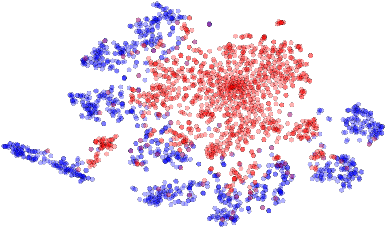
\includegraphics[width=0.45\textwidth]{./figures/adaptation_vis/pool2_mnist2inv_before.pdf}}\hfill%
  \subfigure[Adapted]{%%
    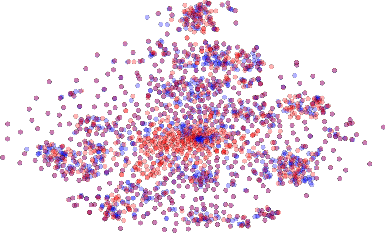
\includegraphics[width=0.45\textwidth]{./figures/adaptation_vis/pool2_mnist2inv_after.pdf}}%%
  \hspace*{\fill}%
  \end{minipage}%
  \begin{minipage}{.5\textwidth}
  \centering
  \small{{\sc Syn Numbers $ \rightarrow $ SVHN}: last hidden layer of the label predictor}
  \setcounter{subfigure}{0}
  \hspace*{\fill}%
  \subfigure[Non-adapted]{%%
    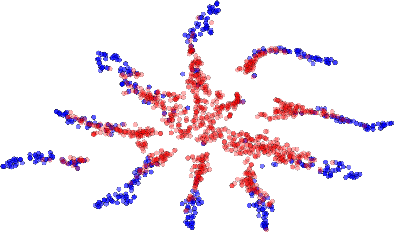
\includegraphics[width=0.45\textwidth]{./figures/adaptation_vis/before.pdf}}\hfill%
  \subfigure[Adapted]{%%
    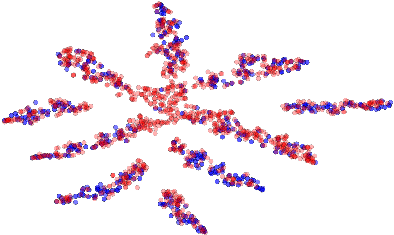
\includegraphics[width=0.45\textwidth]{./figures/adaptation_vis/after.pdf}}%%
  \hspace*{\fill}%
  \end{minipage}
  \caption{The effect of adaptation on the distribution of the extracted features (best viewed in color). The figure shows t-SNE \cite{Maaten13} visualizations of the CNN's activations {\bf (a)} in case when no adaptation was performed and {\bf (b)} in case when our adaptation procedure was incorporated into training. {\it Blue} points correspond to the source domain examples, while {\it red} ones correspond to the target domain. In all cases, the adaptation in our method makes the two distributions of features much closer.}
  \label{fig:exper_adapt_vis}
\end{figure*}

\subsection{Results}
\label{sect:exper_quant}

We now discuss the experimental settings and the results. In each case, we train on the source dataset and test on a different target domain dataset, with considerable shifts between domains (see \fig{exper_domains_examples}). The results are summarized in \tab{results} and \tab{results_office}. 

\vspace{2mm}\noindent {\bf MNIST $ \rightarrow $ MNIST-M.}
Our first experiment deals with the MNIST dataset~\cite{LeCun98} (source). In order to obtain the target domain ({\sc MNIST-M}) we blend digits from the original set over patches randomly extracted from color photos from BSDS500 \cite{Arbelaez11}. This operation is formally defined for two images $ I^{1}, I^{2} $ as $ I_{ijk}^{out} = | I_{ijk}^{1} - I_{ijk}^{2} | $, where $ i, j $ are the coordinates of a pixel and $ k $ is a channel index. In other words, an output sample is produced by taking a patch from a photo and inverting its pixels at positions corresponding to the pixels of a digit. For a human the classification task becomes only slightly harder compared to the original dataset (the digits are still clearly distinguishable) whereas for a CNN trained on MNIST this domain is quite distinct, as the background and the strokes are no longer constant. Consequently, the source-only model performs poorly. Our approach succeeded at aligning feature distributions (\fig{exper_adapt_vis}), which led to successful adaptation results (considering that the adaptation is unsupervised). At the same time, the improvement over source-only model achieved by subspace alignment (SA) \cite{Fernando13} is quite modest, thus highlighting the difficulty of the adaptation task. 

\vspace{2mm}\noindent {\bf Synthetic numbers $ \rightarrow $ SVHN.}
To address a common scenario of training on synthetic data and testing on  real data, we use Street-View House Number dataset {\sc SVHN} \cite{Netzer11} as the target domain and synthetic digits as the source. The latter ({\sc Syn ~Numbers}) consists of ~500,000 images generated by ourselves from Windows fonts by varying the text (that includes different one-, two-, and three-digit numbers), positioning, orientation, background and stroke colors, and the amount of blur. The degrees of variation were chosen manually to simulate SVHN, however the two datasets are still rather distinct, the biggest difference being the structured clutter in the background of SVHN images. 

The proposed backpropagation-based technique works well covering two thirds of the gap between training with source data only and training on target domain data with known target labels. In contrast, SA~\cite{Fernando13} does not result in any significant improvement in the classification accuracy, thus highlighting that the adaptation task is even more challenging than in the case of the MNIST experiment.

\vspace{2mm}\noindent {\bf MNIST $ \leftrightarrow $ SVHN.}
In this experiment, we further increase the gap between distributions, and test on {\sc MNIST} and {\sc SVHN}, which are significantly different in appearance. Training on SVHN even without adaptation is challenging --- classification error stays high during the first 150 epochs. In order to avoid ending up in a poor local minimum we, therefore, do not use learning rate annealing here. Obviously, the two directions ({\sc MNIST} $ \rightarrow $ {\sc SVHN} and {\sc SVHN} $ \rightarrow $ {\sc MNIST}) are not equally difficult. As {\sc SVHN} is more diverse, a model trained on SVHN is expected to be more generic and to perform reasonably on the MNIST dataset. This, indeed, turns out to be the case and is supported by the appearance of the feature distributions. We observe a quite strong separation between the domains when we feed them into the CNN trained solely on { \sc MNIST}, whereas for the {\sc SVHN}-trained network the features are much more intermixed. This difference probably explains why our method succeeded in improving the performance by adaptation in the {\sc SVHN} $ \rightarrow $ {\sc MNIST} scenario (see \tab{results}) but not in the opposite direction (SA is not able to perform adaptation in this case either). Unsupervised adaptation from MNIST to SVHN gives a failure example for our approach (we are unaware of any unsupervised DA methods capable of performing such adaptation).

\vspace{2mm}\noindent {\bf Synthetic Signs $ \rightarrow $ GTSRB.}
Overall, this setting is similar to the {\sc Syn Numbers} $ \rightarrow $ {\sc SVHN} experiment, except the distribution of the features is more complex due to the significantly larger number of classes (43 instead of 10). For the source domain we obtained~100,000 synthetic images (which we call {\sc Syn~Signs}) simulating various photoshooting conditions. Once again, our method achieves a sensible increase in performance once again proving its suitability for the synthetic-to-real data adaptation.

\begin{figure}
  \centering
  \setlength\figureheight{2.7cm}
  \setlength\figurewidth{6.8cm}
  % This file was created by matlab2tikz v0.5.0 running on MATLAB 8.3.
%Copyright (c) 2008--2014, Nico Schlömer <nico.schloemer@gmail.com>
%All rights reserved.
%Minimal pgfplots version: 1.3
%
%The latest updates can be retrieved from
%  http://www.mathworks.com/matlabcentral/fileexchange/22022-matlab2tikz
%where you can also make suggestions and rate matlab2tikz.
%
\begin{tikzpicture}[font=\scriptsize]

\begin{axis}[%
width=0.95092\figurewidth,
height=\figureheight,
at={(0\figurewidth,0\figureheight)},
scale only axis,
xmin=10000,
xmax=50000,
xlabel={Batches seen},
ymin=0,
ymax=1,
ylabel={Validation error},
axis x line*=bottom,
axis y line*=left,
legend style={at={($ (1,1) + (-0.1cm,-0.1cm) $)},anchor=north east,align=left,legend cell align=left,draw=black},
xmajorgrids,
ymajorgrids,
grid style={dashed}
]
\addplot [color=blue,solid,line width=1.0pt]
  table[row sep=crcr]{%
10500	0.199757996632997\\
11000	0.19162984006734\\
11500	0.190788089225589\\
12000	0.192918771043771\\
12500	0.196390993265993\\
13000	0.185527146464646\\
13500	0.190472432659933\\
14000	0.185606060606061\\
14500	0.183422769360269\\
15000	0.189051978114478\\
15500	0.191524621212121\\
16000	0.186079545454545\\
16500	0.179424452861953\\
17000	0.187684132996633\\
17500	0.187868265993266\\
18000	0.180923821548822\\
18500	0.187315867003367\\
19000	0.178661616161616\\
19500	0.18102904040404\\
20000	0.180555555555556\\
20500	0.176662457912458\\
21000	0.183791035353535\\
21500	0.179214015151515\\
22000	0.178898358585859\\
22500	0.178898358585859\\
23000	0.174479166666667\\
23500	0.174742213804714\\
24000	0.171059553872054\\
24500	0.177951388888889\\
25000	0.174794823232323\\
25500	0.174084595959596\\
26000	0.174636994949495\\
26500	0.169034090909091\\
27000	0.171191077441077\\
27500	0.170875420875421\\
28000	0.171506734006734\\
28500	0.170217803030303\\
29000	0.169244528619529\\
29500	0.169875841750842\\
30000	0.168744739057239\\
30500	0.17048085016835\\
31000	0.169454966329966\\
31500	0.167771464646465\\
32000	0.168849957912458\\
32500	0.168323863636364\\
33000	0.168718434343434\\
33500	0.165667087542088\\
34000	0.167376893939394\\
34500	0.169007786195286\\
35000	0.167140151515152\\
35500	0.165667087542088\\
36000	0.167850378787879\\
36500	0.169823232323232\\
37000	0.170691287878788\\
37500	0.16640361952862\\
38000	0.167981902356902\\
38500	0.169875841750842\\
39000	0.166771885521886\\
39500	0.169376052188552\\
40000	0.168087121212121\\
40500	0.165509259259259\\
41000	0.167718855218855\\
41500	0.168060816498317\\
42000	0.166035353535354\\
42500	0.166692971380471\\
43000	0.166429924242424\\
43500	0.167034932659933\\
44000	0.170349326599327\\
44500	0.169744318181818\\
45000	0.168218644781145\\
45500	0.166429924242424\\
46000	0.166324705387205\\
46500	0.168771043771044\\
47000	0.168034511784512\\
47500	0.168718434343434\\
48000	0.171059553872054\\
48500	0.170638678451178\\
49000	0.16819234006734\\
49500	0.168981481481481\\
50000	0.167902988215488\\
};
\addlegendentry{Real data only};

\addplot [color=cyan,solid,line width=1.0pt]
  table[row sep=crcr]{%
10500	0.9625\\
11000	0.79765625\\
11500	0.715625\\
12000	0.6140625\\
12500	0.52109375\\
13000	0.459375\\
13500	0.4484375\\
14000	0.421875\\
14500	0.39453125\\
15000	0.4109375\\
15500	0.34296875\\
16000	0.36875\\
16500	0.3359375\\
17000	0.36171875\\
17500	0.3171875\\
18000	0.3484375\\
18500	0.32421875\\
19000	0.315625\\
19500	0.346875\\
20000	0.31875\\
20500	0.35390625\\
21000	0.3265625\\
21500	0.33359375\\
22000	0.3171875\\
22500	0.28515625\\
23000	0.30546875\\
23500	0.309375\\
24000	0.2796875\\
24500	0.30859375\\
25000	0.30703125\\
25500	0.3078125\\
26000	0.28671875\\
26500	0.2875\\
27000	0.31484375\\
27500	0.2859375\\
28000	0.29375\\
28500	0.31328125\\
29000	0.3078125\\
29500	0.2859375\\
30000	0.2890625\\
30500	0.284375\\
31000	0.2953125\\
31500	0.26953125\\
32000	0.29921875\\
32500	0.30078125\\
33000	0.2640625\\
33500	0.309375\\
34000	0.2734375\\
34500	0.290625\\
35000	0.26796875\\
35500	0.3015625\\
36000	0.26796875\\
36500	0.2921875\\
37000	0.265625\\
37500	0.2765625\\
38000	0.2859375\\
38500	0.32109375\\
39000	0.28046875\\
39500	0.275\\
40000	0.24921875\\
40500	0.29140625\\
41000	0.26640625\\
41500	0.265625\\
42000	0.259375\\
42500	0.2765625\\
43000	0.26796875\\
43500	0.2765625\\
44000	0.27265625\\
44500	0.25546875\\
45000	0.26484375\\
45500	0.271875\\
46000	0.2703125\\
46500	0.26171875\\
47000	0.246875\\
47500	0.25078125\\
48000	0.29609375\\
48500	0.2640625\\
49000	0.26875\\
49500	0.26015625\\
50000	0.2578125\\
};
\addlegendentry{Synthetic data only};

\addplot [color=red,solid,line width=1.0pt]
  table[row sep=crcr]{%
10500	0.943892045454545\\
11000	0.943892045454545\\
11500	0.943892045454545\\
12000	0.943892045454545\\
12500	0.848300715488216\\
13000	0.658722643097643\\
13500	0.590593434343434\\
14000	0.475484006734007\\
14500	0.313946759259259\\
15000	0.235690235690236\\
15500	0.17879313973064\\
16000	0.152383207070707\\
16500	0.12912984006734\\
17000	0.114478114478114\\
17500	0.116214225589226\\
18000	0.1015625\\
18500	0.10066813973064\\
19000	0.101983375420875\\
19500	0.0914351851851852\\
20000	0.0895675505050505\\
20500	0.0894360269360269\\
21000	0.0827283249158249\\
21500	0.0798611111111111\\
22000	0.0859638047138047\\
22500	0.0799137205387205\\
23000	0.0778619528619529\\
23500	0.0737584175084175\\
24000	0.0742582070707071\\
24500	0.0776778198653199\\
25000	0.0771517255892256\\
25500	0.0725747053872054\\
26000	0.0739425505050505\\
26500	0.0734953703703704\\
27000	0.0730744949494949\\
27500	0.0688920454545455\\
28000	0.0702072811447811\\
28500	0.072337962962963\\
29000	0.0670244107744108\\
29500	0.0733638468013468\\
30000	0.0667613636363636\\
30500	0.0692340067340067\\
31000	0.0652093855218855\\
31500	0.0664720117845118\\
32000	0.0655776515151515\\
32500	0.0671296296296296\\
33000	0.0656039562289562\\
33500	0.0646043771043771\\
34000	0.0668665824915825\\
34500	0.0638678451178451\\
35000	0.065077861952862\\
35500	0.0649989478114478\\
36000	0.0672348484848485\\
36500	0.0668665824915825\\
37000	0.0626052188552189\\
37500	0.0652093855218855\\
38000	0.0626315235690236\\
38500	0.0627893518518518\\
39000	0.0613162878787879\\
39500	0.063236531986532\\
40000	0.0629208754208754\\
40500	0.0639467592592593\\
41000	0.0612899831649832\\
41500	0.0653409090909091\\
42000	0.0608691077441077\\
42500	0.0613425925925926\\
43000	0.0630260942760943\\
43500	0.060106271043771\\
44000	0.0638678451178451\\
44500	0.0602377946127946\\
45000	0.0577388468013468\\
45500	0.062684132996633\\
46000	0.0608164983164983\\
46500	0.0603167087542088\\
47000	0.0577651515151515\\
47500	0.0583175505050505\\
48000	0.0591329966329966\\
48500	0.0607112794612795\\
49000	0.0585805976430976\\
49500	0.0583175505050505\\
50000	0.0590540824915825\\
};
\addlegendentry{Both};

\end{axis}
\end{tikzpicture}%
  \caption{Semi-supervised domain adaptation for the traffic signs. As labeled target domain data are shown to the method, it achieves significantly lower error than the model trained on target domain data only or on source domain data only. \vspace{-4mm}}
  \label{fig:exper_semi_test}
\end{figure}

As an additional experiment, we also evaluate the proposed algorithm for semi-supervised domain adaptation, i.e.\ when one is additionally provided with a small amount of labeled target data. For that purpose we split {\sc GTSRB} into the train set (1280 random samples with labels) and the validation set (the rest of the dataset). The validation part is used solely for the evaluation and does not participate in the adaptation. The training procedure changes slightly as the label predictor is now exposed to the target data. \fig{exper_semi_test} shows the change of the validation error throughout the training. While the graph clearly suggests that our method can be used in the semi-supervised setting, thorough verification of semi-supervised setting is left for future work.


\vspace{2mm}\noindent {\bf Office dataset.} 
We finally evaluate our method on {\sc Office} dataset, which is a collection of three distinct domains: {\sc Amazon}, {\sc DSLR}, and {\sc Webcam}. Unlike previously discussed datasets, {\sc Office} is rather small-scale with only 2817 labeled images spread across 31 different categories in the largest domain. The amount of available data is crucial for a successful training of a deep model, hence we opted for the fine-tuning of the CNN pre-trained on the ImageNet \cite{Jia14} as it is done in some recent DA works \cite{Donahue14,Tzeng14,Hoffman14}. We make our approach more comparable with \cite{Tzeng14} by using exactly the same network architecture replacing domain mean-based regularization with the domain classifier.

Following most previous works, we evaluate our method using 5 random splits for each of the 3 transfer tasks commonly used for evaluation. Our training protocol is close to \cite{Tzeng14,Saenko10,Gong12} as we use the same number of labeled source-domain images per category. Unlike those works and similarly to e.g.\ DLID~\cite{Chopra13} we use the whole unlabeled target domain (as the premise of our method is the abundance of unlabeled data in the target domain). Under this transductive setting, our method is able to improve previously-reported state-of-the-art accuracy for unsupervised adaptation very considerably (\tab{results_office}), especially in the most challenging {\sc Amazon} $ \rightarrow $ {\sc Webcam} scenario (the two domains with the largest domain shift).

%\clearpage\section{Summary of possible figures}
Pre-results section
\begin{itemize}
\item Splash image
\item How-it-works pipeline overview, with spatial proximity as convolution and twohead architecture.
\end{itemize}

\noindent Results section 
\begin{itemize}

\item (Table) Accuracy for IID on image clustering, vs baselines - sota
\item (Table) Accuracy for IID on segmentation datasets, vs baselines - sota
\item (Table) semisupervised learning on STL10, vs baselines - sota

\item (Table or image) Variation study for number of output clusters for IID+
\item (Table) Ablation study for IID
\item (Table) Variation study for effect of lambda.
\item *(Image) Cluster mass equalisation speed for varying lambda.
\item *(Table) Per class IOUs - some are harder than others.

\item *(Table or image) runtime for spatial proximity as convolution, vs brute force - e.g.graph for cumulative runtime.

\item *(Image) Example input images with their rendered output predictions, with failure cases, for both IID+ and IID, and compare between them (IID+ better, boundaries). Also, some cases where our preds are better than ground truth (513: 86), (which would not be captured in acc stats, evaluated against ground truth)
\item *(Image) Before-and-after-training projections (of point clouds and/or images)
\item *(Image) Show STL interpolates images belonging to unknown classes between known GT ones
\item (Table) experiment dataset sizes for train, mapping assignment, mapping test, for each dataset.


\item *(Image) Progression of segmentation getting more and more accurate.
\end{itemize}

\section{Points to be included or emphasized in the writing}
\begin{itemize}

\item \textbf{Benefits compared to other methods:}
\begin{enumerate}
\item Simplicity: a single network loss with no moving parts, unlike multi-part losses that need weights.
\item Network directly outputs the clustering function, with no use of k-means at any stage in any form. (Unlike all unsupervised baselines except DAC.)
\item Training from random initialisation i.e. no pre-training (unlike DEC), no warmup stages (unlike Hauesser), no explicit feature normalisation or PCA or whitening (unlike Deepcluster), random data sampling for each batch so no data resampling schemes (unlike DAC). 
\item Use of mutual information means resistance to degenerate solutions by design, with no need for separate measures to prevent cluster masses shrinking to 0. (Unlike Deepcluster)
\item Equipartitioning is robust enough to deal with datasets that have extra unknown classes that are not in test set (STL10). This is further helped by using 2 heads. (Unlike all other baselines, unsupervised or not.)
\end{enumerate}

\item \textbf{Data splits for integrity of the study.} IID+ is the version of IID what produces an overclustering (so the difference is output\_k > gt\_k), so network training proceeds completely unsupervised just like IID, but at evaluation time a many-to-one mapping needs to be found using labels instead, which constitutes a minimal amount of supervision. So we had to be careful the training and test sets had to be separate, unlike for IID, where output\_k = gt\_k so the assignment is just a permutation. (For IID, training set being the same or overlap with testing set is something done by a couple of other works.)

\item \textbf{IID is purely unsupervised (exact clustering) but IID+ (overclustering) sometimes makes more sense.} Only by increasing the expressivity can you hope to distinguish between apples and tennis balls; otherwise unreasonable. (Some supervision is usually needed in practice, as the fundamental problem with unsupervised learning is often detached from the task at hand - indeed the more “unsupervised” the setup, the more this is be true.) Also, in true unsupervised context you don't know the number of classes (like in STL10) and overestimation would make sense.

\item \textbf{Two output heads for IID allows us to have our cake and eat it: attain full comparability with other fully unsupervised baselines, whilst benefiting from the increased expressivity of IID+}. The final output of the network is taken from a gt\_k sized output layer that still benefits from the increased expressiveness in the learned representation that results from having more fine grained outputs on the auxiliary head. This is especially important for STL10 which has unknown classes in the unlabelled segment; we are able to learn an overestimate of the number of potential classes on the auxiliary head, learning from the full dataset, while the official output head picks up on the 10 of interest, being trained on the part of the dataset known to contain only them.

\item Moving the average over different local shifts outside of the computation of MI improves performance \textbf{(so we're not exactly doing eq. 8)}.

\item \textbf{Explain what STL10 is} (as it's not very famous) and that it's specifically designed for semi/unsupervised learning, and nobody's method is robust enough to use the unlabelled segment except us.

\item \textbf{Explain why we do MI between labels not image and label} (conditional entropy and tractability).

\item \textbf{Include 5 line Pytorch code snippet} showing how easy it is to write the image clustering loss. Say the code will be made available. \\ \url{https://gist.github.com/xu-ji/6a0e7e469bcb1986ece2ed916b22cf70}

\item Supp mat: all baseline implementation details, two forms of loss don't produce massively different results but uncollapsed one inches ahead (Coco: 456 463 464 465, Satellite: 511 497), output vector sparsity getting more sparse.

\item and look at notes doc

\end{itemize}


%\clearpageUsing CNNs that have been pre-trained in image classification task as blackbox
feature extractor and learning linear classifiers on these features has been
reported to yield remarkable results in different domains
\cite{donahue2013decaf}. Moreover a number of authors
\cite{girshick2014rich,chatfield2014bmvc} have later reported that fine-tuning
the CNN weights on the target labels leads to better performance in the target
tasks, particularly when data is scarce. However, most of these methods are
supervised and thus requires annotations to fine-tune networks.
\end{document}
